\documentclass[12pt]{book}
\usepackage[twoside,margin=1in,bindingoffset=0.5in]{geometry}
%\usepackage[round,authoryear]{natbib}
\usepackage{amssymb}
%\usepackage{tocbibind}
\usepackage{graphicx}


\usepackage{amsmath}
\usepackage{listings}
\usepackage{subcaption}
\usepackage[breaklinks = true, linktocpage, pagebackref,
colorlinks = true, hyperindex = true, hyperfigures] {hyperref}
\usepackage[grey]{quotchap}
\usepackage{pdfpages}

\hypersetup{
    colorlinks=false,
    pdfborder={0 0 0},
}

\usepackage{pdflscape}
\usepackage{afterpage}


\renewcommand{\bibname}{Reference List}

\begin{document}
\raggedbottom
%\openup .60em
% Set equal margins on book style
\setlength{\oddsidemargin}{53pt}
\setlength{\evensidemargin}{53pt}
\setlength{\marginparwidth}{57pt}
\setlength{\footskip}{30pt}
\openup 1em
%\includepdf[pages={1}]{titlePDF2}
\frontmatter
%\includepdf[pages={2}]{titlePDF2}
\makeatletter
\chapter{Abstract}

3D reconstruction algorithms generate 3D data from image or video data. The current focus of this research area is on iterative algorithms such as: feature matching/RANSAC, Iterative Closest Point, and other non-linear optimization strategies. These strategies tend to fail in scenes with few features or scenes which contain feature confusion. In 2D image registration research, feature matching is dominant but closed solution based Fourier registration techniques have been proven to outperform them with increased robustness to noise and low textured scenes. In this research, Fourier Volume Registration was explored in order to document the effects of 3D reconstruction and registration. Results are compared between Fourier Volume Registration, and several current techniques both quantitatively and qualitatively. Results show that the Fourier Volume Registration Technique often outperforms other methods in terms of minimizing registration error prior to optimization. Furthermore it is a closed solution which works well with parallel processing architectures. In conjunction, 3D data representations for 3D reconstruction data were also explored in order to improve storage and transmission of such data. Many current methods make use of Signed Distance Functions, volumetric occupancy grids or Octrees. Unlike previous work, lossy Octree compression is analysed. This direction paves the way for new storage and transmission rates of efficiency. A novel method called the Plane-Tree is proposed. The findings presented on both the Fourier Volume Registration method and the Plane-Tree indicate an improvement over existing methods and may lead to new research into the areas of Fourier registration and Hierarchical data representation research.


 % Abstract
\makeatletter
\chapter{Acknowledgements}

I would like to thank Dr. Ruben Gonzalez my supervisor, and myself for working so hard. I would also like to thank my wife Thao for her constant love and motivation.
\tableofcontents
\listoffigures
\listoftables
\mainmatter
%item : complete / required

%intro : 6/10\\
%lit-rev: 52/60\\
%meth : 28/60\\
%exps : 42/40\\
%conc : 2/10\\

%total: 180/180\\
%refs : 185/200\\

%re-factor plan
%Reconstruction Techniques
%	Fundamental Matrix
%	Feature Matching with RANSAC
%	ICP
%	SDF Optimization
%	3D Feature Matching
%	PCA
%	Optimization
% 	Fourier Volume Registration
		%Recovery of Translation: overview, experiments
		%recovery of Y-Rotation: overview, experiments
		%A method for full 3D rotation recovery: overview, experiments
		%filtering techniques
		%speed improvements
%A 3D reconstruction method based on the Fourier Approach
	%pipeline,error metrics,reconstruction integration, advantages + disadvantages, experiments
%Data representations Revisited
	%octree
	%3D shadetree
	%plane-tree
	%octree subdivision
	%leaf node representation and computation
	%compression + decompression
	%experiments + analysis
%conclusion
%todo:
%put summary after the fft section


\begin{savequote}[8cm]
  ``It is not knowledge, but the act of learning, not possession but the act of getting there, which grants the greatest enjoyment''
  \qauthor{Carl Friedrich Gauss}
\end{savequote}
\makeatletter
\chapter{Introduction}

\section{Introduction}



In recent years, there has been a resergence of research and applications within the areas of human computer interaction, these include: virtual reality, augmented reality and 3D reconstruction. This thesis concentrates on the area of 3D reconstruction. In this domain, image and video data is processed to collect 3D structural information. This information has many applications in virtual reality, engineering, architecture and business. Currently, there exist many methods which are capable of extracting 3D structural information from image and video data. Methods include: Feature Matching, Principal Components Analysis and Iterative Closest Point. These algorithms work well in simplistic environments where data noise and corruption is of no concern. Experiments reveal that using Fourier based registration can also recover 3D structural information by registering depth maps. This approach is shown to be robust to noise and object movement. It is capable of solving 1 axis of rotation as well as scale and translation. In cases where 3D rotation must be registered, a novel PCA/Fourier registration methods is proposed. Experiments show that in terms of registration accuracy, this method improves over ICP, feature matching and basic PCA, especially in the presense of noise. During experiments, it was discovered that 3D reconstruction data uses large amounts of storage. 3D data compression methods were also researched. During the PhD, a novel 3D compression method was developed. Results show this outperforms several state of the art methods in terms of low bit rate compression. This is useful for the fourier based registration methods as they are robust to data noise.

3D Reconstruction research requires the development, testing and analysis of functions which input video and image data and output 3D reconstructed environments. This area is very similar to Simultanious Localization and Mapping or SLAM. However, we have separated the areas as SLAM does not nececarily care about the full dense reconstruction of 3D data. It also has an added requirement of computing localization information. In 3D reconstruction, as long as pleasant, dense and useful 3D reconstructions are computed, localization does not matter.

3D reconstruction is imprortant in a wide variety of areas including business, engineerign and architecture, virtual reality and augmented reality. For example, an architect may want to record 3D structural data in order to study it later. An engineer may want to study the under area of a bridge in order to assess possible faults. Or a software engineer may want to create an augmented reality application where possible home buyers can take virtual tours through an existing property. The scpecifications and 3D structures of these areas may be recorded, in which case 3D models may be built by artists. This however, costs both time and money, furthermore there may be no existing blueprints for the structures, we may also want to provide virtual walking tours through a rainforest, this definately has no blueprint.

Using image and video capturing hardware coupled with 3D reconstruction software, we would be able to scan in an invornmemtn and generate a dense 3D model of it for use in egineering/architectural analysis as well as any kind of virtual reality application. Furthermore, autonomous navigation systems may also generate and use this information as they navigate through a previously unknown environment. Furthermore, with the recent progress made in 3D printing, we may come across a situation where 3D objects and environments may be scanned in using 3D recosntruction and copied via 3D printing.


Without such a system, artists, architects, engineers or scientists would have to build, draw or find some alternative means of generating the 3D data they require. This costs much time and money.

As in other areas of image processing, 3D reconstruction is dominated by feature matching and RANSAC techniques. This involves computing matches between 2D pixels across images, these matches are typically used with RANSAC to compute a camera relationship between the frames. 3D data is then projected and registered using the relationship. This approach is efficient but is not robust to data noise. Furthermore, without some outlier removal function to filter matches, this method fails as feature detection methods typically over-compute matches to the point that only around 30 - 50 percent of features are actually matched. This method also fails in cases where large baselines are used, affine distortion is too large, feature confusion occurs or other times when feature matching fails. Another popular method Iterative Closest Point can be used. This method is more robust to failure than feature matching, and can also be used with RANSAC. However, it fails when the search reaches a local minima in terms of matching error.

Despite the apparent flaws in these methods, they are still popular in both research and industry. In image processing however, alternatives exist. One in particular: Fourier based registration works well at computing 2D rotation, scale and translation. The benefits of this technique are that it is robust to noise and outliers as it takes into account the full signal (it uses the frequency domain to perform fast correlation of data). It is also a closed form sollution (its speed does not depend on the amount of features or on the data itself) and lends itself more easily to parallel processing, a paradime which is set to take over the next generation of software and hardware. Such techniques are frequently used in medical image processing. This raises the question of how well such a technique or related set of techniques would apply to the area of 3D reconstruction.

During the research conducted in quest of answering this question, it was found that the storage and thus manipulation of 3D data became a bottleneck for database and network based operations to do with 3D reconstructed data. To alleviate this issue, compression techniques were also analysed. A set of novel techniques for compression and storage of 3D data are also proposed in this work.  

\section{Research Aims \& Contributions}

The primary aim of this research is to improve the accuracy, noise robustness, speed and storage, quantitative quality and perceptual quality of 3D models. To this end, fourier based registration schemes were investigated as well as compression systems. This motivated the research question, ``Can Fourier based registration techniques improve accuracy and noise robustness in 3D reconstruction applications?'' and ``Can hierarchical techniques improve compression, storage and processing of 3D reconstruction data?'' 

The quest to answer these questions has led to new 3D registration techniques \cite{Lincoln13Interpolating} which outperform ICP and feature matching approaches in terms of noise robustness and accuracy. A novel compression scheme was also developed which was shown to be capable of outperformign existing schemes, this method may be applied to 3D reconstruction storage and retrieval applications and research.

\section{Overview}

Chapter two presents a survey of techniques which may be used for 3D reconstruction. Following this, chapter three introduces some proposed techniques. These are used to answer the research questions and accomplish the primary aim of this project. The fourth chapter details the experiments performed, and presents both quantitative and qualitative results. The fifth chapter contains an analysis of these results and presents findings and discusses results. Finally, the sixth chapter concludes the thesis and discusses the results in terms of the primary aim and research question. 


 % The Introductory Chapter
\begin{savequote}[8cm]
  ``He who controls the past controls the future.''
  \qauthor{George Orwell, 1984}
\end{savequote}
\makeatletter
\chapter{Background}

In this chapter, several techniques considered to be fundamental and important to this research are surveyed. First, two primary methods of image registration are described: feature matching and phase correlation. Next 3D Reconstruction input is described in terms of both data representation and generation.\\

\section{Feature Matching}


Harris and Stephens \cite{Harris88Combined} invented the Harris corner detector. This detector uses a variable sized window around each pixel, in which a Harris matrix is formed from the x, y and xy gradients. The Harris response is calculated using the determinant and trace of this matrix. Several years later, Smith and Brady \cite{Smith97Susan, Smith92New} presented a feature detector called SUSAN. SUSAN is an alternative to second order methods for corner detection and uses a non-linear filter to find corners and edges. SUSAN also naturally provides feature vectors. It works by surrounding each pixel with a circular non-linear kernel for filtering. The kernel's response is defined as the area within the kernel having the same or similar value to the nucleus (center of the kernel). Walker et al \cite{Walker98Locating} used a classification (machine learning) method to find salient places in images.\\


Trajkovic \& Hedley \cite{Trajkovic98Fast} presented a fast yet simple corner detection algorithm. This method computes the minimum intensity changes in all directions. It is fast as it only uses a 3x3 window for the corner response function. This method is compared to the Harris and Susan corner detectors. It is faster than both these methods whilst also being more robust than the Susan corner detector. Harris is the more accurate corner detector in terms of repeatability and detection.\\


Lowe's \cite{Lowe04Distinctive,Lowe99Object} method, SIFT (Scale Invariant Feature Transform) is a popular method for feature extraction and description. The method computes features at different scales using an image pyramid and difference of Gaussian to approximate the Laplacian of Gaussian. Features are represented using a vector of weighted gradients surrounding the feature. The descriptor is invariant to scale because of each descriptor is found at some scale within the multi-resolution pyramid. SIFT is rotationally invariant if the window is chosen so that its angle of origin is based on the angles surrounding the feature. It is invariant to luminance because of the use of gradients, and since features are described by the surrounding window of the feature, they are invariant to translation. This method is said to be robust to 3D viewing transforms and affine transforms. SIFT was also developed to run faster on GPUs \cite{Wu07Siftgpu}. \\


Tuytelaars \& Van Gool \cite{Tuytelaars00Wide} developed a method for detecting and describing affine invariant regions. These regions are computed directly from intensity values in the image using rays extending from the center of regions. Feature vectors made up from statistical moments within the regions, then nearest neighbour matching is used to match features. Boykov \& Jolly \cite{Boykov01Interactive} presented a method for region based feature extraction. This method uses graph cuts to find which regions are adequate features. This method requires some soft constraints performed by humans so is not good for automatic detection of features, also because features are not very localized their size and shape is not viewpoint invariant.\\


Itti \& Koch \cite{Itti01Computational} presented a biologically inspired bottom up image saliency detector. Schaffalizky and Zisserman \cite{Schaffalitzky01Viewpoint} developed a texture based region descriptor. It is invariant to photometric and affine transformations. It is also insensitive to the shape of the region and can be used to compute epipolar geometry. This method makes use of the second order matrix. Mikolajczyk and Schmid \cite{Mikolajczyk01Indexing} presented a new feature point detector and descriptor. Their detector is based on multi-scale Harris in which they then use to filter the points by the value of the surrounding Laplace. For feature description they use Gaussian derivatives. \\


Carson et al \cite{Carson02Blobworld} developed a method for image feature classification and matching called Blobworld. This method segments an image before using region vectors for image querying and feature matching. This technique begins by defining a pixel neighbourhood size, it then groups pixels together based on the texture and colour data within one of these neighbourhoods. Finally, vectors describing colour and texture are formed for each region and these are used in image queries. Sebe et al \cite{Sebe03Evaluation} compared local based feature detectors, their proposed method uses a wavelet saliency extractor, making use of textures and colour in order to obtain invariance in its descriptor. \\


Kadir et al \cite{Kadir04Affine} developed a saliency based method for feature detection. This method is scale, viewpoint and perturbation invariant. Carbonetto et al. \cite{Carbonetto04Statistical} presented a method which segments images, labelling them with feature vectors made up of descriptive words. Image region mapping can be performed by statistically comparing feature description vectors. Matas et al \cite{Matas04Robust} developed a new feature detection and description method called MSER. This algorithm uses small regions as features instead of a single point and surrounding window. These regions are calculated by taking the foreground blobs of an image at every possible binary threshold. MSER detection and representation is invariant to scale (3.5 x), illumination, out-of-plane rotation, occlusion, locally anisotropic scale change and 3D translation of viewpoint. \\

Mikolajczyk and Schmid \cite{Mikolajczyk05Performance} performed an evaluation of local feature descriptors. They performed a comparison between shape-context, PCA-SIFT, differential invariants, spin images, SIFT, complex filters, moment invariants and cross correlation. They also present their method called GLOH, which is an extension of the SIFT descriptor. Results indicate that GLOH and SIFT perform the best. Rosten \& Drummond \cite{Rosten06Machine,Rosten05Fusing} aimed to improve the speed of feature detection over SIFT and SUSAN. They developed a technique called FAST (Features from Accelerated Segment Test), this method tests the difference between the center pixel and its surrounding pixels within the surrounding circle. They also improved this approach by first extracting FAST corners, then classifying these corners using a decision tree to extract better feature points, whilst retaining speed. Both FAST and FAST-ML (FAST with Machine Learning) methods are shown to be faster than SIFT and SUSAN whilst FAST-ML is also shown to be more reliable at classifying the same features from different viewpoints. Another method, ORB \cite{Rublee11Orb} is based on FAST and BRIEF \cite{Calonder10Brief}. ORB detects features similarly to FAST and computes rotation and feature descriptors similarly to BRIEF. It is shown to be robust to viewpoint changes and is faster than SIFT and SURF.  \\ 


Bay et al \cite{Bay06Surf,Bay08Speeded} improved the speed and accuracy of feature matching compared with SIFT using their method named SURF (Speeded Up Robust Features). In SURF, a Hessian matrix is used for the detection of features whilst Haar wavelet components are used as descriptors. A non rotation invariant version was also analysed and proved to be faster. This version is suitable if rotation invariance is not required for a particular application. Lepetit and Fua \cite{Lepetit06Keypoint} turn the wide stereo baseline matching problem into a classification problem. This method is stated to be robust, accurate and real-time. The training phase attempts to classify repeatable corners. The training set is built from many different rasterizations (which affect illumination) of only a few images. Key-points are extracted at multiple octaves and scales at the surrounding image patch. The authors report randomized trees as being the optimal machine learning method for their technique. \\


Cabani \& MacLean \cite{Cabani07Implementation} presented a feature detector based on the Harris point operator. This method detects affine invariant features using the speed of an FPGA. It can process images of 640 x 480 at up to 30 frames per second. This technique is compared to C and Matlab versions of the same process. Finally, Tuytelaars and Mikolajczyk \cite{Tuytelaars08Local} presented a survey on feature detectors. They provided a detailed introduction to the subject and categorize different feature types and techniques. \\

\section{Phase Correlation}
Phase correlation is a technique used in digital signal processing to register two signals, images or 3D volumes with translation differences. It is robust to noise and view-point changes. Techniques in phase correlation can also be used to find additional parameters (such as rotation, scale and sheer). Fourier methods such as phase correlation can therefore be used to compute camera pose without the need for non-linear methods such as ICP, which cannot recover scaling parameters and has several other inadequacies (see section \ref{ICPSection}). \\ 

In this section we describe 2D phase correlation. The 2D version of phase correlation is important to discuss as techniques are applied directly to the 3D version (described in chapter \ref{FVRSectionA}) which is important for this research. \\

Phase correlation is part of an area of research and applications named Digital Signal Processing (DSP). DSP is the scientific area concerned with the acquisition, filtering, processing and understanding of digital signals using computer technology. Digital signals are simply an array of numbers, digital images are 2D signals and digital volumes are 3D signals. One of the fundamental ideas behind this research area is that digital signals can be processed using a set of common techniques regardless of where or how they were generated. There are two fundamental techniques used in digital signal processing. One is the use of correlation and convolution, the other is the use of alternative representations ie the Fourier transform \cite{Smith97Scientist}. \\

Convolution is the process by which one signal is used to filter another whilst correlation is used to measure the similarity between one signal and another at different phases. The Fourier transform is used to transform signals (in the time domain) into the frequency domain. The frequency domain represents the original signal using a set of sine and cosine waves at different frequencies. The time domain is the name given to the original domain of the signal. This transform is performed by correlating the signal with sine and cosine waves at varying frequencies. A transform called the inverse Fourier transform can be used to transform a signal from the frequency domain back to the time domain. \\

The inputs and outputs of the Fourier transform are digital signals made up of complex numbers. Most of the time, the input signal is not complex (as in the case of a photographed scene). In this case imaginary value scalars of zero are augmented to the signal to make it complex. The frequency domain can be visualized easily using the polar representation of these complex numbered signals. The polar representation represents the signal using the magnitude and phase of sine waves at different frequencies and directions (in the case of 2D). This can be visualized in figure \ref{fig:PCSecA}, here the magnitude represents the height of the sine waves, the phase represents the translation from the origin in which these waves occur and the 2D position within the image represents the direction the waves travel in 2D. The most useful aspect of the Fourier transform is that when signals are represented in the frequency domain, their point-wise multiplication is equivalent to convolution in the time domain. This is important because convolution is a computationally intensive process, especially in image processing where there is a lot of data to process. \\

\begin{figure*}[t!] 
        \centering
        \begin{subfigure}[b]{4.5cm}
                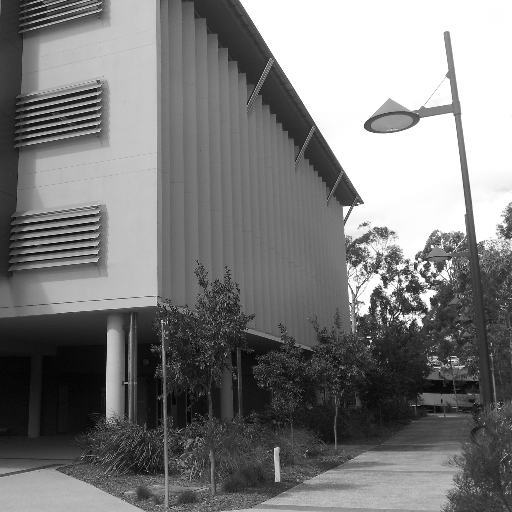
\includegraphics[width=4.2cm]{images/pc/original}
                \caption{original}
                \label{fig:PCSecOrig1}
        \end{subfigure}%
        \begin{subfigure}[b]{4.5cm}
                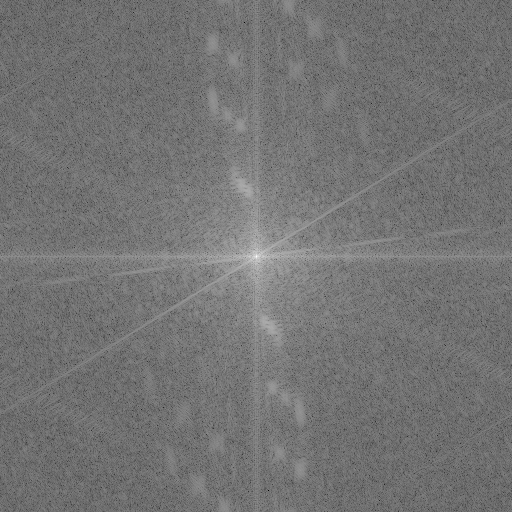
\includegraphics[width=4.2cm]{images/pc/magnitude}
                \caption{magnitude}
                \label{fig:PCSecMag}
        \end{subfigure}%
                \begin{subfigure}[b]{4.5cm}
                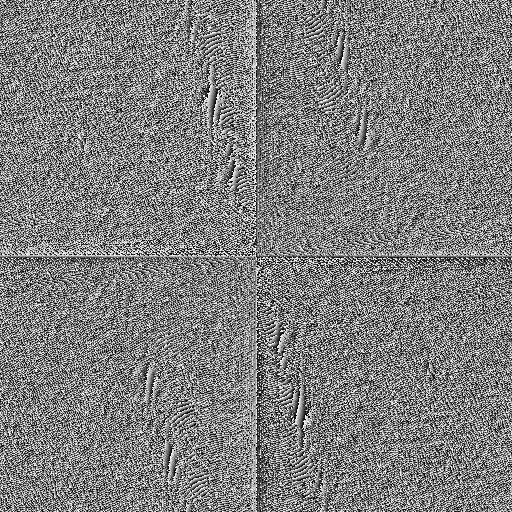
\includegraphics[width=4.2cm]{images/pc/phase}
                \caption{phase}
                \label{fig:PCSecPhase}
        \end{subfigure}%        
       \caption{The polar representation of the Discrete Fourier transform on an input image.}\label{fig:PCSecA}
\end{figure*}

Phase correlation is the process of using the frequency domain representation to perform image registration using correlation. In image processing, this allows us to find the translation parameters between two images (it does not work if rotation or scaling are introduced) efficiently. This can be performed by flipping one image before transforming both into the frequency domain. Since point-wise multiplication in the frequency domain causes convolution in the time domain, flipping one image causes correlation in the frequency domain which is what is required. Once this correlation is performed, the inverse Fourier transform is performed, the output image contains a peak which is used to compute the translation difference between the two images. This can be visualized in figure \ref{fig:PCSecCC}. Here, the original image is translated from figure \ref{fig:PCSecORY} to figure \ref{fig:PCSectrans} and the two are phase correlated producing the peak in figure \ref{fig:PCSecCCPC} which represents the translation between the two. \\


\begin{figure*}[t!] 
        \centering
        \begin{subfigure}[b]{4.5cm}
                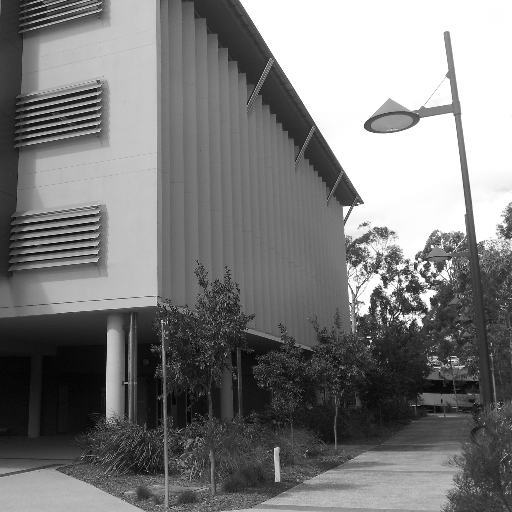
\includegraphics[width=4.2cm]{images/pc/original}
                \caption{original}
                \label{fig:PCSecORY}
        \end{subfigure}%
        \begin{subfigure}[b]{4.5cm}
                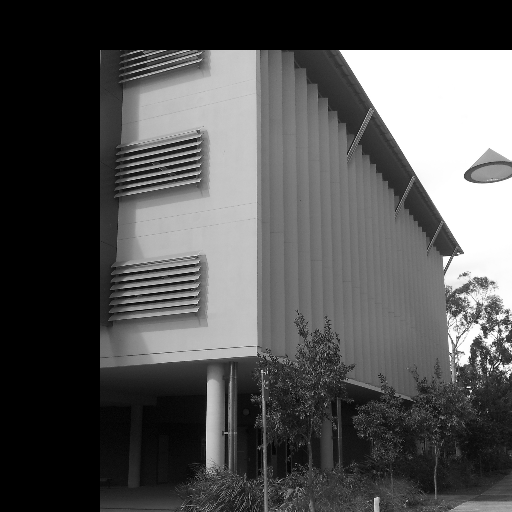
\includegraphics[width=4.2cm]{images/pc/translated}
                \caption{(a) translated}
                \label{fig:PCSectrans}
        \end{subfigure}%
                \begin{subfigure}[b]{4.5cm}
                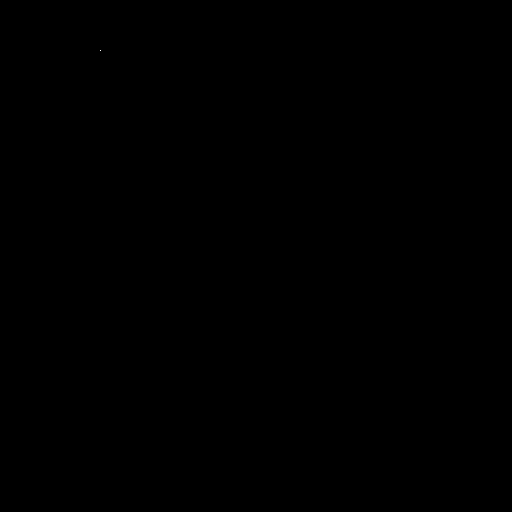
\includegraphics[width=4.2cm]{images/pc/phasecorrelation1}
                \caption{correlation}
                \label{fig:PCSecCCPC}
        \end{subfigure}%        
       \caption{Phase correlation used to align two images seperated by a translation.}\label{fig:PCSecCC}
\end{figure*}

The other parameters we wish to estimate for registration are the scale and rotation parameters, however another type of transform is introduced first. This image transform is called the log-polar transform. This transform re-arranges the pixels from euclidean 2D space $[x,y]$ to the polar space $[log(sqrt(x^2+y^2)),atan(y/x)]$ where rotation about the centre is turned into y-axis translation and scaling about the centre is turned into x-axis translation. This representation changes any rotation and scaling performed on the image into translation. Translation parameters can be easily found using phase correlation. This process can be visualized with the help of figure \ref{fig:PCSecB}. The problem is, the rotation and scaling has to be about the centre of the image, which is an issue if the images contain a translation effects. Luckily, in the magnitude of the polar representation of the frequency domain the effects of translation are not present. On top of this, any rotation or scaling (whether translation is present or not) occurs about the centre of the image. \\

\begin{figure*}[t!] 
        \centering
        \begin{subfigure}[b]{3.4cm}
                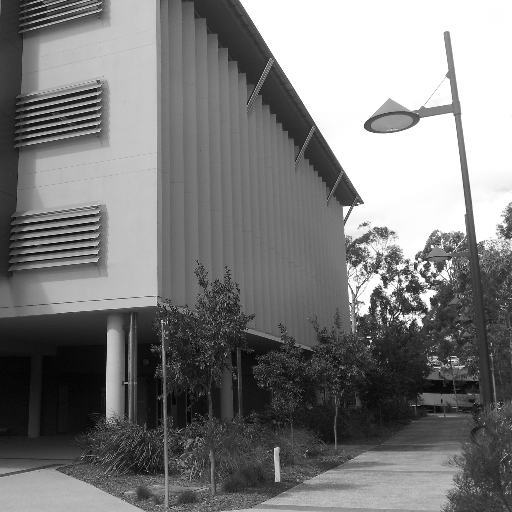
\includegraphics[width=3.2cm]{images/pc/original}
                \caption{original}
                \label{fig:PCSecOrig2}
        \end{subfigure}%
        \begin{subfigure}[b]{3.4cm}
                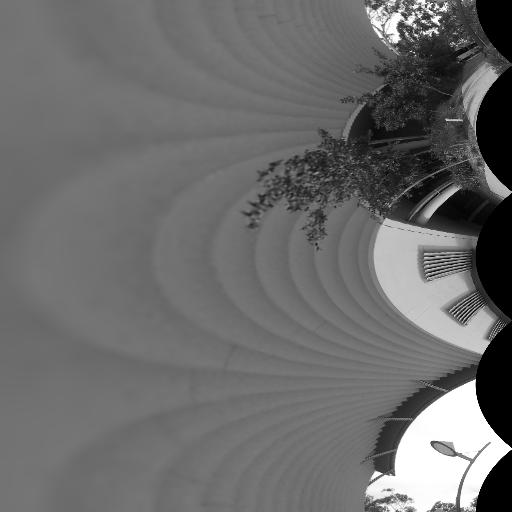
\includegraphics[width=3.2cm]{images/pc/logpolar}
                \caption{log-polar(a)}
                \label{fig:PCSecLP}
        \end{subfigure}%
         \begin{subfigure}[b]{3.4cm}
                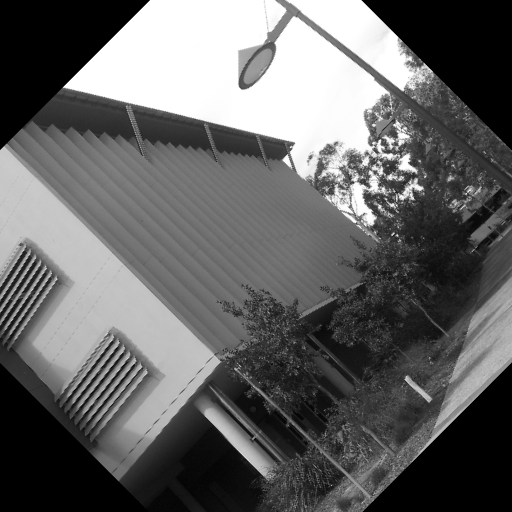
\includegraphics[width=3.2cm]{images/pc/rotation}
                \caption{rotated (-45${}^{\circ}$)}
                \label{fig:PCSecRot}
        \end{subfigure}%
        \begin{subfigure}[b]{3.4cm}
                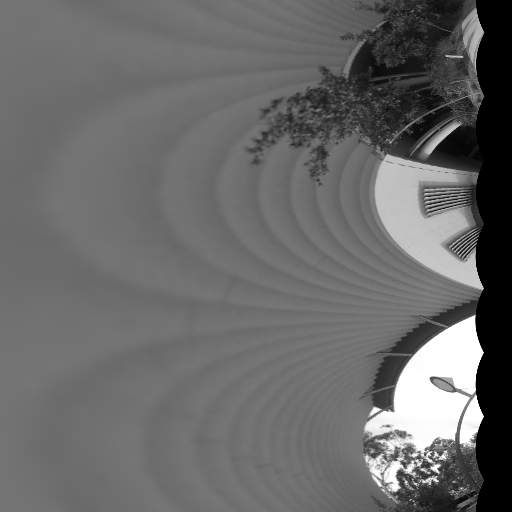
\includegraphics[width=3.2cm]{images/pc/logpolarRotation}
                \caption{log-polar(b)}
                \label{fig:PCSecLPR}
        \end{subfigure}
         \begin{subfigure}[b]{3.4cm}
                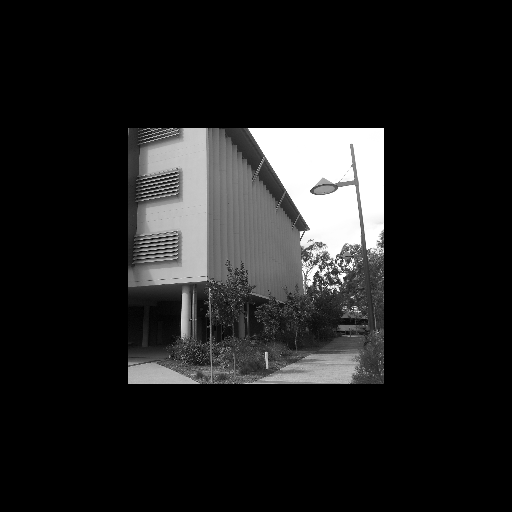
\includegraphics[width=3.2cm]{images/pc/scaled}
                \caption{scaled $\times$0.5}
                \label{fig:PCSecOrig2}
        \end{subfigure}%
        \begin{subfigure}[b]{3.4cm}
                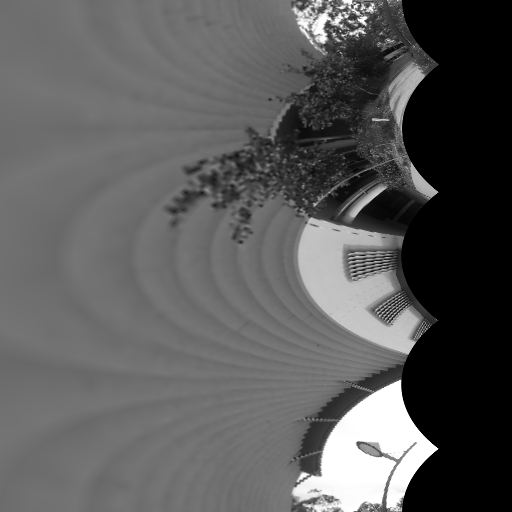
\includegraphics[width=3.2cm]{images/pc/logpolarScale}
                \caption{log-polar(c)}
                \label{fig:PCSecLP}
        \end{subfigure}%
                \begin{subfigure}[b]{3.4cm}
                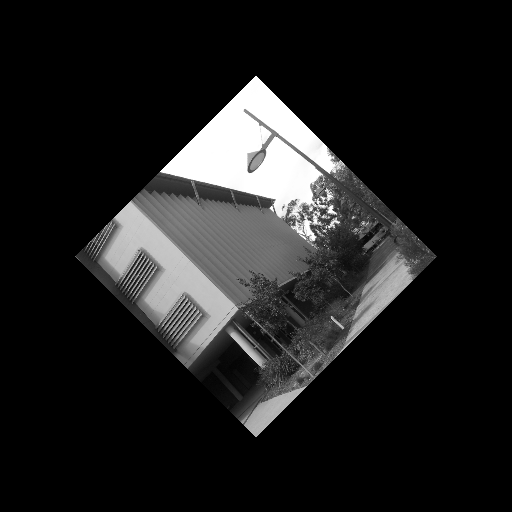
\includegraphics[width=3.2cm]{images/pc/rotationscale}
                \caption{rotated \& scaled}
                \label{fig:PCSecRot}
        \end{subfigure}%
        \begin{subfigure}[b]{3.4cm}
                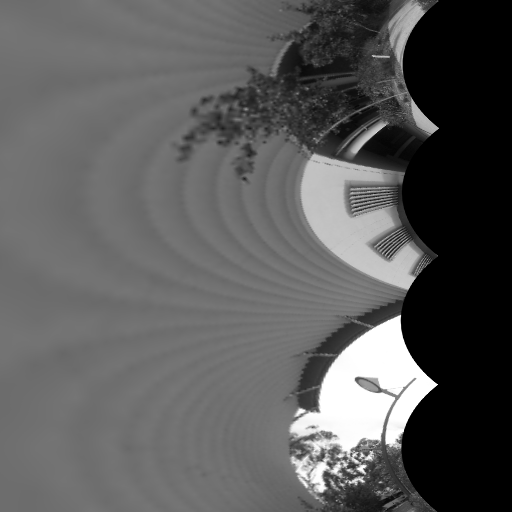
\includegraphics[width=3.2cm]{images/pc/logpolarRotationScale}
                \caption{log-polar(d)}
                \label{fig:PCSecLPR}
        \end{subfigure}%        
       \caption{The effects of the log polar transform.}\label{fig:PCSecB}
\end{figure*}

This allows the phase correlation method to recover the translation, scaling and rotational information between two images. First, the magnitude of the polar representation of both the images is computed. Then both magnitudes are log-polar transformed and phase correlated. This finds the scaling and rotational parameters. Both of the original images have their rotation and scaling reversed, then both images are phase correlated to undo the effects of translation, which is the final parameter to compute. In this way, translation, scaling and rotational parameters can be computed directly without the need for feature matching. \\

\section{Data Representations}

In this section, we describe several 3D data representations which are not only commonly used in 3D graphics and computer vision, but in 3D reconstruction as well. First, the popular mesh representation is described and a few popular methods for compression are surveyed. We also surveyed 3D volume and point cloud data as some other popular alternatives. Some newer representations are then discussed (image based methods and Signed Distance Functions). Finally, the octree, a common data structure used for 3D compression is discussed. \\

\subsubsection{Mesh}

Mesh data is popular due to its simplicity and integration into GPU technology. The 3D data is made of connected polygons which in turn are made of vertices. Edge information is typically defined implicitly. An example can be seen in figure \ref{MeshExamples}, vertices are represented using black dots, edges by lines, and polygons are labelled $F_0, F_1, F_2, F_3, F_4$. Here, vertex data define geometric information whilst edge and polygon data forms topological information. \\

For processing purposes, polygons are usually triangulated, which means all polygons are sub-divided into triangles. Any mesh may be triangulated, an example of this is provided on the right hand side in figure \ref{MeshExamples}. In a typical data representation, vertices are stored in a list and triangles are stored using three references to this list. The number of bits per vertex (bpv) is typically used to measure storage requirements for mesh data. \\

\begin{figure*}[t!] 
	\centering
	\begin{subfigure}[b]{6.8cm}
		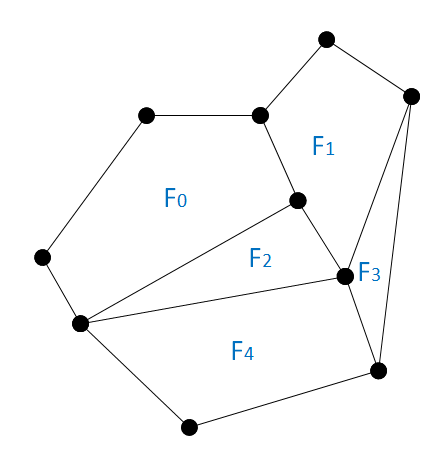
\includegraphics[width=6.5cm]{images/ch2/PolygonMeshExample}
		\caption{Polygonal Mesh}
		\label{fig:MeshExamples_polygon}
	\end{subfigure}%
	\begin{subfigure}[b]{6.8cm}
		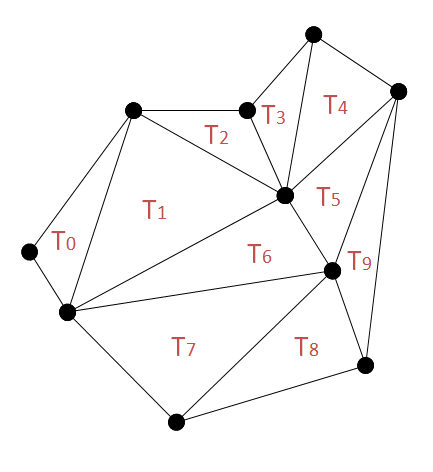
\includegraphics[width=6.5cm]{images/ch2/TriangleMeshExample}
		\caption{Triangulated Mesh}
		\label{fig:MeshExamples_triangle}
	\end{subfigure}%
	\caption{Mesh Types}
	\label{MeshExamples}
\end{figure*}


The Feature-Oriented Geometric Progressive Lossless Mesh coder (FOLProM) \cite{Peng10Feature} is a state-of-the-art codec which is progressive. It also aims to be an effective low-bitrate codec. It classifies segments of the mesh as being visually salient or not. Salient segments are preserved more during compression compared to non-salient ones. \\

Karni and Gotsman \cite{Karni00Spectral} proposed a lossy method which compresses a spectral representation of a mesh. This algorithm generally partitions the mesh and compresses each partition separately since it does not work on large meshes. Encoding a basis function for each partition, coefficients are quantized, truncated and entropy coded. Results show this method outperforms the previous state-of-the-art valence method \cite{touma98triangle} at coarse quantization levels. Bayazit et al. \cite{Bayazit103DMesh} also developed a progressive method based on spectral compression. This method is based on the region adaptive transform in the spectral domain and is advertised as a current state-of-the-art lossy 3D data compression method. \\

A lossy wavelet based compression system was proposed by Khodakovsky et al. \cite{Khodakovsky00Progressive}. This technique samples the mesh, and uses the wavelet transform to decorrelate the data. Coefficients are quantized and stored in a structure called a zero tree which increases compression performance. This method is also shown to outperform the valence method. Other wavelet approaches \cite{Guskov00Normal,Khodakovsky04Normalmesh} also sample the mesh and use a multi-resolution representation in which the data is described using local normal directions on the mesh surface. \\


\subsubsection{Point Cloud}

The point cloud structure stores a list of 3D points. This representation can be thought of as discrete samples of the surface of a real 3D object. Figure \ref{PointCloudExample} shows an example. This structure can be sampled using a variety of methods. These methods include both dense and sparse sampling, and sample steps can be either regular or irregular. Along with each vertex, a variety of attribute information can be stored. Point cloud data may be obtained via a 3D scanner or RGB-D camera. 

\begin{figure}[!htb]
\centering
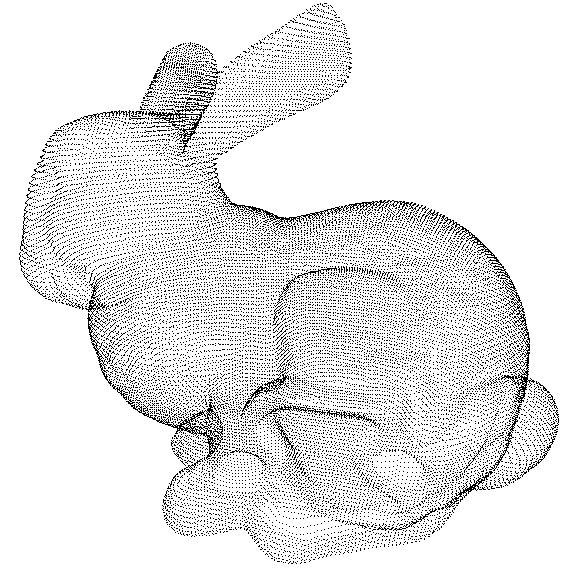
\includegraphics[width=6cm]{images/ch2/PointCloudExample}
\caption{A densely sampled point cloud of the Stanford Bunny.}
\label{PointCloudExample}
\end{figure}


\subsubsection{3D Volume}

In this representation, points are sampled into a 3D cubic space of sub-cubes called voxels. Such a space may have separate dimensions for width, height and depth or the space may be a true cube. In the context of 3D reconstruction, this data-representation is common and is used to store boolean values describing the occupancy of a space \cite{Rusinkiewicz02Real}. A visualization of a 3D volume showing a reconstruction is shown in figure \ref{fig:VolExamples}. This data type is useful because it allows for quick updates. Downsides include, large storage space and the fact that 3D space represented cannot be dynamically changed without significant cost. \\


\begin{figure*}[t!] 
	\centering
	\begin{subfigure}[b]{6.8cm}
		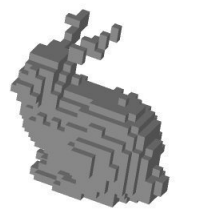
\includegraphics[width=6.5cm]{images/literature/bunnyVol32}
		\caption{Bunny sampled into a ${32}^3$ volume}
		\label{fig:Volume_Example32}
	\end{subfigure}%
	\begin{subfigure}[b]{6.8cm}
		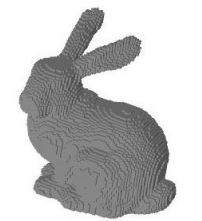
\includegraphics[width=6.5cm]{images/literature/bunnyVol128}
		\caption{Bunny sampled into a ${128}^3$ volume}
		\label{fig:Volume_Example128}
	\end{subfigure}%
	\caption{3D Volumes \cite{Passalis07General}}
	\label{fig:VolExamples}
\end{figure*}

\subsubsection{Signed Distance Functions}

A Signed Distance Function \cite{Curless96Volumetric} is a function which describes a 3D geometric space. Such a function takes a 3D location as $x,y,z$ coordinates as input and returns a single number value. The value describes the geometric detail of a particular object. Zero values are surface interfaces, positive values increase relative to the distance to the nearest surface and negative values represent the interior of the object. \\

SDFs may take the form of an equation or may be made discrete by means of discretization. In the context of 3D reconstruction we refer to the discrete SDF, an example of which is show in figure \ref{fig:SDFExample}. The SDF may be visualized by converting it to a mesh and rendering (by means of the marching cubes algorithm \cite{Cubes87High}) or by directly ray-casting the structure \cite{Parker98Interactive}. In the case of ray-casting, there is a significant advantage over the volumetric representation, that is the step size may be adjusted dynamically reducing render time. \\


\begin{figure}[!htb]
\centering
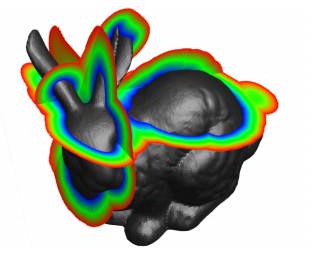
\includegraphics[width=6cm]{images/literature/SDFExample}
\caption{Distance Field Slices of the Stanford Bunny \cite{Sigg03Signed}.}
\label{fig:SDFExample}
\end{figure}

Canelhas \cite{Canelhas12Scene} did a masters thesis on an approach for camera tracking which makes use of an SDF. Similar to the work by Bylow et al. \cite{Bylow13Real} the project concentrates on object detection and recognition in an SDF although little evaluation was performed. Additionally storage was not considered. Kubacki \cite{Kubacki12Registration} proved the SDF is useful in estimating camera pose but only showed proof using synthetic data performing no comparative evaluation. Ren and Reid \cite{Ren12Unified}  demonstrated SDF based object tracking based on prior known models. \\

Elfes et al. \cite{Elfes87Sensor} use a Baysian probability of occupancy measure to decide if a point should be added to the grid and showed that SDFs may be used to fuse partial depth scans whilst impeding problems with mesh based reconstruction algorithms. The SDF representation was modified by Zach et al. \cite{Zach07Globally} to be more robust to noise. Bylow et al. noted that the SDF may be used to produce globally satisfied reconstructions in real time. \\


\subsubsection{Image Based Representations}

3D reconstructions may also be represented by means of elevation maps \cite{Herbert89Terrain} and multi-level surface maps \cite{Triebel06Multi} however these methods cannot store known and unknown areas of occupancy in a volumetric way. Additionally compression is often not considered and these methods do not have the search capabilities which the octree and volumetric representations have, nor the fine detail available in a mesh or point cloud representation. An example of an elevation map is shown in figure \ref{fig:HeightMapExample}.\\


\begin{figure}[!htb]
\centering
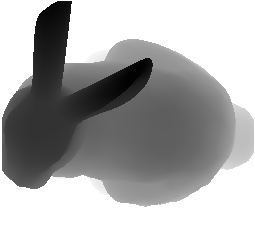
\includegraphics[width=6cm]{images/literature/HeightMap}
\caption{A Height Map of the Stanford Bunny.}
\label{fig:HeightMapExample}
\end{figure}

Gu et al. \cite{Gu02Geometry} devised a solution for representing 3D models as 2D images which are then compressed using state-of-the-art image compression methods (based on wavelets). To form this representation, the mesh is cut along a network of edge paths, opening the mesh into a topological disk, which is then sampled onto a 2D grid. Each pixel in the image has a corresponding coordinate in the model, with pixel neighbourhoods describing connectivity. Comparisons with the method by Khodakovsky et al. reveal the geometry image codec does not have as high compression performance. \\


\subsubsection{Octree}

The octree is a hierarchical data representation ideal for storage, search and processing of 3D data. Other hierarchical structures exist (such as K-D tree and BSP-tree) \cite{Samet06Foundations} but these are not as useful for compression as the octree, which is the aim of this research. The octree is described in detail below in section \ref{OTDesc}. An important technique based on the octree and used by many 3D reconstruction methods is the Octomap \cite{Wurm10Octomap}. It essentially records a volume occupancy grid using an octree. This method models data probabilistically whilst simultaneously reducing memory size. The Octomap representation is lossless and is can reduce the file size of the reconstruction by up to 50\%. \\

Other methods also explore the octree for 3D reconstruction and SLAM \cite{Fournier07Mapping,Meagher82Geometric,Fairfield07Real} however these methods do not really address storage advantages. 




\section{Depth Data Generation}
\label{DepthDataGenSection}

In 3D reconstruction, dense depth data is very important, without it there is no dense 3D reconstruction, only sparse mapping. This section introduces some techniques and research on different methods (both hardware and software) of depth data generation. In the first section the use of sensors which are capable of generating depth data is introduced. Next, methods using stereo camera pairs are discussed. Finally, monocular techniques are discussed. \\


\subsection{Sensors}

In 3D reconstruction, it is often ideal to use specialized sensors which capture reliable and dense depth data on a per pixel basis. One such camera is the RGB-D (Red, Green, Blue \& Depth) camera. These sensors are becoming more accurate and less expensive and are now found in mobile technologies. \\

Research by Zhang et al \cite{Zhang12Microsoft} used an RGB-D camera to generate smooth, continuously updating dense 3D reconstructions using only depth data. Here, using the data, 6 degrees of freedom were tracked. This techniques uses depth information only, and as such it works in the absence of visual light (it works in the dark) unlike passive camera approaches \cite{Klein07Parallel, Newcombe10Live,Stuhmer10Real} and techniques which use color data along with depth data \cite{Henry10Rgb}. \\

The Kinect is one such rgb-d camera. It uses a structured light based depth sensor along with an application specific integrated circuit to generate an 11-bit $640\times 480$ depth map at 30 times per second (real-time). \\

There is no doubt that these sensors are the easiest way to compute ready dense depth data for 3D reconstruction, but there are several drawbacks. Depth images contain holes. This is caused by a lack of structured light on a captured surface. Some materials simply do not reflect infra-red light (surfaces at steep angles or very thin objects). Also, when moving fast, the device easily experiences motion blur which leads to missing and incorrect data. \\

Some 3D reconstruction techniques use the approach of dense mapping and tracking via depth sensors and lasers. These approaches usually compute feature matches to align the frames or some sort of error minimization function.


\subsection{Stereo Cameras}

\label{StereoMethodsSection}

Stereo camera set-ups employ two cameras capturing a singular scene. Using a variety of techniques, depth data is computed from the stereo pair by measuring parallax. Stereo cameras may be calibrated or un-calibrated. Un-Calibrated stereo pairs require calibration using the Fundamental or Essential matrix, whilst pre-calibrated cameras require no further action before parallax may be computed. Using a variety of pose estimation techniques, the dense depth data may be integrated forming a 3D reconstruction. \\

In this section, some important techniques proposed within the area of depth data generation via stereo algorithms. Readers wanting to research techniques prior to 2005 are encourages to seed a survey by Scharstein and Szeliski \cite{Scharstein02Taxonomy}. \\


Sun et al \cite{Sun05Symmetric} presented an occlusion handling stereo matching algorithm. Their method incorporates a visibility constraint into the energy function for the belief propagation global optimisation method. Klaus et al \cite{Klaus06Segment} devised a stereo correspondence algorithm which uses colour segmentation combined with a self adapting matching score which minimizes the number of reliable occurrences. This method also uses belief propagation to assign a single disparity to each segmented region. Hirschmuller \cite{Hirschmuller05Accurate} proposed a semi-global matching method based on mutual information and approximation of a global smoothness constraint. \\

Yoon \cite{Yoon06Adaptive} presented work on a local method for computing disparity. In this method, the window is weighted based on geometric proximity and colour similarity. Darabiha et al \cite{Darabiha06Reconfigurable} presented an FPGA based local window stereo algorithm. This method obtains sub-pixel accuracy for 256$\times$360 images at 30 frames per second. Their window matching method uses correlation. Klaus et al. \cite{Klaus06Segment} devised a stereo method which segments the image before fitting regions with disparities. This fitting is based on interpolating depth values along each region. A self adapting matching score for segments is also used to maximize correspondences. Belief propagation is then used to optimize depth among the regions. \\


Yang et al \cite{Yang07Spatial} came up with a method which uses super pixel resolution to improve disparity images. First a depth map is computed at a lower resolution, it is then up-sampled to the same resolution as the corresponding colour image. The depth map is then used as a hypothesis to compute a cost volume, which is bilateral filtered. Then, a winner take all and a sub pixel estimation procedure are performed to estimate the full resolution depth map. This method is shown to improve sub-pixel resolution by up to 100 times compared to previous methods.\\


Sarkis et al \cite{Sarkis07Fast} improved the efficiency of the graph cut global optimisation based disparity algorithm whilst maintaining similar accuracy. Their method involves splitting the global space up using a quad-tree. Each space has an adapted energy function which is minimized using the graph cuts algorithm. Results show this method improves efficiency by up to 3 times over similar works. Wang and Zheng \cite{Wang08Region} came up with an inter-regional cooperative optimization based stereo correspondence technique. This method uses a local adaptive window based approach to compute an initial depth map. The original image is also segmented using a colour based mean shift technique. The segmented image and the initial depth map are then input into a region based optimization method.  \\


Yang et al. \cite{Yang08Near} attempted to solve the problem of stereo mapping for texture-less image regions. These regions are known to be difficult because there is less texture to correlate with. They use colour segmentation and plane-fitting with loopy belief propagation for error correction. Wang and Zheng \cite{Wang08Region} used a stereo method which uses image regions, plane fitting and segmentation as well as a novel region stereo optimization method. Ernst and Hirshmuller \cite{Ernst08Mutual} presented a GPU implementation of the semi-global matching technique (scan-line optimization) for stereo correspondence. Bleyer et al \cite{Bleyer09Stereo} devised a method which extracts disparities and alpha matting information at the same time. Alpha matting is used to generate artificial views for viewpoint effects. This method divides the image up into segments and computes the depth and alpha value for each of these segments. \\


Bleyer and Gelautz \cite{Bleyer09Temporally} presented a method for generating stereo disparity information from an un-calibrated stereo video. First, the video is segmented into scenes. Next, the two camera shots are calibrated before dynamic programming is used to optimize the disparity calculation. Then the disparity estimates are smoothed temporally in order to achieve robustness to disparity flickering. Hirschmuller and Sharstein \cite{Hirschmuller09Evaluation} presented a survey on stereo depth mapping with respect to radiometric differences. They investigated different metrics used in local matching methods as well as their relationship with radiometric variations. Also investigated were the effects of different filters: Laplacian of Gaussian (LOG), bilateral background subtraction, rank, SoftRank, census and ordinal. \\


In his masters thesis, Olofsson \cite{Olofsson10Modern} presented a survey and evaluation of various global and local stereo vision methods. He also presented a novel and efficient local method. This technique is shown to achieve state of the art results with some datasets. Bleyer et al \cite{Bleyer10Surface} introduced a method which models stereo images using smooth surfaces. This technique is based on the assumption that the entire scene is composed of a few smooth surfaces, and each pixel is a part of a surface. Colour segmentation is used to estimate different surfaces. Bleyer et al \cite{Bleyer11Patchmatch} presented a variation on the Patchmatch algorithm (PMA). PMA is a global optimisation method which models each pixel as a plane in 3D space. Each pixel is set to a random value within a larger region, as long as there is at least one close guess for the planes of one of the pixels, this information can be propagated. The default PMA performs spatial propagation, and uses adaptive support weighting to improve correspondence around the border. The method by Bleyer et al introduced view and temporal propagation to the original PMA. \\


Bleyer et al \cite{Bleyer11Object} later presented a joint stereo matching and segmentation algorithm. This method models segmented regions as objects having colour and a disparity distribution, they also use a novel 3D connectivity property for each object region. Lu et al \cite{Lu11Revisit} presented a method for increasing depth map quality given a colour original of the same scene at higher resolution. This allows disparity maps to be computed quickly by computing a lower resolution depth map before scaling-back the resolution. This method makes use of markov random fields and is unique in applying the technique to super pixel resolution in terms of depth mapping. This method is also uses state of the art disparity computation algorithms and so improves efficiency whilst retaining accuracy. \\ 


De-Maeztu et al \cite{De11Linear} presented a novel cost aggregation step for computing disparity images from a stereo pair. Their method works similarly to weighted pixel and scalable window routines but has complexity independent of window size. Unlike other cost aggregation methods, it can be used with colour and includes a novel disparity refinement pipeline. This method effectively filters the image so the pixels are weighted prior to performing some local disparity cost computation. Mei et al \cite{Mei11Building} presented a GPU based stereo correspondence algorithm which makes use of cost aggregation followed by scan-line optimization. Results show this GPU based algorithm is among the state of the art. \\


Mizukami et al \cite{Mizukami12Sub} described a novel method to reliably compute disparity cost volumes for sub-pixel depth mapping. It uses a combination of interpolation and an edge preserving filter. First a sub-pixel cost volume is computed, then this volume is filtered. Finally a two step sub-pixel disparity search is performed. Later, Zhu et al \cite{Zhu12Locally} presented a novel regularization method for stereo matching. This regularization method overcomes noise and captures general disparity at higher octaves and between regions. Lee et al \cite{Lee13Local} introduced a non-iterative one pass method for improving local stereo methods. To this end, a novel three mode cross census transform with a noise buffer is introduced. This method is used for both stereo image and video calculation. Stereo Video computation also makes use of optical flow. \\


Chen et al \cite{Chen13Novel} presented a local windowing based method which uses an adaptive support weight to achieve state of the art local method results. This method uses a novel trilateral filter as a weighting function. The trilateral filter extends the bilateral filter by adding in a component measuring boundary strength. Lu et al \cite{Lu13Patch} presented a super pixel variation of the Patchmatch stereo correspondence technique. Mei et al \cite{Mei13Segment} proposed a tree based approach for optimizing cost volumes. Their method first segments the image based on colour, instead of forming a graph between segments, and calculating the minimal spanning tree. A tree graph is created for each segment, then these graphs are linked with the optimization algorithm.\\


Tan et al \cite{Tan14Stereo} made an improvement to segmentation for use in disparity mapping. Since under-segmented regions contain disparity discontinuities (many methods assume regions have a global or planar based disparity value) and over-segmented regions contain noise, Tan et al proposed a new segmentation based stereo algorithm. This method makes use of a cost volume watershed algorithm and a new region merging strategy. It detects when regions are under-segmented and fixes the situation accordingly. Their method first computes information from an arbitrary segmentation method as well as an arbitrary local windowing disparity algorithm. This information is fed forward into their cost volume watershed. Using discontinuities in the cost volume, they further segment the regions, then a novel region merging method is performed, this final segmentation information is used for the global belief propagation disparity mapping method. \\


Yang \cite{Yang14Pattern} first developed a non-local disparity calculation algorithm based on using the minimal spanning tree to find an optimal solution using the cost volume. This method is supposedly improved upon by Vu et al \cite{Vu14Efficient}. This other method was designed for robustness to texture-less regions. It formulates the cost volume as a minimal spanning tree search problem. Yang et al also contributed some software for interactive depth of field effects called scribble2focus. Tan et al \cite{Tan14Soft} devised a multi-resolution based approach to disparity selection using cost aggregation over a cost volume. Results show this method performs close to global methods for reduced complexity. Lie et al \cite{Liu143d} posed the stereo correspondence problem in terms of interacting 3D entities. Their solution is aimed at curved feature depth estimation, and so they formulate their cost functions according to this constraint. \\



\subsection{Monocular Approaches}

Monocular depth generation includes any and all systems which use a single colour or grey-scale camera to generate dense depth data. Dense depth data is often computed using consecutive frames of a video sequence. If a relationship between frames is known, then the depth data may be either triangulated (given camera pose) or computed as in other stereo methods by calibrating image pairs first. The most popular technique is the computation of the essential matrix in order to perform stereo calibration. Once stereo calibration is performed, generic disparity computation methods (reviewed in \ref{StereoMethodsSection}. \\

An overview of computing the essential and fundamental matrix and the role they play in not only computing dense depth but computing camera pose is discussed in section \ref{FundamentalMatrixSection}. 



\begin{savequote}[8cm]
  ``He who controls the past controls the future.''
  \qauthor{George Orwell, 1984}
\end{savequote}
\makeatletter
\chapter{Reconstruction Techniques}

\section{Introduction}

In this section we review some of the crucial areas and techniques involved in both Simultaneous Localization and Mapping (SLAM) and registration. First, some important registration techniques are covered including both feature matching and phase correlation. Then, depth data generation is covered. These techniques assist with the generation of dense 3D data used for 3D reconstruction. Another important area: Pose estimation is also We begin with an overal tutorial on 3D-SLAM before covering registration. Next, 3D reconstruction data-representations and compression schemes are covered. 

%depth data generation and pose estimation

This section introduces several techniques used in SLAM and 3D Reconstruction for estimating pose. As mentioned, both of these research areas employ techniques to compute camera pose. Once camera pose is known, in the case of RGB-D methods, depth data may be integrated to generate dense 3D reconstructions. In the case of monocular or stereo approaches, dense depth information may be computed implicitly to varying degrees of accuracy. Once computed it may be integrated in a similar manner to RGB-D based methods. \\

There are many examples of camera pose being computed by robots \cite{Olson06Fast,Frese05Multilevel,Dellaert06Square,Thrun02Robotic,Nuchter056d,Grisetti07Efficient,Kaess08Isam}, in these cases, pose may be estimated by taking input from sensors (measuring wheel spins or thrust) \cite{Callieri04Roboscan}. It can also be computed via more complex methods based primarily on visual data \cite{Davison03Real,Klein07Parallel,Strasdat10Real,Jin00Real,Nister05Preemptive}. 
\\

If only monocular video data is available, the true scale of the map cannot be determined so true measurement based reconstructions are not possible \cite{Endres12Evaluation,Konolige08Outdoor, Paz08Large}. Furthermore many monocular algorithms only produce sparse reconstructions \cite{Davison03Real,Klein07Parallel}. \\

The first monocular slam system was presented by Davison in 2003 \cite{Davison03Real}. Davison's method uses a hand-held camera in real time to produce globally consistent sparse maps. It makes use of probabilistic filtering in its estimates of both camera pose (translation and rotation) as well as triangulation of sparse features. It was successful but is limited to in-door office environments because it requires large state vectors which grow with scene size. Another known limitation is that the use of sparse feature maps leads to poor accuracy. \\

Later, systems which split tracking and mapping (global optimization) came along such as the Parallel Tracking and Mapping Algorithm (PTAM) \cite{Klein07Parallel}. PTAM also performs camera tracking in real-time in small work spaces. It is essentially a bundle adjustment (a least squares solution to camera and feature optimization, see section \ref{sec:ba}) based pose estimation procedure. The tracking system runs in parallel at frame-rate speeds, performing robust n-point pose estimation with feature matching. In comparison to filter based methods, much more features can be packed into the map \cite{Strasdat10Real}. Approaches such as these typically accumulate drift (such as work by Beardsley et al. \cite{Beardsley97Sequential}) or perform off-line loop-closure optimization. \\

\subsection{The Fundamental Matrix and its Properties}

\label{FundamentalMatrixSection}

The Fundamental matrix method is especially useful in systems where monocular cameras are used for 3D reconstruction. From 2D point correspondences, the fundamental matrix may be computed. This leads to both the direct estimation of camera pose as well as stereo calibration parameters (which are required to compute dense depth information from monocular views). Here the Fundamental and Essential matrices, their estimation, properties and use in pose estimation are described.

To describe this technique, linear algebra is used. Note, all of the transforms required to represent imaging systems can be represented using $4 \times 4$ matrices and homogeneous $4 \times 1$ vectors. These important transforms include: 3D rotation, scaling, shearing/skewing, mirroring, translation and perspective transforms. Rather than describing camera capture using projecting rays, linear algebra provides further capabilities and clearly defines the estimation process of the fundamental matrix. 

In figure \ref{fig:INTRO_FMA1} there are two camera systems. We begin with an explanation as to how point $Q$ is projected from 3D onto the 2D point $Q_{1}$ is discussed. First, $C_{1}$ is defined as the origin (later this allows rotation and perspective transforms to more easily be performed). In order to do this, $C_{1}$ can be subtracted from itself (to become the origin) and so it is also subtracted from $Q$ as well. To this end, a $4 \times 4$ translation matrix, $T$ is used. Next, rotation is performed in order to align the camera's axes with the x, y and z axes. The camera's axes can be defined using three vectors. One pointing directly ahead where the camera is facing (piercing the centre of the projection frame), another pointing directly to the right perpendicularly (orthogonal to the first), the final points above the camera, aligned orthogonally with the previous two vectors. \\

These three axes can be placed into the columns of a $4 \times 4$ homogeneous matrix. This forms a matrix which rotates an aligned camera's axis to face the direction where $C_1$ currently points to. In other words, it performs the exact opposite of what is needed. Since this matrix is orthogonal (known because the column vectors are all perpendicular) the inverse transform is simply the transpose of this matrix. This rotation matrix is defined as $R$. Next, there may be a lateral alignment, this is a translation which further aligns the points to the centre of the frame. This is performed using another $4 \times 4$ matrix, $L$. Finally, another $4 \times 4$ matrix, P is used to project the point $Q$ to the 2D point, $Q_1$. The entire projection can be performed by multiplying these matrices together, $Projection = P * L * R * T$. Here, $P * L$ are known as the intrinsic parameters whilst $R * T$ are called the extrinsic parameters. Due to the imperfect nature of the camera lens, the intrinsic camera matrix often has distortion, this becomes important later when we define the difference between the fundamental matrix and another matrix introduced, the essential matrix.

\begin{figure*}[!htb]
	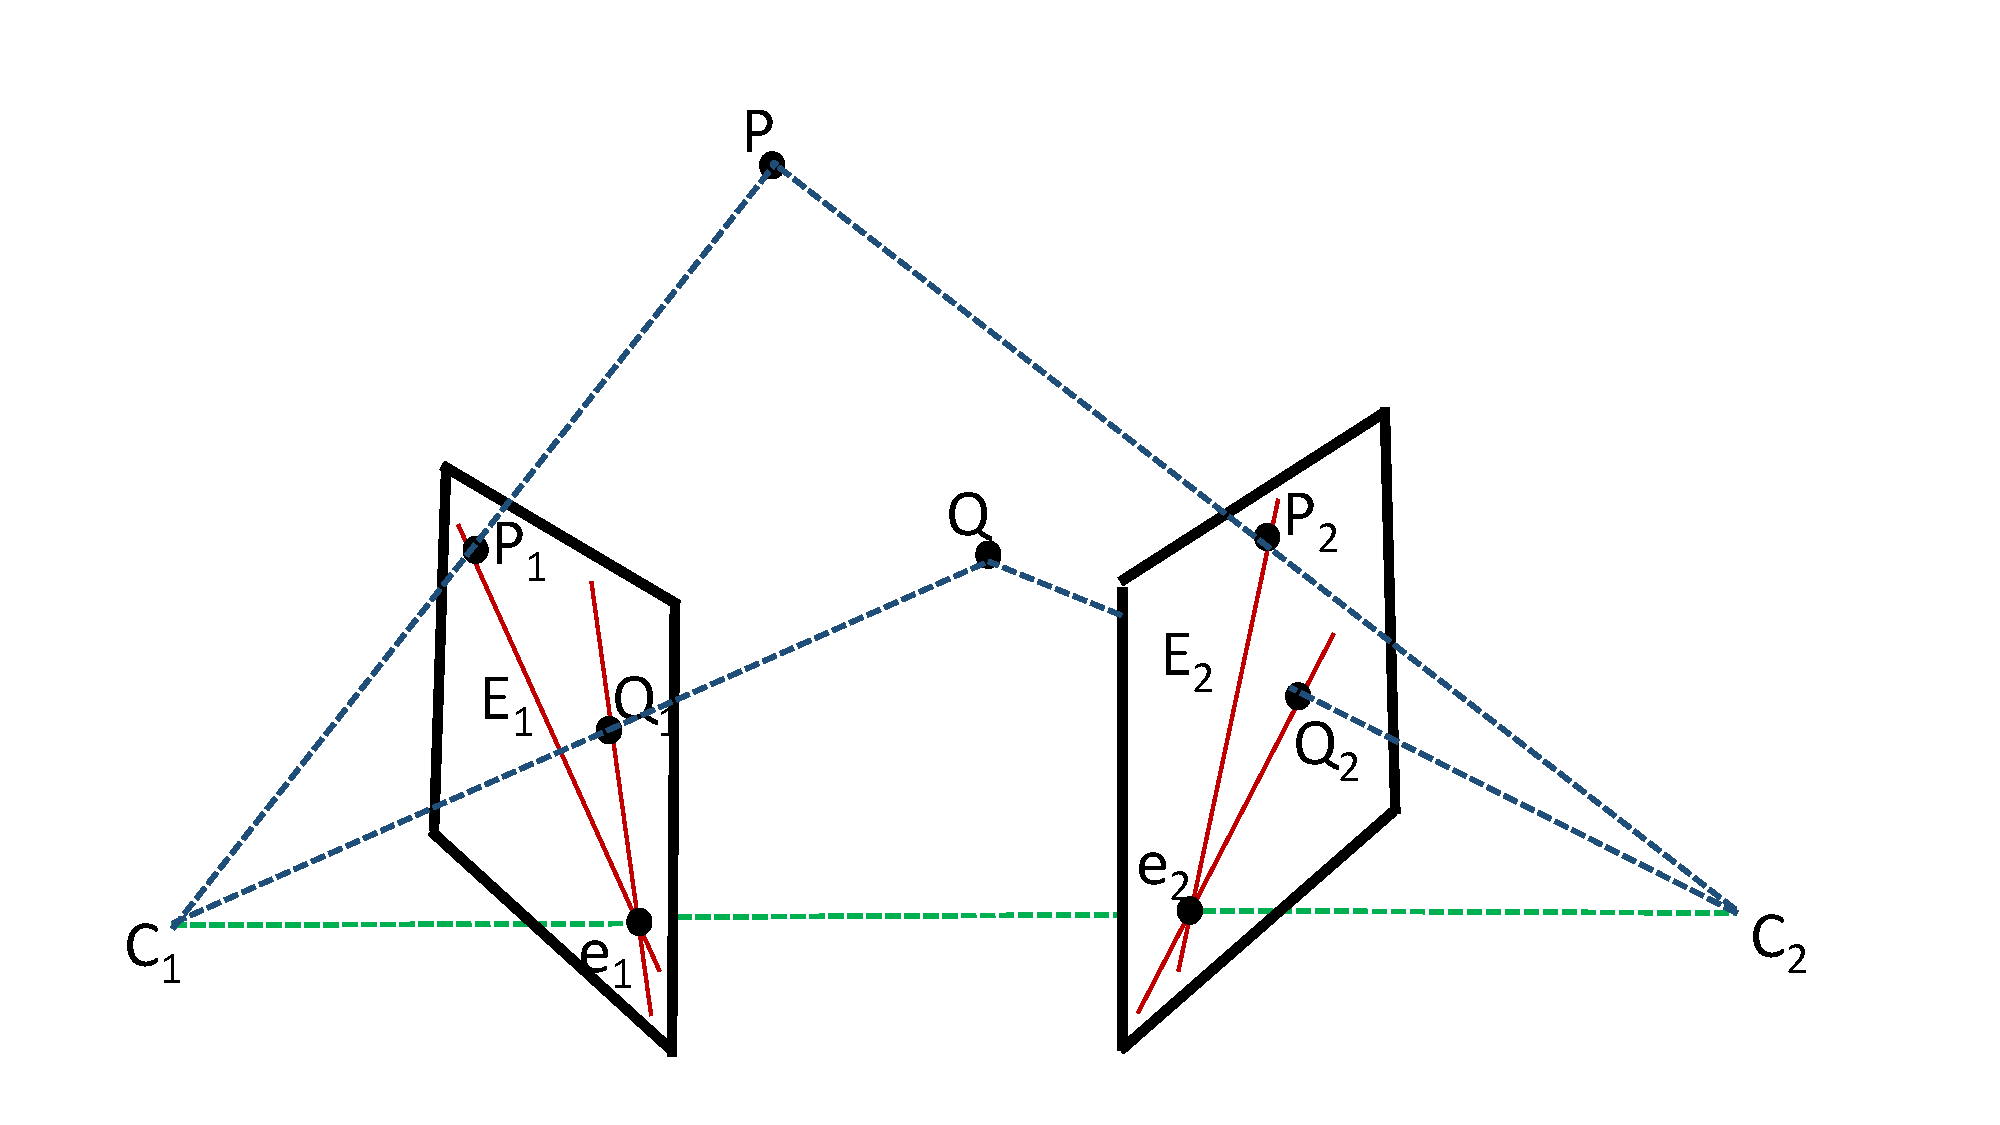
\includegraphics[width=5.0in]{images/introfm1}
	\caption{A pair of cameras viewing two points. This figure is a reconstruction of the figure on page 492 in Computer and machine vision: theory, algorithms, practicalities \cite{Davies12Computer}.}
	\label{fig:INTRO_FMA1}
\end{figure*}  

Using the steps described and looking at figure \ref{fig:INTRO_FMA1}, it has been identified how 3D point $P$ is mapped to both of the frames with cameras $C_1$ and $C_2$. Projecting point $P$ onto the two frames gives points $P_1$ and $P_2$ respectively. $V_1$ is defined as a vector relating $P_1$ and $P_2$. It is formed by normalising the vector from $C_1$ to $P$ $(P - C_1)$, and $V_2$ is found similarly $(P - C_2)$. The relation between these vectors is the essential matrix \cite{Davies12Computer}, $E$. The specific relation is $V_2^{T} * E * V_1 = 0$. The depth of $P$ is unknown and cannot be estimated directly unless an investigation is performed on the particular camera system in use. The precise perspective transform and associated distortion must be known. Fortunately, both the depth and the perspective are cancelled in this matrix formulation, and so we can specify the relation using only the 2D points, $P_1^T * E * P_2 = 0$. \\

This formula is based on the assumption that no distortion is present in the camera system. In this case, both of the cameras may have distortion. We represent this distortion here using matrices $G_1$ and $G_2$. If both shots are taken with the same camera, it is assumed that $G_1$ is equal to $G_2$. We therefore relate the theoretically precise $P_1$ and $P_2$ with their real-world equivalents (which have distortion) $D_1$ and $D_2$ by $P_1 = Q_1^{-1} * D_1$ and $P_2 = Q_2^{-1} * D_2$. Inserting this into the essential matrix formulation we have, $(Q_1^{-1} * D_1)^T * E * Q_2^{-1} * D_2 = D_{1}^{T} * {Q_1^{-1}}^{T} * E * Q_2^{-1} * D_2 = 0$. The presence of this distortion is the difference between the essential and fundamental matrices with the fundamental matrix being $F = {Q_1^{-1}}^{T} * E * Q_2^{-1}$. If no distortion is present, the fundamental matrix is equivalent to the essential matrix. \\

Using the Essential or Fundamental matrices, we may compute both camera pose, and stereo calibration. The camera pose is computed by using singular value decomposition (SVD) on the essential matrix. This breaks it down into 3 matrices ($W$, $U$ and $V$). Then, both the translation part (equation \ref{eqn:FundaTrans}) and rotational part (equation \ref{eqn:FundaRote}) of the camera pose may be computed.

\begin{equation} \label{eqn:FundaTrans}
Translation Matrix = W\left[
\begin{array}{ccc}
0 & 1 & 0 \\
-1 & 0 & 0 \\
0 & 0 & 0 \\
\end{array}
\right]W^{T}
\end{equation}
\myequations{Translational Part of Fundamental Matrix}

\begin{equation} \label{eqn:FundaRote}
Rotation Matrix = W\left[
\begin{array}{ccc}
0 & -1 & 0 \\
1 & 0 & 0 \\
0 & 0 & 0 \\
\end{array}
\right]V^{T}
\end{equation}
\myequations{Rotational Part of Fundamental Matrix}

Looking at figure \ref{fig:INTRO_FMA1} again, line $E_1$ represents an epipolar line, this line lies on the plane in which both cameras and point $P$ lie on. Line $E_1$ is the epipolar line belonging to the left frame and $E_2$ is the epipolar line belonging to the right frame. Point $e_1$ is the epipole of the left frame and point $e_2$ is the epipole of the right frame. Epipoles are the projection of one camera's location onto the frame of another camera. The projection of $C_2$ onto the left frame by camera $C_1$ is the epipole $e_1$. If the fundamental matrix is multiplied by a particular point it produces a vector in $R^3$ which represents the epipolar line as $[a b c]^T$ in which $a,b$ and $c$ represent the line equation $ax^2 + bx + c$. The epipolar line corresponding to $Q$ and $Q_1$ passes through a common point with the other epipolar line $E_1$. All epipolar lines intersect at the epipole. \\

The fundamental matrix may be computed using point matches between images. As mentioned the fundamental matrix can be used to perform image rectification and estimate camera pose. As shown, the fundamental matrix, epipolar lines and epipoles can be estimated from point correspondences. If the epipoles are known, then the direction in which the other camera resides is also known. \\

The basic pipeline for the fundamental matrix method begins with feature matching. Using matches, the fundamental matrix is typically estimated using an outlier filtering strategy such as Random Sample Consensus (RANSAC). Then extrinsic camera information is estimated and images are rectified so that disparity information can be computed. This may be used to compute dense depth data required for 3D reconstruction. One downside to this method is that the scale of the translation computed is not true. \\


Monocular Feature based SLAM systems use feature matches to estimate camera pose and location changes across frames \cite{Davison02Simultaneous}. Variations of this method use different features including: corners and lines \cite{Jeong06Visual}, image patches \cite{Silveira08Efficient} and exemplar feature matching \cite{Chekhlov07Robust}. SIFT features are used most often in SLAM \cite{Jensfelt06Framework,Pollefeys08Detailed,Beall11Bundle,Eudes10Fast}, in addition FAST features have been explored \cite{Kundu10Realtime,Leelasawassuk133d,Konolige10View,Konolige08Frameslam}. Beall et al. \cite{Beall11Bundle} made use of both SIFT and SURF features in their underwater SLAM system. Real-time monocular SLAM systems based on this approach have also been proposed \cite{Chekhlov07Robust,Pollefeys08Detailed}. RANSAC is often used in monocular SLAM \cite{Eudes10Fast,Kundu10Realtime,Konolige10View,Konolige08Frameslam,Pradeep13Monofusion} to remove outliers. Without RANSAC, incorrect camera parameter estimates would prevent any accurate pose estimation in all but synthetic data. Bundle adjustment is also used as an additional step to refine camera parameter estimation \cite{Eudes10Fast} (section \ref{sec:ba}).  \\


\subsection{Feature Matching and RANSAC}
\label{FMANDFM}

Feature matching together with RANSAC may be used to compute the Fundamental and Essential matrices which leads to camera pose estimates. The process of estimating the Fundamental matrix is simple, but in practice noise often makes accurate estimation difficult. Furthermore, the intrinsic camera parameters must be known prior in order to apply such a technique, else noise decimates the ability to accurately estimate camera pose and calibrate frames for stereo correspondence. \\

Another, more common way to use feature matching with RANSAC \cite{Fischler81Random,Chen99Ransac} is to compute the camera pose directly using multi-frame RGB-D data. Alternatively (as mentioned in section \ref{DepthDataGenSection}), dense depth information may be recovered using monocular and stereo camera set-ups as well. \\

This method first computes feature matches between two given frames. These matches along with the 3D location of each corresponding match (projected using the dense depth data) are used as input to RANSAC.\\

RANSAC is an iterative algorithm which works by repeatedly selecting a subset of input data, computing a model on the subset and testing that model on the global superset. During this repeated process, the subset with the best classification (lowest error or greatest strength model) is chosen for the final model. RANSAC is useful because it is an effective and capable algorithm for filtering out outliers. \\

In the case of camera pose estimation, the subset is used to compute the camera pose (using singular value decomposition) and the camera pose which minimizes the global error is chosen as the best camera pose. Here we describe how to compute the camera pose given a set of 3D points matched from one frame to another. Given two identical length arrays of 3D points, $P$ and $Q$, for each point in $P$, $P_i$ matches best with point $Q_i$. The covariance matrix $X$ is then computed based on $P$, $Q$ and their mean values. The calculation for $X$ is shown in figure \ref{eqn:CovarMatForFMRansac}.


\begin{equation} \label{eqn:CovarMatForFMRansac}
X = \sum_{i=1}^{N} (P_i - P_{mean}) \times (Q_i - Q_{mean})^T
\end{equation}
\myequations{Covariance Matrix for Computing the Fundamental Matrix}

Given the covariance matrix $X$ we compute its singular value decomposition matrices $W$, $U$ and $V$. Then the rotation part of the pose may be computed as $R = V^T \times U^T$. The camera movement can be computed by $T = -R \times P_{mean} + Q_{mean}$. If scale must be computed, it can be computed as $S = (Q_i - Q_{mean}) / (R \times(P_i - P_{mean}))$ for any $i$. \\

Computing 3D reconstructions using feature matching is often preferred as close competitor ICP is often unnecessary and expensive \cite{Endres12Evaluation}. However, the computation of pose without ICP with feature matching only is still non-trivial because of the following issues:


\begin{itemize}
\item Synchronization problems between the RGB camera and infra-red camera shutters cause inaccurate pose estimates. 
\item Feature matches often occur at depth jumps (the interpolation of computed depth at object boundaries). This also leads to inaccurate pose estimates.
\end{itemize}


\subsubsection{RGB-D SLAM}

Endres et al. \cite{Endres12Evaluation} presented a dense 3D reconstruction technique using RGB-D data from the Kinect sensor based on feature matching and RANSAC. They also evaluated their technique under different illumination and camera movement speed conditions. It is able to operate at near real time speeds in small in-door environments. This method begins by feature matching RGB images across frames. Using the projected 3D points available for each pixel in the depth map, RANSAC \cite{Fischler81Random,Huttenlocher91Fast} is used to compute the camera pose across frames. These poses are optimized globally using the $g^2$o graph optimizer (see section \ref{Sec:G20}), the Octomap representation \cite{Wurm10Octomap} is used to voxelize the 3D points before storing them in a volumetric occupancy map. Since this system is based on feature matching, Endres et al. evaluated three different feature matching techniques: SIFT \cite{Lowe04Distinctive} , SURF \cite{Bay06Surf,Bay08Speeded} and ORB \cite{Rublee11Orb}. ORB feature matching is used because it is faster than SIFT and SURF with slightly less accuracy, the authors also evaluate a GPU implementation of SIFT \cite{Wu07Siftgpu}. Endres et al. evaluate their algorithm using their own benchmark \cite{Sturm11Towards}. Results show it can handle up to 50 degrees of rotation per second, and speeds of up to 43 centimetres per second.  \\


This system is divided into a front-end and a back-end. The front-end performs feature detection, matching and sensor pose estimation via the RANSAC method whereas the back-end performs non-linear pose optimization using the $g^2o$ optimization procedure and integrates these results into an occupancy grid based on the Octomap. A diagram of the combined front-end and back-end systems is given in figure \ref{Endres12EvaluationPipeline}. 


\begin{figure}[!htb]
\centering
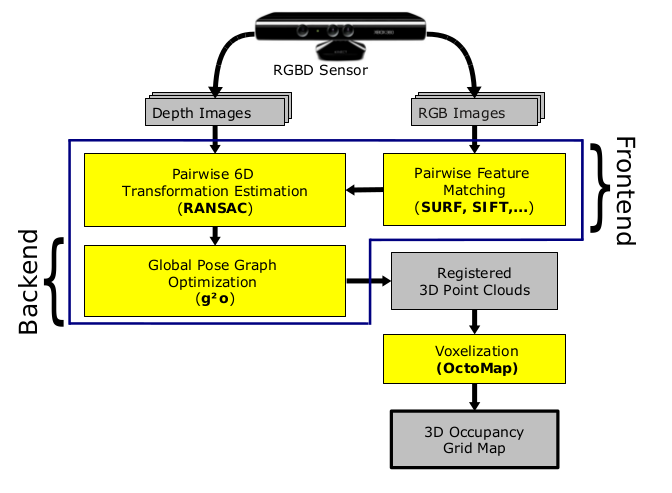
\includegraphics[width=12cm]{images/ch1/Endres12EvaluationPipeline}
\caption{RGB-D SLAM Pipeline used by Endres et al. \cite{Endres12Evaluation}}
\label{Endres12EvaluationPipeline}
\end{figure}


The front-end uses OpenCV \cite{Bradski08Learning} for feature matching. During the feature detection process, the Hessian threshold is used to keep the total number of features constant. This is required because pose may not be able to be computed if there aren't enough features, on the other hand, too many features typically leads to many false positives in the feature matching schema. This results in sub-par performance due to a likely lengthier RANSAC process. \\

As mentioned, these matched features (and thus matched 3D points) are used with RANSAC to compute pose \cite{Umeyama91Least}. During the RANSAC process, corresponding points with distances below 3cm are considered inliers. The inliers are then used exclusively to compute a finer pose. This method of pose estimation is fast but the computational complexity depends on the number of features computed. For each frame, the pose relationship with 20 previous frames (including the most recent 3) is computed in parallel on the GPU. Then the final computed pose is given to the back-end. If an accurate pose cannot be computed, constant motion is assumed. \\

\subsubsection{Fast Odometry from Vision: FOVIS}

Another technique which is based on feature matching is the FOVIS (Fast Odometry from Vision) technique \cite{Huang17Visual}. FOVIS works in 6 stages. In the first two stages, the RGB-D image data is collected and put through a low-pass filter, Gaussian scale space is computed and then FAST features \cite{Rosten06Machine,Rosten05Fusing} are computed. In the next stage, initial camera rotation estimation is computed by minimizing the sum of squared errors between down sampled versions of consecutive image frames. In the fourth stage, feature matching is performed, using the SAD (sum of absolute differences) metric and sub-pixel resolution. In the fifth stage, outliers are removed using a feature match graph and a greedy algorithm to find maximal cliques \cite{Hirschmuller02Fast,Howard08Real}. \\

In the final stage, the full camera pose is estimated using Horns method \cite{Horn87Closed}. This technique minimizes an error function in computing the camera pose. The FOVIS method then optimizes this by minimizing the re-projection error using a non-linear least squares method. \\

Whelan et al. \cite{Whelan12Kintinuous} extended Kinectfusion allowing it to map larger areas. They compared ICP with FOVIS and found that FOVIS contributed less drift but lacklustre models compared with ICP. Whelan et al. also proposed a technique for incrementally creating a triangle mesh as the reconstruction was built. This method uses multi-threading, and uses pose graphs for further optimization (see section \ref{Sec:G20}).

\subsection{ICP}

\label{ICPSection}

Iterative Closest Point (ICP) \cite{Besl92Method,Rusinkiewicz01Efficient,Segal09Generalized} is an iterative optimization method used to register 3D data. It works by iteratively minimizing registration error given two sets of point clouds and is a popular method for estimating 6-DOF (6 degrees of freedom) camera pose. The algorithm works by computing the closest point using some metric (usually Euclidean distance) for each of the points in the first point cloud. Then computing a transform which minimizes either the Euclidean distance error or some other error metric \cite{Steinbrucker11Real,Tykkala11Direct,Kerl13Robust,Chen92Object,Stuckler12Robust}. \\

The points are then transformed by the computed transform and this process is repeated which is supposed to iteratively minimize registration error. The 6-dof (3 axes of rotation plus 3 axes of translation) are commonly computed using the method described in section \ref{FMANDFM}. Various distance metrics have been researched including the point-plane metric \cite{Chen92Object}. This metric improves convergence rates and is used for surface reconstructions which contain additional information about the normals of each points. This algorithm is highly successful in generating accurate 3D reconstructions but it does have a few issues. \\

The first issue is that whilst computing the best transform using ``feature matches'' (which are nearest points between consecutive frames) is a simple concept, computing these closest points for each input point is expensive. This can be improved using the projective data association algorithm \cite{Blais95Registering} usually used by exploiting a projected version of the 3D data. The efficiency issue can also be improved using a coarse-to-fine scheme. \\

Another issue is that ICP is limited to small rotation, translation and scale. If larger transforms are present (especially scale in the case of general registration) ICP will usually get stuck in a local minimum and fail to register \cite{Mitra04Registration}. The final issue is that of slippage \cite{Whelan13Robust}. ICP tends to fail in environments with little texture. Here we present some important algorithms which use ICP in 3D reconstruction.

\subsubsection{Feature Matching, RANSAC and ICP Refinement}

Some systems make use of feature matching with RANSAC (see section \ref{FMANDFM}) for pose estimation and ICP for further alignment \cite{Engelhard11Real, Henry10Rgb}. These methods are very similar and make use of the advantages of both the faster and more robust feature matching method and the more accurate ICP optimization inclined method. \\

Henry et al. \cite{Henry10Rgb} presented work on a 3D mapping method which combines Feature Matching and RANSAC (similar to \cite{Endres12Evaluation}) with ICP. This method makes us of an RGB-D camera for sparse feature matching. Feature matching is used with RANSAC and the technique described in section \ref{FMANDFM}. ICP is used for refinement of the initial prediction. If loop-closure is required, a constraint is added to the 3D pose graph \cite{Kummerle11G} and is used to close the loop. A Surfel \cite{Pfister00Surfels} volumetric fusion method is used to represent and store the 3D reconstruction. This technique may be used for robot localization and path planning \cite{Hornung10Humanoid}. Endres et al. \cite{Endres12Evaluation} compared this method with theirs using a standard benchmark \cite{Sturm12Benchmark}.  \\

\subsubsection{Non-Rigid Alignment}

In addition to rigid alignment ICP is used by Pauly et al. \cite{Pauly05Example,Brown07Global} to align depth maps using non-rigid transforms. In the method by Brown and Rusinkiewicz \cite{Brown07Global}, ICP is used to first align the point clouds using a rigid alignment, then global feature positions are found using a relaxation method. Finally, 3D point sets are warped to final positions using thin plate splines. Brown and Rusinkiewicz state that this outperforms rigid based alignments.


\subsubsection{Kinect Fusion}

Newcombe et al. \cite{Newcombe11Kinectfusion,Izadi11Kinectfusion} proposed an accurate, real-time dense 3D reconstruction algorithm which works well on complex indoor environments. This algorithm computes relationships between depth map frames generated using the Microsoft Kinect \cite{Zhang12Microsoft} sensor. By aligning depth maps this method is capable of tracking both camera pose and location as well as generating dense 3D reconstructions. Only depth data is used in alignment computations and because the Kinect is a structured-light based depth sensor, Kinect Fusion works under any lighting condition, including complete darkness. Since this method uses the Kinect and GPU (both considered a commodity) the technique may be considered inexpensive. \\

The method works by computing camera pose, transforming depth data by computing pose (frame-by-frame) and fusing this data into a global surface volume. It uses a coarse-to-fine grain ICP algorithm to compute camera pose. During the ICP phase, the target points come from the entire globally matched previous frames. Therefore, this method is considered global rather than frame-to-frame based. Such a method has direct advantages over frame-by-frame feature matching, since all data is used to compute pose. The downside, is that this method fails to find global solutions due to the nature of ICP. This may occur when some frames must be skipped due to motion blur, or the camera passes over surfaces which do not reflect infra-red light. \\

\begin{figure}[!htb]
\centering
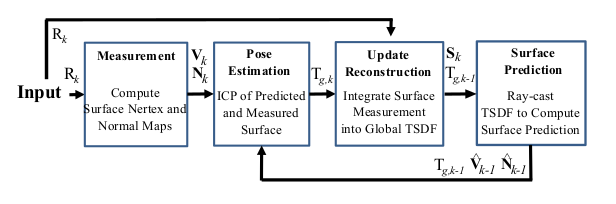
\includegraphics[width=12cm]{images/ch1/Newcombe11KinectFusion1}
\caption{Kinect Fusion Algorithm Pipeline \cite{Newcombe11Kinectfusion}}
\label{KFusionPipeliciteHne}
\end{figure}

Kinect Fusion has four main steps as illustrated in figure \ref{KFusionPipeliciteHne}. The first step performs pre-processing on the depth data and generates additional information for later use. Each depth map frame is first passed through a bilateral filter. From this, a dense vertex map (map of 3D points projected using a known projection matrix associated with the Kinect) is generated, as well as a normal map. For both the vertex and normal maps, a 3-level image pyramid is constructed. This makes the coarse-to-fine grain ICP technique possible. \\

Next, the dense coarse-to-fine grain ICP is used to compute pose between the fused frames and the current frame. The authors exploit the fact that the transformation between frames is small because camera motion is slow when computing against every frame. With coarse-to-fine grain ICP they use projective data association \cite{Blais95Registering} and the point-plane metric for pose optimization \cite{Rusinkiewicz02Real}. The ICP based pose estimation computes pose given both a predicted and measured depth map. \\

After estimating camera pose relating to the globally fused model, each frame must be integrated into that model. The Kinect Fusion algorithm uses a truncated SDF (TSDF) representation. This is a SDF volume where the distances for each voxel are capped by some value. The TSDF uses a volume resolution of $512\times 512\times 512$. They use the TSDF, rather than relying on a linear but accurate discrete SDF transform \cite{Rasch09Remarks} because of the computation required in calculating the discrete SDF for volumetric data. \\

As mentioned, Kinect fusion uses pose prediction and fuses each depth map into the TSDF representation. In this way, they align and fuse each depth map to the global 3D reconstruction. Therefore, global loop closure is not required. This may have a negative side effect as some frames which have larger resolutions may be heavily quantized in order to be fused with the SDF, especially thin surfaces. These features may also negatively impact ICP in estimating pose. \\


\subsubsection{FOVIS and ICP Integration}

Whelan et al. improved \cite{Whelan13Robust} upon their previous method \cite{Whelan12Kintinuous} by integrating FOVIS and ICP together on the GPU, and added an advanced colour fusion model to the technique. The primary improvement lies in switching between FOVIS and ICP. Whenever the error using FOVIS is too high, ICP is used. They also integrate using a global model rather than a local one. \\


\subsection{Direct Optimization Methods}

\subsubsection{Optimization over a Signed Distance Function}
\label{BylowsSection}
In 2013, Bylow et al. \cite{Bylow13Real} presented a novel method which reconstructs static indoor environments in real time using RGB-D data captured using the Asus Xtion Pro Live sensor. Their system is able to generate accurate 3D RGB coloured models of the environment in real-time by optimizing for 6-DOF in terms of accurate projection of new depth map frames into an existing global SDF model. Their method uses Gauss Newton optimization over a SDF representation on a laptop with an NVIDIA GPU. Unlike Kinect Fusion \cite{Newcombe11Kinectfusion}, this method optimizes directly in the SDF. Camera pose is computed by finding a rotation and translation which minimizes the error in projecting depth images into the SDF. Compared to Kinect Fusion, this technique is more robust and accurate. It compares favourably to bundle adjustment but is much faster for small to medium sized scenes. Results are generated using the TUM RGB-D benchmark and SDF volume sizes $256^3$ and $512^3$ are used in evaluations. The authors note the algorithm may be able to handle large scale scenes if used in conjunction with other techniques \cite{Kaess11Isam2,Kummerle11G}. \\

This technique is efficient because computing the error is performed via fast look-ups in the SDF. This is possible because the SDF explicitly captures distances from each voxel to the global model's surface. Because of this, the algorithm can easily work within a global space rather than frame-by-frame. Using the SDF to lookup depth map projection error, the camera pose is iteratively estimated and then the depth map is integrated into the SDF and colour information is stored in another volume. The pose estimation procedure begins by storing the first frame as a volumetric SDF. Then for each new depth frame, camera pose is computed, and based on this pose the frame is projected into the scene. Using a lie algebra based 6-DOF model \cite{Ma12Invitation} envisioned as a vector in $R^6$ representing camera pose, the error for a given pose may be computed as the squared error of the depth map transformed by the pose and projected into the signed distance function. Due to noise or missing data within the depth frame, this error may never be reduced completely, instead the best pose is iteratively computed using this model and the Gauss Newton non-linear optimization algorithm. \\

The SDF representation uses two volumes as in \cite{Curless96Volumetric}, one volume stores the average distances, the other stores the cumulative weights for each voxel. Bylow et al. use these weights to handle occlusion and sensor uncertainty. When integrating a point into the SDF, tri-linear interpolation is used between eight neighbours to handle point coordinates made up of floating point numbers. During integration, each voxel is projected onto the image plane rather than ray cast from the centre of projection as in \cite{Newcombe11Kinectfusion}. This ensures that each voxel is visited once when updating the SDF, whereas in the ray casting approach, this may not necessarily be the case. \\

In computing the SDF for a given depth map, the exhaustive marching cubes algorithm is too slow, even the fast marching algorithm \cite{Baerentzen01Implementation} is not suited for real time discrete SDF generation. Instead, the SDF is approximated with either the point to point distance or point to plane distance functions. For final visualization, marching cubes is used \cite{Lorensen87Marching} on the final SDF. Colour is computed from the colour volume using a technique used by Whelan et al. \cite{Whelan13Robust}. Since the method by Bylow et al. is based on optimizing the projection error using the SDF and only uses locations in its pose estimation procedure, it is independent to illumination, but will fail in cases where only co-planar surfaces are visible. The authors mention that using colour information during tracking \cite{Kerl13Robust} may mitigate this concern.

\subsubsection{ICP + SDF Optimization}

Rusinkiewicz et al. \cite{Rusinkiewicz02Real} developed a 3D reconstruction technique based on frame-by-frame ICP and integration using an occupancy grid. Users scan small objects by rotating them by hand. Output models are optimized using a SDF \cite{Curless96Volumetric}.


\subsubsection{Warp Function Optimization} 

Kerl et al. \cite{Kerl13Dense} proposed a dense RGB-D SLAM system which uses a probabilistic camera parameter estimation procedure. Rather than strictly using feature matching, RANSAC and a linear pose estimator are used. This technique formulates the projection error as an image warping function (between two frames) and optimizes it using Taylor's expansion.

\subsubsection{Event Feature Optimization}

Weikersdorfer et al. \cite{Weikersdorfer14Event} presented a novel sensor system named D-eDVS along with an event based SLAM algorithm. The D-eDVS sensor combines depth and event driven contrast detection. The event emitting sensor can be thought of as emitting points which may be used like features. After aligning pixels generated from the event transmitting device with depth information from the Asus Xtion Pro Live RGB-D camera, it computes pose by optimizing the re-projection error using least squares optimization.


\subsection{3D Feature Matching}
\label{Sec:3DFMMethod}

3D feature matching works much in the same way as the 2D feature matching and RANSAC approach (section \ref{FMANDFM}) but uses 3D features rather than 2D only, so it can work independently to perspective changes which 2D feature matching methods are only robust to. Many techniques have been proposed \cite{Scovanner073Dimensional,Flitton10Object,Li05Multiscale}. Technically, registering against rigid transformations may be achieved with as little as 3 feature matches. These 3 matches can be found by 3D feature matching or geometric hashing \cite{Wolfson97Geometric}.



\subsubsection{4-Point Congruent Sets}

Aiger et al. \cite{Aiger084} developed a method for 3D registration (and pose estimation) named 4-Point Congruent Sets (4-PCS). This method is fast and robust to wide baselines in the registration of 3D data. It is resilient to noise and outliers and there is no pre-filtering or de-noising required prior to registration. It improves the typical feature matching approach by significantly reducing the number of points required to compare as features for use in a RANSAC approach to pose estimation. \\

This method works by extracting all co-planar 4 point sets from a 3D point cloud which are congruent (under a rigid transformation) to a given set of co-planar 4-points. The complexity of this method is $O(N^{2k})$ where N is the number of points and k is the number of 4-point sets. When there is not too much noise, this method may use feature matching only which brings the complexity down to $O(N+k)$. Aiger et al. also presented an extension to register against affine transforms. This method was tested with varying levels of noise, outliers and overlap. \\

4-PCS works based on the principal of large numbers, which means solving the largest common point-set (LCP) problem. This problem states that given two point-sets $P$ and $Q$, LCP under $\delta$-congruency solves for a subset $P_i$ of $P$ having the largest cardinality such that the distance between $T(P_i)$ and $Q$  is less than δ given an appropriate distance measure (T is a rigid body transformation). \\

The basic concept is to optimize the selection of the 3 points used as a base for alignment from one point-set to another. By choosing 3 matches, then measuring the distance between $T(P_i)$ and $Q_i$. This test is of complexity  O($m^3$ x $n^3$) but this can be reduced to  O($mn^3 log(n)$) \cite{Irani96Combinatorial} and even O($n^3 log(n)$). Despite these improvements, these complexities are still too large for practically sized point-sets. This novel 3D alignment scheme is capable of aligning surfaces with limited overlap and may be refined using ICP \cite{Rusinkiewicz01Efficient}. \\


\subsubsection{Base Shape Matching}

Gelfand et al. \cite{Gelfand04Shape} presented a method which segments input models into base shapes, simple geometric parts which may be modelled and matched. Using these base shapes, slippable components are found by computing local slippage signatures for a set of points in the input and iteratively clustering regions with matching slippable motions. This method is stable but appears to be limited to mechanical human made parts and shapes.

\subsubsection{Multi-scale Features}

Both SIFT and SURF have been extended to 3D \cite{Scovanner073Dimensional,Flitton10Object}. These methods follow the same overall technique as the 2D counterparts however some procedures and practices are altered to better suit 3D data input. First, a 3D-volume scale pyramid is produced for matching at different scales. Then features are detected using the corresponding feature detection method (by SIFT or SURF) and then a feature vector for each feature is produced. Features can be matched between 3D frames and a rigid or non-rigid alignment may be computed. \\

Li and Guskov \cite{Li05Multiscale} developed a 3D feature matching technique based on 3D SIFT for SURFEL (3D point and normal) data. It computes a scale space pyramid using a per point scheme in which the next scale up for each point and corresponding normal is computed as the point which minimizes an error function. Salient features are then computed using the scale space. Features are those points which maximize (or minimize) a measurement based on dot product of the normal and the difference between points at adjacent scales. \\

Li and Guskov use their technique to find approximate transformations, then ICP is used for further alignment \cite{Besl92Method,Chen92Object}. This technique is slow for data sets with large amounts of input data, yet it does not work well with sparse data sets. \\

	
Mori et al. \cite{Mori05Efficient} proposed a matching method based on two levels: a high level matching method which is used to compute a short-list for candidates and a low level method which is more computationally complex. This technique is simply used for matching and uses larger areas rather than local features like SIFT 3D. \\

Other 3D feature matching techniques which have been developed are based on images \cite{Wolfson97Geometric,Johnson97Spin}. In these techniques features are typically described using some sort of 2D image function rather than a single dimensional vector. Typically, a normal is computed for a feature point and some projection is used to compute an image which is used as a descriptor. Then these features may be matched between 3D volumes using normalized cross-correlation or another image comparison method.  \\

Some feature matching techniques are based on hashing or voting \cite{Germain97Fingerprint,Gal06Salient,Mitra04Registration,Ballard91Generalizing}. These techniques are out of the scope of this research and are still underdeveloped. \\


\subsection{Principal Components Analysis}

Principal Components Analysis (PCA) is an algorithm which divides a set of observed vector data into their principal component vectors and a centroid. The vectors along with the principal axes may be used to align 3D data. An issue with PCA is that in the case of partial overlap, the accuracy may break down \cite{Aiger084}. PCA and it's use in the proposed technique is discussed in section \ref{FullRecovery3DSection}. \\

Pottmann et al. \cite{Pottmann07Principal} showed that PCA may also be performed on local neighbourhoods. This technique can compute principal directions and curvatures at a given scale which may be used for feature matching. This would be an interesting are of research to pursue but it outside the scope of this work. \\


%optimization techniques
\section{Further Optimization}

\subsection{$G^2$o}

graph slam use motion estimates as input to construct and optimiza a pose graph[15 \cite{Kummerle11G}] these methods render a joint map only after pose graph optimization
this map is generally not used for further optimization
the resulting maps are often represented as occupancy grid maps or octrees [25 \cite{Wurm10Octomap}]




\subsection{Bundle Adjustment}

Fioraio [7 \cite{Fioraio11Realtime}] presented a system which uses bundle adjustment to align rgb-d data


bundle adjustment using features over many views with [13 \cite{Klein07Parallel} , 2 \cite{Agarwal09Building}] with sparse 3d models generated

[END BUNDLE ADJUSTMENT]



[BG Bylow]

? not sure where to put this yet [maybe icp...]
whelan [24 \cite{Whelan13Robust}] estended with rolling reconstruction volume and color fusion, evaluated alternative methods for visual odometry estimation
pure visual odometry induces significant drift, so matching with global model is their preference
whelan integrated photometric + icp methods for kinect fusion [24 \cite{Whelan13Robust}]
?






\ref{Newcombe11Kinectfusion}

\subsection{RGB-D Sensor Feature Based Systems}
RGB-D SLAM systems use both depth and image data and are capable of generating dense 3D reconstructions. Many of these methods rely on feature matching techniques \cite{Engelhard11Real,Henry10Rgb,Endres12Evaluation}. RANSAC is often used to filter outliers for the estimation of camera parameters\cite{Engelhard11Real,Henry10Rgb,Endres12Evaluation}. Another method which has also been used extensively in the area is Iterative Closest Point (ICP) \cite{Engelhard11Real,Henry10Rgb,Bylow13Real,Newcombe11Kinectfusion,Stuckler12Robust,Izadi11Kinectfusion}. ICP iteratively registers point cloud data, and is used to refine camera parameter estimates. A method named KinectFusion was proposed by Newcombe et al \cite{Newcombe11Kinectfusion} which uses RANSAC and a GPU implementation of IPC. Whelan et al \cite{Whelan12Kintinuous} extended this method allowing it to map larger areas using Fast Odometry From Vision (FOVIS) over ICP. Bylow et al \cite{Bylow13Real} improved the ICP approach by registering data using a signed distance function.
\subsection{Non-Feature Based Methods}
Several RGB-D SLAM systems are also non-feature based \cite{Weikersdorfer14Event,Izadi11Kinectfusion,Kerl13Dense}. Weikersdorfer et al \cite{Weikersdorfer14Event} presented a novel sensor system named D-eDVS along with an event based SLAM algorithm. The D-eDVS sensor combines depth and event driven contrast detection. Rather than using features, it uses all detected data for registration. Kerl et al \cite{Kerl13Dense} proposed a dense RGB-D SLAM system which uses a probabilistic camera parameter estimation procedure. It uses the entire image rather than features to perform SLAM.
\subsection{Summary}
As is evident from the current literature, SLAM typically relies on feature matching and RANSAC. However, these approaches fail when there are too few features, when feature confusion occurs or, when features are non-stationary due to object motion. As the extent of random feature displacement becomes more global the effectiveness of these approaches diminishes. Feature matching also dominates in image registration. However, Fourier based methods have been shown to work well under larger rotations and scales \cite{Gonzalez11Improving} whilst being closed form, insensitive to object motion and scaling naturally to GPU implementations. Accordingly, we propose a novel, closed form Fourier based SLAM method.

Simultaneous localization and mapping (SLAM) has applications in many fields including: robotics, business, architecture and engineering, and science. Its goal is to generate a map (2D birds-eye view, or 3D) of an environment captured by camera and/or other means. In this work we focus on monocular systems, or systems which generate location and mapping data using information generated by a single basic video camera. To this end, current methods rely on the computation of the fundamental and essential matrices. These feature matching techniques fail in cases where features are not stable or where feature confusion occurs. 

It has been shown [1] that using volume registration to compute dense 3D maps is not only independent of feature matching, but it is a closed form solution and is robust to noise and object motion. However, this method requires RGB-D video input provided by special hardware. In this paper we present preliminary results in applying volume registration to generate dense 3D maps from monocular video data. To achieve this, disparity maps are generated between video frames. This data is then used as input for the RGB-D volume registration method.


\section{Pose Estimation So Far}
\subsection{Summary}

As is evident from the current literature, SLAM and 3D reconstruction typically rely on feature matching and RANSAC or ICP. However, these approaches fail when there are too few features, when feature confusion occurs or, when features are non-stationary due to object motion. As the extent of random feature displacement becomes more global the effectiveness of these approaches diminishes. Feature matching also dominates in image registration. However, Fourier based methods have been shown to work well under larger rotations and scales \cite{Gonzalez11Improving} whilst being closed form, insensitive to object motion and scaling naturally to GPU implementations. Accordingly, we propose a novel, closed form Fourier based SLAM method. \\

Simultaneous localization and mapping (SLAM) has applications in many fields including: robotics, business, architecture and engineering, and science. Its goal is to generate a map (2D birds-eye view, or 3D) of an environment captured by camera and/or other means. In this work we focus on monocular systems, or systems which generate location and mapping data using information generated by a single basic video camera. To this end, current methods rely on the computation of the fundamental and essential matrices. These feature matching techniques fail in cases where features are not stable or where feature confusion occurs. 

%It has been shown \cite{Lincoln16Dense} that using volume registration to compute dense 3D maps is not only independent of feature matching, but it is a closed form solution and is robust to noise and object motion. However, this method requires RGB-D video input provided by special hardware. In this paper we present preliminary results in applying volume registration to generate dense 3D maps from monocular video data. To achieve this, disparity maps are generated between video frames. This data is then used as input for the RGB-D volume registration method.


\section{Conclusion}

 % The Literature Review
\begin{savequote}[8cm]
  ``I have not failed. I've just found 10,000 ways that won't work.''
  \qauthor{Thomas Edison}
\end{savequote}
\makeatletter
\chapter{Fourier Volume Registration}
\label{FVRSectionA}

Here we present several techniques used to extract dense 3D reconstruction from image/video data. In the first section we describe techniques in addition to Fourier volume registration. These include the recovery of translation, y-axis rotation and scale information as well as a technique for the recovery of a so called 7 degrees of freedom transform. \\

We also list notable speed-ups for volume registration which reduce the amount of processing by over a third. After this, a full 3D reconstruction technique based on the principles of phase correlation is presented. Then we also present two novel reconstruction data representations which may be used to efficiently represent and fuse 3D reconstructions. Lastly, different sensor inputs are discussed and some conclusions are given about the usefulness of this technique in the context of these sensors is presented.


\section{Volume Registration}
Fourier volume Registration within the context of a 3D reconstruction procedure requires two frames of 3D data. These two frames may be input as any 3D representation: mesh, volume, point-cloud, SDF or in a compressed format (eg. Octree). However, the input must be converted to a 3D signal or volume representation prior to phase correlation. Moreover, the size of the volume should be cubic and the data should be scaled to fit. If the two frames are scaled un-evenly then the method must also be registered against scale. This section details some of these issues and more within the context of video sensor input from sensors.  \\
 

\subsubsection{Camera Translation}
\label{sec:PCForSLAM}
To describe camera translation, let's say a camera produces 3D scans of a scene from a particular pose. This may be performed implicitly (in the case of stereo or monocular depth estimation procedures) or explicitly (through the use of such sensors i.e-Microsoft Kinect, Asus Xtion Pro Live) and normalizes them into a 3D volume frames. If the camera captured frame 1, then moved 20 units to the left, before capturing frame 2, visualizing these frames in conjunction with each-other, it would appear the data was shifted to the right by $20$ units ($20\theta$ if the resolution of the 3D volume differs by a scale of $\theta$). If the volumes were to be registered (assuming no error), it would be found that the data from frame 1 to frame 2 had been translated by $T_{frame-1,frame-2} = [20,0,0]^T$, which can be performed using the translation matrix in equation \ref{eqn:TransRegMatrix}.

\begin{equation} \label{eqn:TransRegMatrix}
\left[
\begin{array}{cccc}
1 & 0 & 0 & 20 \\
0 & 1 & 0 & 0 \\
0 & 0 & 1 & 0 \\
0 & 0 & 0 & 1 \\
\end{array}
\right]
\end{equation}

The volume data has shifted in the opposite direction. Therefore to register the data, frame 1 may be transformed by the matrix in equation \ref{eqn:TransRegMatrix} to align it with frame 2. Conversely, the camera pose may be updated by adding $T_{frame-1,frame-2} \times -1$ to the camera's location.  \\

Generalizing this, we define a volume $V_1$ captured as the first frame and a second volume $V_2$ which is captured after moving the camera in a particular direction (up, down, left, right, forward or backward) scaled by a magnitude (a vector). The translation from $V_1$ to $V_2$, $(x,y,z)$ can easily be recovered via phase correlation. As described, the camera pose may be updated by $-1 \times (x,y,z) = (-x,-y,-z)$. \\

Here we step into the detail of phase correlation with deeper insight with respect to the superficial introduction from section \ref{Sec:SuperficialPCSection} and with a focus on 3D data and pose estimation. Firstly, we define the correlation measure process. Correlation in the context of signal processing measures signal shape similarity between two signals. \\

In this measure, large correlation values signify a greater similarity in terms of shape, where as a smaller value signifies the signals have very different shapes. Note, large negative values signify the shapes may be similar but mirrored. Following the doctrine of DSP, that all signals, no matter what dimension may be processed similarly with similar operations and measures, this technique can be applied to measure similarities between volumes.  \\

The measure of correlation between $V_1$ and $V_2$ can be found by shifting $V_1$ and $V_2$'s mean values to zero. By doing this, the mean value cannot affect the correlation measure. For example, if the first frame was captured in low light and the second in a brighter light. The resulting values for frame 2 may look like those from frame 1 in terms of values fluctuating about a mean, however the change in lighting may affect the voxel values by increasing them by a uniform value or scaling them by some scalar. Therefore, by subtracting the mean we place the signals in states where by their shape, rather than their raw values may be compared. The procedure can then be completed by summing the element-wise multiplication of $V_1$ by $V_2$. When $V_1$ has a positive voxel value (a voxel value above the mean) and so does $V_2$'s corresponding voxel in the same position, the multiplication value is positive, and this is summed into the correlation measure. This is the same situation as if both voxel values were negative (both below the mean). On the other hand, if one voxel value was positive and the other were negative, the correlation measure would be rectified accordingly. Equation \ref{eqn:CorrelationEquation} computes this correlation measure. 

\begin{equation} \label{eqn:CorrelationEquation}
\sum_{z=0}^{N}\sum_{y=0}^{N}\sum_{x=0}^{N}(V_1(x,y,z)-avg(V_1)) \times (V_2(x,y,z)-avg(V_2))
\end{equation}

As mentioned, correlation may be used to measure the similarity between two volumes' shapes. In the context of registration for 3D reconstruction algorithms, it can be used to measure the accuracy of a registration. Again using $V_1$ as frame 1 and $V_2$ as frame 2, given a supposed transform $T_{est}$ to register $V_1$ to $V_2$. The measure of registration may be defined as $correlate(T_{est}(V_1), V_2)$. The measure may be used to compare two registrations, possibly in order to select the better registration in terms of correlation measure. The two frames may be captured under different lighting conditions and the correlation measure will still be able to be used to select the best transform. \\


Within the framework of measuring camera pose, the cross-correlation algorithm may be used to measure the correlation values for each possible camera movement, and define the camera location as the location with the largest correlation value. This algorithm is shown in listing \ref{algorithm:CrossCorrelationAlgorithm}.

\begin{figure}
\begin{lstlisting}[language=c++,caption=Cross-Correlation based camera location estimation,label=algorithm:CrossCorrelationAlgorithm,mathescape,basicstyle=\ttfamily]
$V_1$ = CaptureFrame();
//shift camera
$V_2$ = CaptureFrame();
$highest-correlation$ = $infty $;
camera-location = $[0,0,0]$;
for($z$ in $[0,N]$){
  for($y$ in $[0,N]$){
    for($x$ in $[0,N]$){
      $V_{temp}$ = translate(V_1, x, y, z);
	  $tempMeasure$ = correlate($V_{temp}$, $V_2$);
	  if($tempMeasure$ > $highest-correlation$){
	    $highest-correlation$ = $tempMeasure$;
		$camera-location$ = $[-x,-y,-z]$;
	  }		
	}
  }
}
\end{lstlisting}
\end{figure}

Cross correlation is typically used in signal processing to compute the best alignment for two signals. In this context it has been used to compute the best camera location change, notice in the algorithm the $camera-location$ variable is set to be the inverse of the translation amount being tested ($[-x,-y,-z]$). Again this is because when the optimal translation value aligning frame 1 to frame 2 is defined as vector $v$, then the camera location change is equivalent to the inverse. The cross-correlation function in this context may be thought of as an exhaustive optimization procedure which optimizes the camera location change (equation \ref{eqn:CrossCorrelationEquation11}) in terms of the correlation function.  \\

\begin{equation} \label{eqn:CrossCorrelationEquation11}
correlate(translate(V_1, x,y,z), V_2)
\end{equation}

The range of camera location vectors to test is dependent on the dimensions of the raw 3D input data. If the data is scaled to fit an $N^3$ space, as is a requirement when using Fourier based techniques, the camera location values along the x, y and z axis would range between 0 and $N$. To compute the optimal camera location change using the phase correlation method would therefore have complexity $N^3$. There are $N^3$ values to test, and the correlation function must be called for each iteration with a complexity also equivalent to $N^3$, $N^3 \times N^3 = N^6$. This is significantly complex, even for smaller volume sizes. Note that the smaller the volume size, the faster the algorithm, however the more quantized the original data is. The more the input data is quantized, the more the camera location change estimates will be restricted in terms of precision. Accuracy will also be affected as quantization introduces unwanted effects of its own. The answer is to use the properties of the Fourier transform to speed up the process.  \\

\begin{figure}[!htb]
\centering
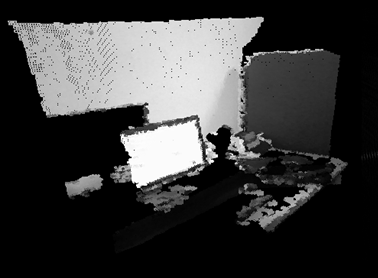
\includegraphics[width=6cm]{images/methodology/FVR/capFrameOriginal}
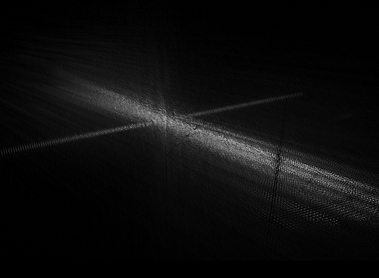
\includegraphics[width=6cm]{images/methodology/FVR/capFrameMagFFT}
\caption{Left: Captured 3D frame, Right: Magnitude values in the frequency domain of the captured 3D frame}
\label{fig:FrequencyDomainExample}
\end{figure}
 
The 3D Fourier transform transforms a volume from the 3D spatial domain into the 3D frequency domain (see figure \ref{fig:FrequencyDomainExample}). The frequency domain is a complex valued volume made up of sinusoids. Each voxel in the frequency domain represents the magnitude, phase and direction of a wave. These properties are important for computing camera pose as shall be discussed upcoming sections. An efficient software implementation of the Fourier transform named the Fast Fourier Transform (FFT) is able to compute the frequency domain given N-dimensional data. \\

Exploiting the properties of the FFT and the frequency domain, cross correlation may be carried out efficiently in order to compute the optimal camera location change between frames. As in the 2D approach, this algorithm is named phase correlation and is a popular approach in 2D image processing to align two images. Applied to two 3D frames captured by sensors (or partially generated via software) it may also be used to register the frames for 3D reconstruction as well as compute the translation part of the camera pose change for SLAM algorithms. This procedure is defined here as a function named $PhaseCorrelation$ (Eq. \ref{eqn:PC_basic}). This function takes two frames (3D volumes) as input and returns the best translation alignment between them in terms of maximizing correlation.  \\

\begin{equation} \label{eqn:PC_basic}
T(x, y, z) = PhaseCorrelation(V_x, V_y)
\end{equation}

The $PhaseCorrelation$ consists of 4 steps. In the first step the two captured 3D frames $V_1$ and $V_2$ are transformed into the frequency domain using the Fast Fourier Transform. This computes two new volumes $F_{1_{x,y,z}} = FFT(V_1)$ and $F_{2_{x,y,z}} = FFT(V_2)$. Applying the Fourier Shift Theorem to the context of camera pose estimation, if frames $V_1$ and $V_2$ are separated by some camera translation, then $F_{1_{x,y,z}}$ and $F_{2_{x,y,z}}$ will have phase values shifted relative to each-other. The normalized cross power spectrum (equation \ref{eqn:PHCOR_eq}) of the two complex valued Fourier spaces may then be used to find the camera translation change. The normalized cross power spectrum of $F_{1_{x,y,z}}$ and $F_{2_{x,y,z}}$ is another complex valued volume of the same size. \\

\begin{equation} \label{eqn:PHCOR_eq}
F_{3_{x,y,z}} = \frac{F_{1_{x,y,z}} \circ F_{2_{x,y,z}}^*}{ | F_{1_{x,y,z}} \circ F_{2_{x,y,z}}^* | }
\end{equation}

In equation \ref{eqn:PHCOR_eq}, $\circ$ is an element-wise multiplication and $|x|$ is the magnitude function or absolute value function. The Inverse Fast Fourier Transform ($IFFT$, $FFT^{-1}$) may then be used on the output of the normalized cross power spectrum volume to produce a phase correlation surface. The peak value on the phase correlation surface represents the optimal value of the correlation function applied to the two original real valued 3D frames. Therefore the $PhaseCorrelation$ procedure is equivalent to the cross correlation procedure, but rather than being complexity $N^6$, phase correlation reduces the complexity to approximately $6N^3 \times Log(N)$. \\


Due to the nature of camera capture, if the camera is translated by some vector before the capture of the next frame. Then the first frame contains data which the second frame does not, conversely, the second frame will capture some other data which is not present in the first frame (unless the camera was not moved). The parts of the 3D frames which do not overlap cause noise on the phase correlation surface. This makes it more difficult to decipher the location of the peak. There may be several peaks to choose from, or no clear peak. The nature of computing the Discrete Fourier Transform also affects this. The Discrete Fourier Transform assumes the output Fourier space is an infinitely repeating signal. The cross correlation procedure on the other hand does not assume this, so therefore the phase correlation surface may be affected. The solution adopted by many is to filter the volumes prior to transforming into the frequency domain. This can be done using a Hanning window function (equation \ref{eqn:HanningFunction}). This function can be used to filter edge effects prior to computing the Fourier transform which helps to reduce noise on the phase correlation surface. \\

\begin{equation} \label{eqn:HanningFunction}
Hanning(x) = \frac{1}{2}(1 - cos\left(\frac{2\pi x}{\frac{N}{2} - 1}\right)
\end{equation}

Noise on the phase correlation surface may also be present if other types of transforms are. In this case, the true camera translation may be lost. Therefore, camera pose/rotation must be computed prior to computing the camera translation. Other artefacts which may produce noise on the phase correlation surface include moving objects. If an object is present in one scene and not the other, it will cause some noise to be present in the phase correlation surface, making finding the peak more difficult but not impossible. Alternatively if there is an object whose location is changed between frames, the same thing may happen. The phase correlation procedure should be robust to these artefacts already but filtering approaches may also prove useful in selecting the correct peak which optimizes the translation used to register the 3D camera frames. \\

\subsubsection{Camera Rotation and Zooming}
\label{Sec:RoteZoomingSection}
SLAM and 3D reconstruction algorithms must compute both the camera location changes as well as camera pose. SLAM must compute this pose to track the camera, 3D reconstruction methods may simply register the data for integration or compute the camera pose prior to alignment and integration. Computing this involves estimating the camera's post change (rotation) from one frame to another. This may take the form of a $4 \times 4$ rotation matrix or the explicit magnitudes of rotation for each axis in a pre-determined order. These two formats may be converted between each other. The pose may also be represented by three axes (three orthogonal vectors) which represent the coordinate space of the camera. \\

Another transform not covered often in 3D reconstruction literature is that of scale. Given a single camera moving in a 3D space, scale is of no concern. However, if frames are zoomed or data is computed across sensors, scale factors may be unknown. For example, if an RGB-D image is captured as frame 1 and a second is captured as frame 2, but frame 2 is zoomed (scaled) prior to projection then the data may still be registered if scale may also be recovered. Alternatively if frame 2 is captured by another sensor or software system and is projected at a different scale, then this scale should also be recovered. The recovery of scale could be considered most important in the case of monocular 3D reconstruction. Here, the fundamental matrix may be used to calibrate camera frames. Once calibrated, stereo methods may be used to extract dense depth information for each frame. The problem with this technique is that depth is relative but not to scale across multiple frames. If the scale could also be recovered during the camera pose estimation procedure it would eliminate the need for more advanced methods of optimization. \\ 

Phase correlation alone cannot register against camera rotation. An important part of SLAM is the ability to recover 3D camera pose, and a fundamental part of 3D reconstruction is to align dense depth data against as many camera movements as possible. Therefore we propose using an extension of the popular rotation and scale recovery procedure from 2D registration research to perform camera rotation change estimation as well as align frames which have been zoomed or scaled to fit the volumetric space. \\

Using this technique, which is comprised of a few spatial transformations and phase correlation, a single axis of rotation may be recovered. The axis chosen is integrated into the spatial transformation part of the procedure. Since most scenes would be captured by moving around a room and rotating the camera to look at the areas within the scene directly around the user and camera, we have designated the y-axis of rotation as the most important axis to recover. Additionally, vehicles (with dash mounted cameras) and robots typically keep the camera steady and perform movements and rotations about the y-axis. This technique's application to 3D reconstruction is novel in itself, but a completely novel technique named FVR3D is presented in this work for recovering all 3 axes of rotation using Fourier techniques, this is discussed in section \ref{FullRecovery3DSection}. FVR3D makes use of the rotation and scale estimation procedure discussed here.  \\


Given two frames captured as 3D volumes, $V_1$ and $V_2$, where $V_2$ is captured by a second camera at a different location, pose (about the y-axis) and has data projected differently prior to both systems submitting data for registration and integration into a single global 3D reconstruction. From the perspective a registration system, the data in frame 2 has been transformed by translation vector $t = [t_x, t_y, t_z]$, rotation factor $\theta$ and scale $\varphi$. The procedure to recover these values makes use of several properties of the Fourier transform and the frequency domain. One important property is that, the magnitude of the frequency domains of both $V_1$ and $V_2$ are related differently to the raw data from the frames alone. The magnitudes are related by the same rotation factor $\theta$ and scale factor$\varphi$, but these transforms occur about the origin at the center of the magnitude volumes, rather than at locations which depend on the translation factor $t$. In this way, the translation factor can be ignored and the rotation and scale factors can be recovered separately. \\


\begin{figure}[!htb]
\centering
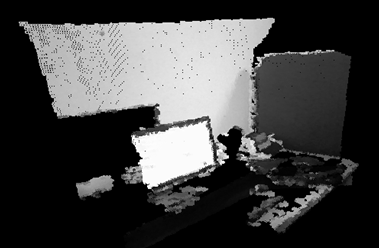
\includegraphics[width=6cm]{images/methodology/FVR/capFrameA}
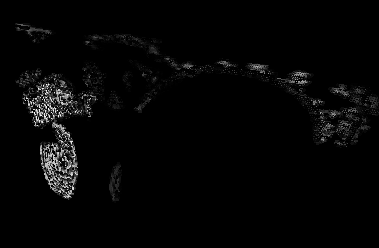
\includegraphics[width=6cm]{images/methodology/FVR/capFrameLogPolar}
\caption{Left: Captured 3D frame, Right: Log-Polar Transform of the captured 3D frame}
\label{fig:LogPolarTransform3DExample}
\end{figure}

This procedure recovers the camera rotation as well as any scale factor which may be present independent to any translation effects. Therefore, once the rotation and scale factors have been recovered, the translation parameters may be estimated using the 3D phase correlation procedure described in section \ref{sec:PCForSLAM} as an additional step. This procedure starts by applying a Hanning windowing function to both volume frames. As mentioned the Hanning window function is used to counter the noise generated by the Fourier transform. This noise occurs because the discrete frequency domain is assumed to be infinity repeating when in practical computer algorithms the space is treated as singular occurring structure surrounded by finite empty space. This unavoidable assumption makes some operations on the frequency domain erroneous. The function for the Hanning window was given in equation \ref{eqn:HanningFunction}, the scalar for each voxel in frames may be computed for each point $[x,y,z]^T$ via equation \ref{eqn:Hann}. The use of this filtering is especially important in computing the rotation and scale parameters. \\


\begin{equation} \label{eqn:Hann}
\scriptstyle
HW_{x,y,z} = \frac{1}{2}\left(
1 - cos \left(
\frac{2\pi
\left(
\sqrt{\left(\frac{N}{2}\right)^3} -
\sqrt{
\left(x-\frac{N}{2}\right)^2 + \left(y-\frac{N}{2}\right)^2 + \left(z-\frac{N}{2}\right)^2
}
\right)
}
{2\sqrt{\left(\frac{N}{2}\right)^3} - 1}
\right)
\right)
\end{equation}

The translation separating the camera frames must be removed from the equation prior to estimating the rotation and scale. As mentioned, the magnitude of the frequency domain is independent to the effects of translation. So, the magnitude of the frequency domains of both frames are taken, $M_1 = |FFT(V_1)|$, $M_2 = |FFT(V_2)|$. The zero frequency, which is at the corners of the volume (because the discrete frequency domain is assumed to be circularly repeating infinitely) must be transformed to the center of the volume. In this way, any rotation or scaling occurs about the center of the volume. Then, both $M_1$ and $M_2$ are filtered using an element-wise log function. The frequency domain contains larger values around the zero mean and low frequency areas and smaller values around the higher frequency areas, but for the purposes of computing the camera rotation and any possible scale factor, all frequencies should be treated equally. The element-wise log function therefore suppresses the lower frequency values bringing the higher frequencies up to a similar level. \\

Given these new volumes, $M'_1 = Log(M_1)$, $M'_2 = Log(M_2)$, a geometric transform named the log-spherical transform is used on both $M'_1$ and $M'_2$. The log-spherical transform function re-arranges the input data in such a way, that any y-axis rotation becomes x-axis translation and any scaling becomes z-axis translation. Equation \ref{eqn:Log_Spherical} shows the log-spherical space coordinate $(X_{log-spherical}, Y_{log-spherical}, Z_{log-spherical})$ for a given $(x,y,z)$ euclidean space coordinate. This encompasses the effects of the log-spherical transform. \\


The output x coordinate, $X_{log-spherical}$ in the log-spherical transform centers the input x and y coordinates about the centre of the volume and uses the atan trigonometric function to obtain the angle in degrees the point is around the y-axis. This is scaled to the full size of the volume via scalar $\frac{N}{360}$. The result is that data at different angles about the y-axis are grouped by their particular angle linearly along the output x-axis. The output y coordinate $Y_{log-spherical}$ is also centered about the volume center and is put through the cosine function. This gives the angle in degrees about the secondary axis (x rotational axis). The degree between 0 and 180 is then mapped to the range $[0-N]$ using the scalar $\frac{N}{180}$. The y coordinate can be passed to the cosine function directly because it is known that the x rotational angle can be computed as the cosine function of the dot product between the input point, $[x,y,z]^T$ and the vertical axis $[0,1,0]^T$ which results in $x \times 0 + y \times 1 + z \times 0 = y$. \\

The output z, $Z_{log-spherical}$ coordinates encompasses the scale information of the input coordinate. First the distance between the input coordinate and the center of the volume is computed. This is placed through a log function, the log function compresses the distance such that any scaling relationship between distances becomes a relationship of addition, or in this case volume translation along the z-axis. This is then mapped using the scalar $\frac{N}{log\left(\frac{N}{2.56}\right)}$. This mapping is used so that scales within the range $[2.56^{-1}, 2.56]$ may be registered. Increasing this range too much results in decreased precision and possibly a decrease in accuracy or an inconclusive registration result. \\


\begin{equation} \label{eqn:Log_Spherical}
\begin{split}
X_{log-spherical} & = \frac{atan\left(
\left( x-\frac{N}{2} \right) \times
\left(y-\frac{N}{2}\right)^{-1}
\right)N}{360}\\
Y_{log-spherical} & = \frac{acos\left(
y-\frac{N}{2}
\right)N}
{180} \\
Z_{log-spherical} & =\frac{log\left(
\sqrt{\left(x-\frac{N}{2}\right)^2+\left(y-\frac{N}{2}\right)^2+\left(z-\frac{N}{2}\right)^2}
\right)N}{log\left( \frac{N}{2.56} \right)} \\
\end{split}
\end{equation}

The log-spherical transforms of $M'_1$ and $M'_2$ are then related by translation. The translation relationship describes the camera rotation and the scale factor separating both of the original frames. The exact translational differences can easily be recovered using phase correlation. The resulting peak location from the phase correlation procedure, $(x_{M'},y_{M'},z_{M'}) = PhaseCorrelation(M'_1, M'_2)$ is used to estimate the rotation and the scale. The phase correlation surface of these two volumes is often very noisy. It is usually noisier than phase correlating data from the spatial domain. Filtering techniques may be used to alleviate this issue. If multiple peaks are detected, the rotation and scale may also be tested for each candidate peak. The rotation $\theta$ and scale factor $\varphi$ separating the two original frames, $V_1$ and $V_2$ can then be computed using the peak values on the phase correlation surface, $(x_{M'},y_{M'},z_{M'})$. The functions to compute $\theta$ and $\varphi$ are given in equation \ref{eqn:ROTATIONSCALEFROMXM}. \\
 
\begin{equation} \label{eqn:ROTATIONSCALEFROMXM}
\begin{split}
\theta & = \frac{-360x_{M'}}{N}\\
\varphi & = e^{
-\left(
2.56^{-1}N
\right)z_{M'}N^{-1}
}
\end{split}
\end{equation}

The $(x_{M'}$ coordinate is mapped to a unit number in the range $[0,1]$ and is scaled by $-360$ resulting in $\theta$, the angle of rotation which may be used to align the frames. The $z_{M'}$ coordinate is also mapped to a unit number, it is then scaled by $\frac{N}{256}$ in order to align the result prior to inverting the log function effects. The value is negated also, this gives the relationship relative to frame 1 rather than frame 2. Finally, the log function is reversed using the exponential function. The resulting rotation matrix may be formed as in equation \ref{eqn:RoteRegMatrix}. This conjuncted matrix first transforms the center of the volume to the origin and then rotates it by $\theta$, then transforms it back to the center of the volume. \\

\begin{equation} \label{eqn:RoteRegMatrix}
\left[
\begin{array}{cccc}
1 & 0 & 0 & \frac{N}{2} \\
0 & 1 & 0 & \frac{N}{2} \\
0 & 0 & 1 & \frac{N}{2} \\
0 & 0 & 0 & 1 \\
\end{array}
\right] \times
\left[
\begin{array}{cccc}
cos(\theta) & 0 & sin(\theta) & 0 \\
0 & 1 & 0 & 0 \\
-sin(\theta) & 0 & cos(\theta) & 0 \\
0 & 0 & 0 & 1 \\
\end{array}
\right] \times
\left[
\begin{array}{cccc}
1 & 0 & 0 & -\frac{N}{2} \\
0 & 1 & 0 & -\frac{N}{2} \\
0 & 0 & 1 & -\frac{N}{2} \\
0 & 0 & 0 & 1 \\
\end{array}
\right]
\end{equation}

The resulting scaling matrix is formed similarly (equation \ref{eqn:ScaleRegMatrix}) by transforming the volume center to the origin, scaling the geometry and then transforming the data back to the center of the volume. The resulting matrix to un-do both the scale and rotational effects of the camera movement can therefore be computed as the scale matrix multiplied by the rotational matrix, $SR_{matrix} = S_{matrix} \times R_{matrix}$. \\

\begin{equation} \label{eqn:ScaleRegMatrix}
\left[
\begin{array}{cccc}
1 & 0 & 0 & \frac{N}{2} \\
0 & 1 & 0 & \frac{N}{2} \\
0 & 0 & 1 & \frac{N}{2} \\
0 & 0 & 0 & 1 \\
\end{array}
\right] \times
\left[
\begin{array}{cccc}
\varphi & 0 & 0 & 0 \\
0 & \varphi & 0 & 0 \\
0 & 0 & \varphi & 0 \\
0 & 0 & 0 & 1 \\
\end{array}
\right] \times
\left[
\begin{array}{cccc}
1 & 0 & 0 & -\frac{N}{2} \\
0 & 1 & 0 & -\frac{N}{2} \\
0 & 0 & 1 & -\frac{N}{2} \\
0 & 0 & 0 & 1 \\
\end{array}
\right]
\end{equation}

If frame 1, $V_1$ is then transformed by scale-rotation matrix $SR_{matrix}$, the resulting volumes are separated only by translation. The translation matrix separating them may then be computed using phase correlation. The result of this procedure is that the rotation factor $\theta$, the scale factor $\varphi$ and the translation factors $x$, $y$ \& $z$ have all been recovered. Given the translation matrix $T$ formed by the translation factors $x$, $y$ \& $z$, the full registration matrix aligning frames $V_1$ and $V_2$ may be computed as, $M_{T,\varphi,\theta} = T \times SR_{matrix}$. $M_{T,\varphi,\theta}$. This matrix can be used to align frame 1 to frame 2 prior to integration. Alternatively frame 2 may be aligned with frame 1 by transforming it by $M_{T,\varphi,\theta}^{-1}$. \\

The camera pose relationship between frame 1 and frame 2 is also now known. Given the camera coordinate axes in frame 1, $Forward \in R^3$, $Right \in R^3$, $Up \in R^3$ the coordinate space for the camera in frame 2 may be computed by adjusting these axes by the registration matrix $M_{T,\varphi,\theta}$. Once the camera pose is known, the camera may be tracked by repeating the process between successive frames, the resulting dense 3D data may then be integrated to create the complete 3D reconstruction. Alternatively, the dense 3D data may be projected and integrated directly resulting in the output 3D reconstruction. \\

\subsubsection{Conclusion}

In this section, the volume registration method is applied to 3D pose estimation. In the next section this is extended into a full 3D reconstruction algorithm. Experiments in sections \ref{Sec:FVRSOTA,Sec:CamTransTrackExp}
show that this method is capable of reconstructing scenes accurately using different sensors whilst being robust to noise. 

\section{Fourier Volume Reconstruction}

Section \ref{Sec:VolumeRegistrationSection} described techniques to register camera frames which have been projected to three dimensions. As mentioned, these frames may be registered with respect to the most common type of camera pose transform, y-axis rotation, as well as camera movement. In addition, scale may be registered. For frames which have been projected differently or frames in which depth is computed relative to each frame, such as per frame depth computed in monocular view situations, scale is an important transformation to register against. This is especially true since most existing methods perform simple rigid movement camera pose registration. \\

This section integrates the phase correlation method into a full 3D reconstruction algorithm named Fourier Volume Registration (FVR). This algorithm may also be used to perform SLAM and it may be applied to input data in which depth is not projected at correct scale between frames. The input required for this method is a list of colour RGB images, each with a depth component. The data may be generated via an RGB-D active camera or computed implicitly using a stereo camera set-up or calibrated monocular set-up. \\

Results for the FVR method are presented in sections \ref{StereoSOTA}, \ref{ActiveSOTA}, \ref{Sec:MonocularSOTA} and \ref{Sec:CamTransTrackExp} and show the FVR method is capable of accurate 3D reconstructions whilst being robust to noise. In some experiments, it also outperforms the current state-of-the-art methods from the literature. Details on how the Fourier Registration methods described in section \ref{FVRSectionA} are integrated to create the FVR algorithm are presented in the following sections. \\


\subsubsection{Pipeline}

\label{sec:FVRPipelineSect}

In Figure \ref{fig:PIPELINENo1} a pipeline for the FVR registration method is shown. This is a high-level pipeline for the recovery of scale, y-axis rotation and translation. Many of the operations may be performed using GPU processing techniques. Signal Processing methods are very common, many hardware devices exist which can execute these algorithms which are used by the FVR method. \\

Two volumes, $Volume_1$ and $Volume_2$ are both first put through a Hanning window function, these operations may be performed in parallel. This process multiples each voxel by a scalar which may be computed entirely based on location or a 3D lookup table. Each Hanning window operation may also be performed on the GPU or using another parallel programming technique such as multi-threading. \\

Next, using the FFT the magnitude of the Discrete Fourier Transform is computed. The 3D FFT is a common operation which is implemented on most General Purpose Graphics Processing Units (GPGPUs). The 3D FFT operations on the GPGPUs produce the real and imaginary components of the frequency domain, but an additional GPU operation may be used to compute the magnitude values based on the real and imaginary values. Again this operation is easily extended to parallel processing platforms and both volumes may be transformed in parallel. \\

The $Log(x)$ function is also a per voxel operation which may be computed in a parallel processing platform and both volumes may be transformed in parallel. The log-spherical transform may be computed for each volume at the same time and is also inherently parallel. Additional memory requirements must also be met as both input and output volumes must be simultaneously kept in memory. \\

\begin{figure*}[!htb]
\centering
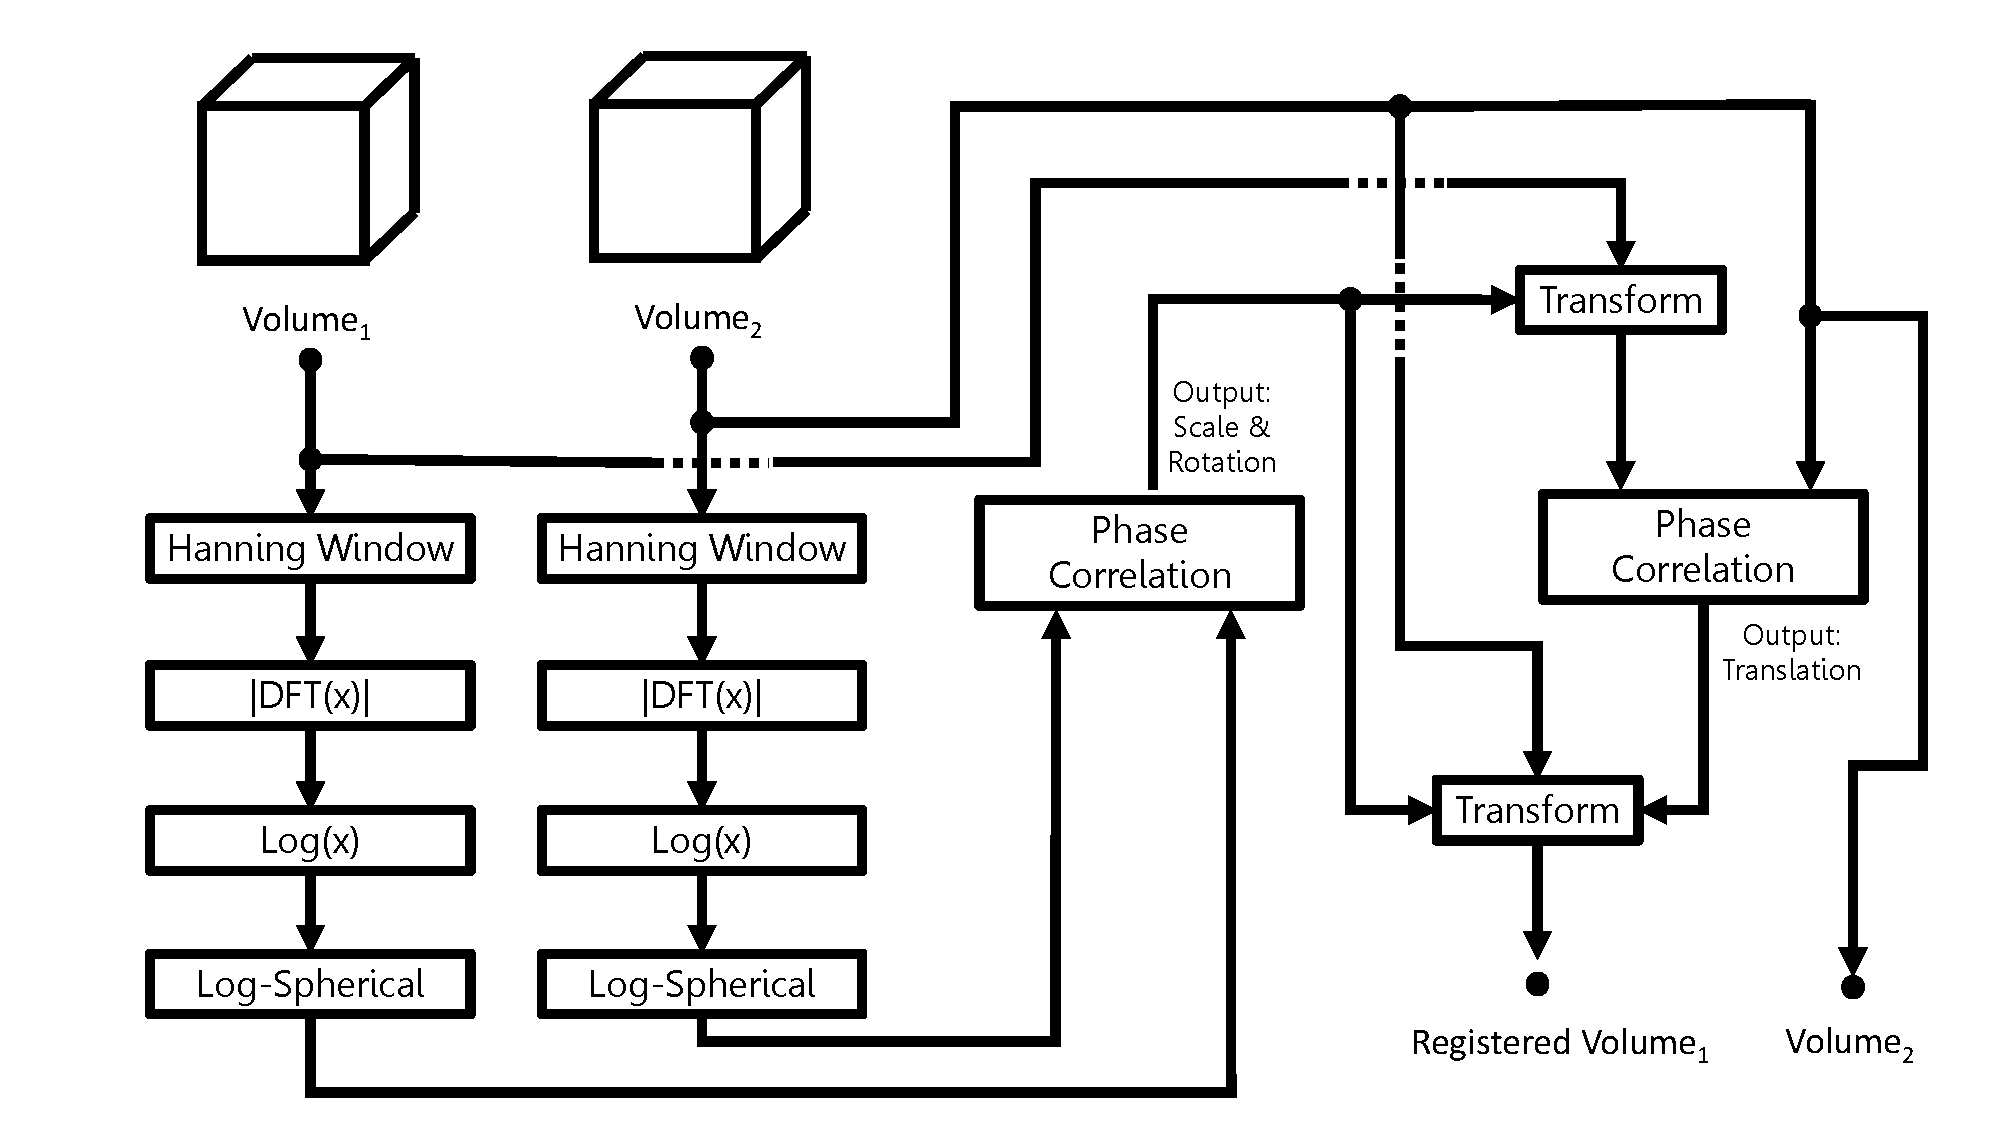
\includegraphics[width=5.0in]{images/ch2/pipeline2}
\caption{System Diagram for Registration Process}
\label{fig:PIPELINENo1}
\end{figure*}


The phase correlation operation is made up of multiple FFTs and their inverse, as well as computing the cross power spectrum between two volumes. All these operations may be performed on GPGPUs. Searching for the output peak is, however, a sequential process. Parallel techniques, such as reduction, may be used but the performance gain is minimal for volumes of size $256^3$. \\

Transforming the input volume is another process which may be performed using parallel techniques. The final phase correlation procedure is also parallel in nature apart from the peak value search on the phase correlation surface which is a sequential process. \\



\subsubsection{Algorithm}

Using the registration pipeline to compute the relationship between two frames, a SLAM and 3D reconstruction algorithm may be formulated. This algorithm can construct dense 3D reconstructions whilst simultaneously computing relative camera pose estimates. \\

 
The overall algorithm is presented in Listings \ref{algorithm:PCSLAMNo1}. In the first line, the first frame is read as an RGB-D image into variable $f_1$. This RGB-D image is projected into a 3D point cloud representation using a projection function. The point cloud data for this first frame is then integrated into an automatically expanding occupancy grid representing the global 3D reconstruction output variable named $GlobalReconstruction$. \\

An accumulation matrix, $M$, is used to formulate transforms for each frame read in. It is used by the algorithm to integrate frames directly into the output global reconstruction. Two variables, $Camera_{location}$ and $Camera_{pose}$, are used to represent the camera location and pose information. The pose contains three vectors representing the camera space within the world space. A list of the camera locations and poses is referred to by the $Cameras$ variable. Each element in this list is a camera location and pose pair. \\

\begin{figure}
\begin{lstlisting}[language=c++,caption=Phase Correlation Based SLAM Algorithm,label=algorithm:PCSLAMNo1,mathescape,basicstyle=\ttfamily]
$f_1$ = ReadFrame();
$PointCloud$ = project($f_1$);
$GlobalReconstruction$.integrate($PointCloud$)
$M$ = IdentityMatrix();
$Camera_{location}$ = $[0, 0, 0]^T$;
$Camera_{pose}$ = $[[1, 0, 0]^T,[0, 1, 0]^T,[0, 0, 1]^T]$;
$Cameras$ = $\left[\left[Camera_{location}, Camera_{pose}\right] \right]$;
while(more frames){
	$f_2$ = ReadFrame();
	$points_1$ = project($f_2$);
	$points_2$ = project($f_1$);
	$V_1$ = Voxelize($points_1$);
	$V_2$ = Voxelize($points_2$);
	$(\theta, \varphi, t_x, t_y, t_z) = VR_{\theta \varphi t_x t_y t_z}(V_1, V_2)$;
	$Temp = $TransformMat($(\theta, \varphi, t_x, t_y, t_z)$);
	$M = M \times Temp$;
	$points_1$ = Transform($points_1$, $M$);
	$GlobalReconstruction$.integrate($points_1$);
	$Camera_{location}$ = $Temp^{-1} \times Camera_{location}$;
	$Camera_{pose}$ = $Temp^{-1} \times (Camera_{pose} + Camera_{location})$;
	$Camera_{pose}$ = $\frac{Camera_{pose} - Camera_{location}}{Camera_{pose} - Camera_{location}}$;
	$Cameras.add(\left[Camera_{location}, Camera_{pose}\right])$;
	$f_1$ = $f_2$;
}
\end{lstlisting}
\end{figure}

The algorithm iterates over each frame pair which must be registered and integrated. Each iteration begins by reading in a new frame. This is pointed to by variable $f_2$. Next, both $f_1$ and $f_2$ are projected into point clouds named $points_1$ and $points_2$ respectively. The Fourier Volume Reconstruction method requires the frames be integrated into 3D volumes, so the Voxelize function is used to integrate the points and colour information into volumes. \\

The FVR method works with either integrated greyscale information based on the RGB data, or with raw binary occupancy values. The use of RGB data may have slight performance implications. Many computer vision algorithms prefer to work in greyscale, especially feature matching methods. This is often due to a combination of complexity and performance reasons. Whilst colour information does improve accuracy, it is considered to be minimal relative to savings made in terms of computational complexity by processing greyscale data alone. \\

Integrating the colour information for use in the FVR method does not incur any performance penalty. The only shortcoming of using the extra colour information to increase accuracy is the loss of the ability to work in total darkness using RGB-D sensors. \\

As mentioned in the literature, the Kinect Fusion technique only makes use of depth information which is obtained via an active camera (the Kinect). In this way it can effectively work in the dark. If the FVR method uses colour information integrated directly, and the colour components do not pick up any light, the method will fail. Whether or not colour information is present can be easily detected and because FVR also works by simply registering occupancy volumes, it can switch over to this method upon detecting that no colour (visible light) information is available. \\

Once the volumes are reconstructed, the rotation, scale and translation factors may be computed using the pipeline discussed in section \ref{sec:FVRPipelineSect}. A transformation matrix, $Temp$, may then be created from these values. Such a matrix was presented in section \ref{FVRSectionA}. $M$ is then replaced by itself multiplied by the computed transformation matrix $Temp$. In this way, $M$ can be used to accumulate previous registrations. \\

The $points_1$ point cloud is then transformed by the newly computed $M$. The point cloud can then be integrated into the global reconstruction. Next, the camera location and pose list must be updated. The camera location is adjusted by the inverse of the newly computed $Temp$ matrix. As previously mentioned, the camera transforms will be inversely related to the registration transforms. \\

The camera pose is also updated, by adjusting the axes relative to the camera location using the $Temp$ matrix. The camera pose vectors are then normalized and added into the list of camera locations and poses. Finally, $f_1$ is set to $f_2$. In this way, the algorithm can repeat with $f_1$ as the previous input frame. \\  



\subsubsection{Integration}

The integration procedure used with this technique is the common global voxel integration method. An automatically expanding volume is used to store the global 3D reconstruction. Given the algorithm described above, the output global reconstructed volume must take in point cloud data, and integrate it into the volume. \\

The algorithm proposed does not make use of loop closure. Many recent techniques also forgo the use of this procedure, especially if they integrate globally. The FVR method can also be easily adjusted by changing the last line of the algorithm. Rather than simply setting $f_1$ to $f_2$, $f_1$ may be set to the volume extracted by sampling the global reconstruction into a volume based on the most recent camera location and pose computed. This way, loops may be detected by registering upcoming frames globally. \\


\subsubsection{Limitations}

The FVR method is capable of registering 3D pose data and in turn can generate accurate, high quality 3D reconstructions. However, it is limited to a single axis of rotation (the y-axis). The FVR method was tested and remains robust to up to 10 degrees of rotation along the other axes, but it is still not able to register all 3 axes of rotation. To move past this limitation whilst retaining the robustness and accuracy of the technique, a novel extension named FVR-3D is proposed in section \ref{FullRecovery3DSection}. Both the FVR method and the FVR-3D algorithm are tested empirically in Chapter \ref{ch:Experiments} and results show they outperform other algorithms from the literature in terms of 3D pose estimation and 3D reconstruction. \\
\section{Monocular FVR}

During experiments, it was found that MVVR (FVR applied to monocular camera sensor data) had considerably less accuracy and robustness than the other FVR methods (FVR, FFVR and FVR-3D). Additionally, we found that MVVR was less robust to rotational transforms. This is due to the fact that depth maps produced by monocular sensor methods, such as optical flow, do not produce sufficiently accurate and reliable depth maps. Results from stereo and active camera tests suggest that this is due to the reduction in accurate and precise depth data generation. \\

Nevertheless, to evaluate the performance of the MVVR method, quantitative experiments were performed on the Kitti Vision Benchmark Data Set. In these experiments, the MVVR method was compared with methods from the literature including FM2D, FM3D. ICP and PCA. Each depth map was projected into volume sizes of $256^3$ for processing by the rest of the MVVR method (the FVR part). To generate the depth maps, a local 2D block matching method was used. Kernel sizes used in the correlation procedure were $3 \times 3$ in size with a search area size of $21 \times 21$. The sizes of the kernel, search area and volume sizes were all chosen empirically. \\

Depth maps computed using the block matching method are only estimates of true scene depth. Therefore, resulting projections are not accurate. These projections, however, are still good enough to produce reconstructions. Registration of these inaccurate projections is difficult due to the amount of noise in the data. Figure \ref{fig:lidarVSMono} shows the noise contrast between depth maps produced by a LIDAR and a monocular block-matching system. \\

\begin{figure}[!htb]
\centering
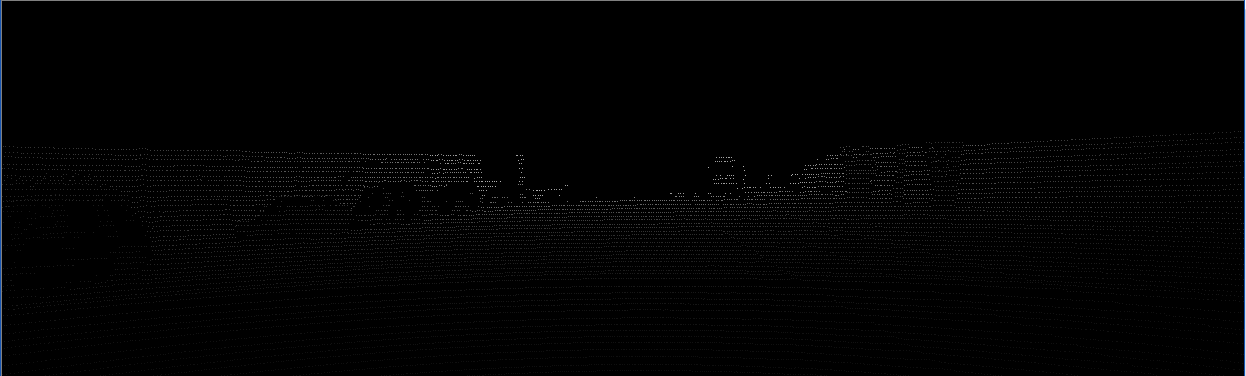
\includegraphics[width=2.9in]{images/methodology/FVR/mono/color}
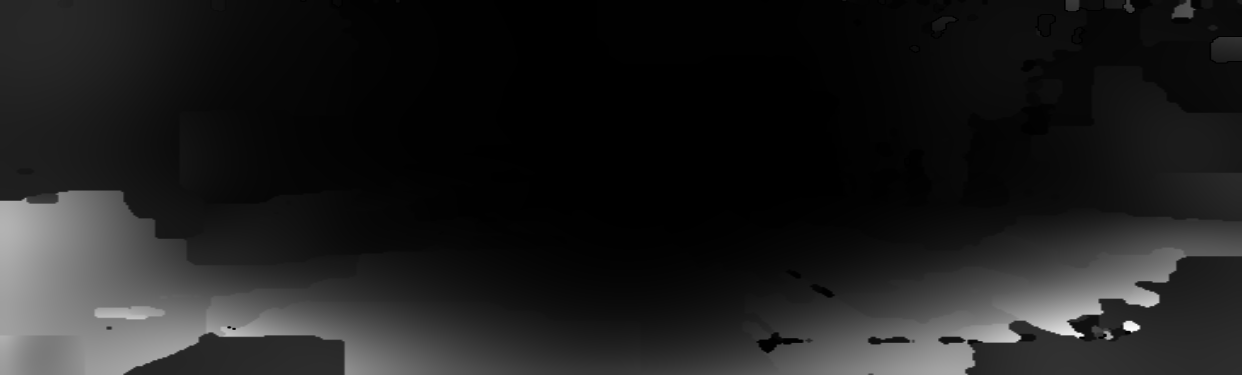
\includegraphics[width=2.9in]{images/methodology/FVR/mono/depth}
\caption{Left: Ground Truth Depth Map Computed Using a LIDAR System, Right: Depth Map Computed Using a Monocular Method}
\label{fig:lidarVSMono}
\end{figure}


Results on the Kitti Benchmark 0001 Sync data set are shown in Table \ref{table:MVVRQuantitativeExperimentResults}. In these results, ICP outperformed the other methods, with each algorithm having larger errors due to the inaccurate depth maps. Here, FVR achieved the best result ~29.25 \% of the time. Compared to results in Table \ref{tab:kittidata0001sync}, the MVVR method was less competitive than ICP. Due to the low-quality projections, FM2D and PCA failed were not able to register every frame. Most of the algorithms had incorrectly registered frames at some point.

\begin{table}[t]
\centering
\caption{Reconstruction Errors for the Kitti Data 0001 Sync Data Set Using Monocular (RGB) Input Only}
\begin{tabular}{ccc}
\hline
\textbf{Algorithm} & \textbf{Median Error $\times$ 1000} & \textbf{\% best results}\\ \hline
FM2D	& 3742.4 & 2.83\%\\
FM3D	& 918.05 & 14.15\%\\
ICP	& 772.48 & 50.94\%\\
PCA	& 2046.96 & 2.83\%\\
MVVR	& 944.81 & 29.25\%\\
\end{tabular}
\label{table:MVVRQuantitativeExperimentResults}
\end{table} 

These results, and those from the Stereo and Active camera experiments, indicate that, if the quality of the depth maps had been higher, the FVR based methods would have produced better results. \\

\section{Improving Efficiency in FVR}

The proposed FVR method is interesting in comparison with other major techniques such as Feature Matching + RANSAC, ICP and other optimization methods in that it is not an iterative method but is a closed form solution. That is, its computational complexity is fixed and does not depend on the input data. Despite this, some parts of the pipeline (see figure \ref{fig:PIPELINENo1}) remain intensive, even for GPGPU and other parallel processing devices. \\

In order to reduce complexity, the different parts of the pipeline were examined in order to reveal any possible improvements. It is understood that each Hanning window function in \ref{fig:PIPELINENo1} is required to reduce noise on the phase correlation surface. The technique is already highly parallelized    and is not very computationally intensive. Much effort has already been given to improving efficiency in computing the Fourier transform. \\

The element-wise log function is similar to the Hanning window function, it is required to correlate the data to find the rotation and scale factors separating both volumes. Furthermore it is already highly parallelized and cannot be simplified. The 3D phase correlation technique is by far the most computationally intensive operation within the pipeline. It requires 2 $\times$ FFTs, 1 $\times$ element-wise operation, 1 $\times$ inverse FFT and 1 $\times$ peak search operation. Moreover there are two required 3D Phase Correlation operations during the pipeline. The other transform operations are also element-wise operations introducing minimal computation expense into the pipeline. \\

In order to reduce the computational complexity of the 3D phase correlation, several projection operations are used to retain as much information as possible whilst reducing the data to 2 dimensions in such a way that 2D phase correlation (a much faster operation) may be used in place of 3D phase correlation to retrieve transformation factors. Two transforms are proposed to achieve this. The Spherical-Map Transform (section \ref{SMTransform} reduces the original 3D frames to 2D. One useful property of this transformation is that correlation between two Spherical-Map domains retrieved both two 3D frames yields the y-axis rotation and scale factor parameters between the original 3D frames. Moreover, because the spherical-map space is a 2D space, phase correlation may be used in place of manual correlation.  \\

The other transformation is proposed to efficiently compute translation factors separating two 3D volumes. This transform is simply named a projection transform (see section \ref{sec:PMTramsform}). It reduces the 3D input frames to 2D images whilst retaining the translational information along two remaining axes. Correlating two projection transform domain images yields two translation parameters (depending on the type of projection transform) which separate the two original 3D frames. \\

A block diagram integrating these speed improvements into the FVR method introduced in section \ref{FVRSectionA} is shown in figure \ref{fig:PIPELINE3}. This procedure is referred to as the Fast Fourier Volume Reconstruction method (FFVR). As shown in the block diagram, this procedure takes two 3D volume frames as input, $Volume_1$ and $Volume_2$. The second frame may be taken after the camera has changed pose about the y-axis and/or has moved locations. Both inputs are then put through a 3D FFT function to produce the magnitude values of the 3D frequency domain of both volumes. These operations may be performed on a GPGPU and may both be performed in parallel with each other. \\

The magnitude of the frequency domain is independent to translation and any rotation and scale occurs about the center of both volumes. Both frequency domain volumes are then transformed into 2D spherical space using the $Spherical2DMap$ function. This function produces an image in which 3D y-axis rotation from the original volume is interpreted as 2D translation. To recover the rotation parameter, phase correlation is used to measure the translational component separating the spherical-map domain images. This translational component is then processed to compute the y-axis rotational factor separating the original input volumes. The rotation factor be be directly output as a parameter if required. \\


\begin{figure}[!htb]
\centering
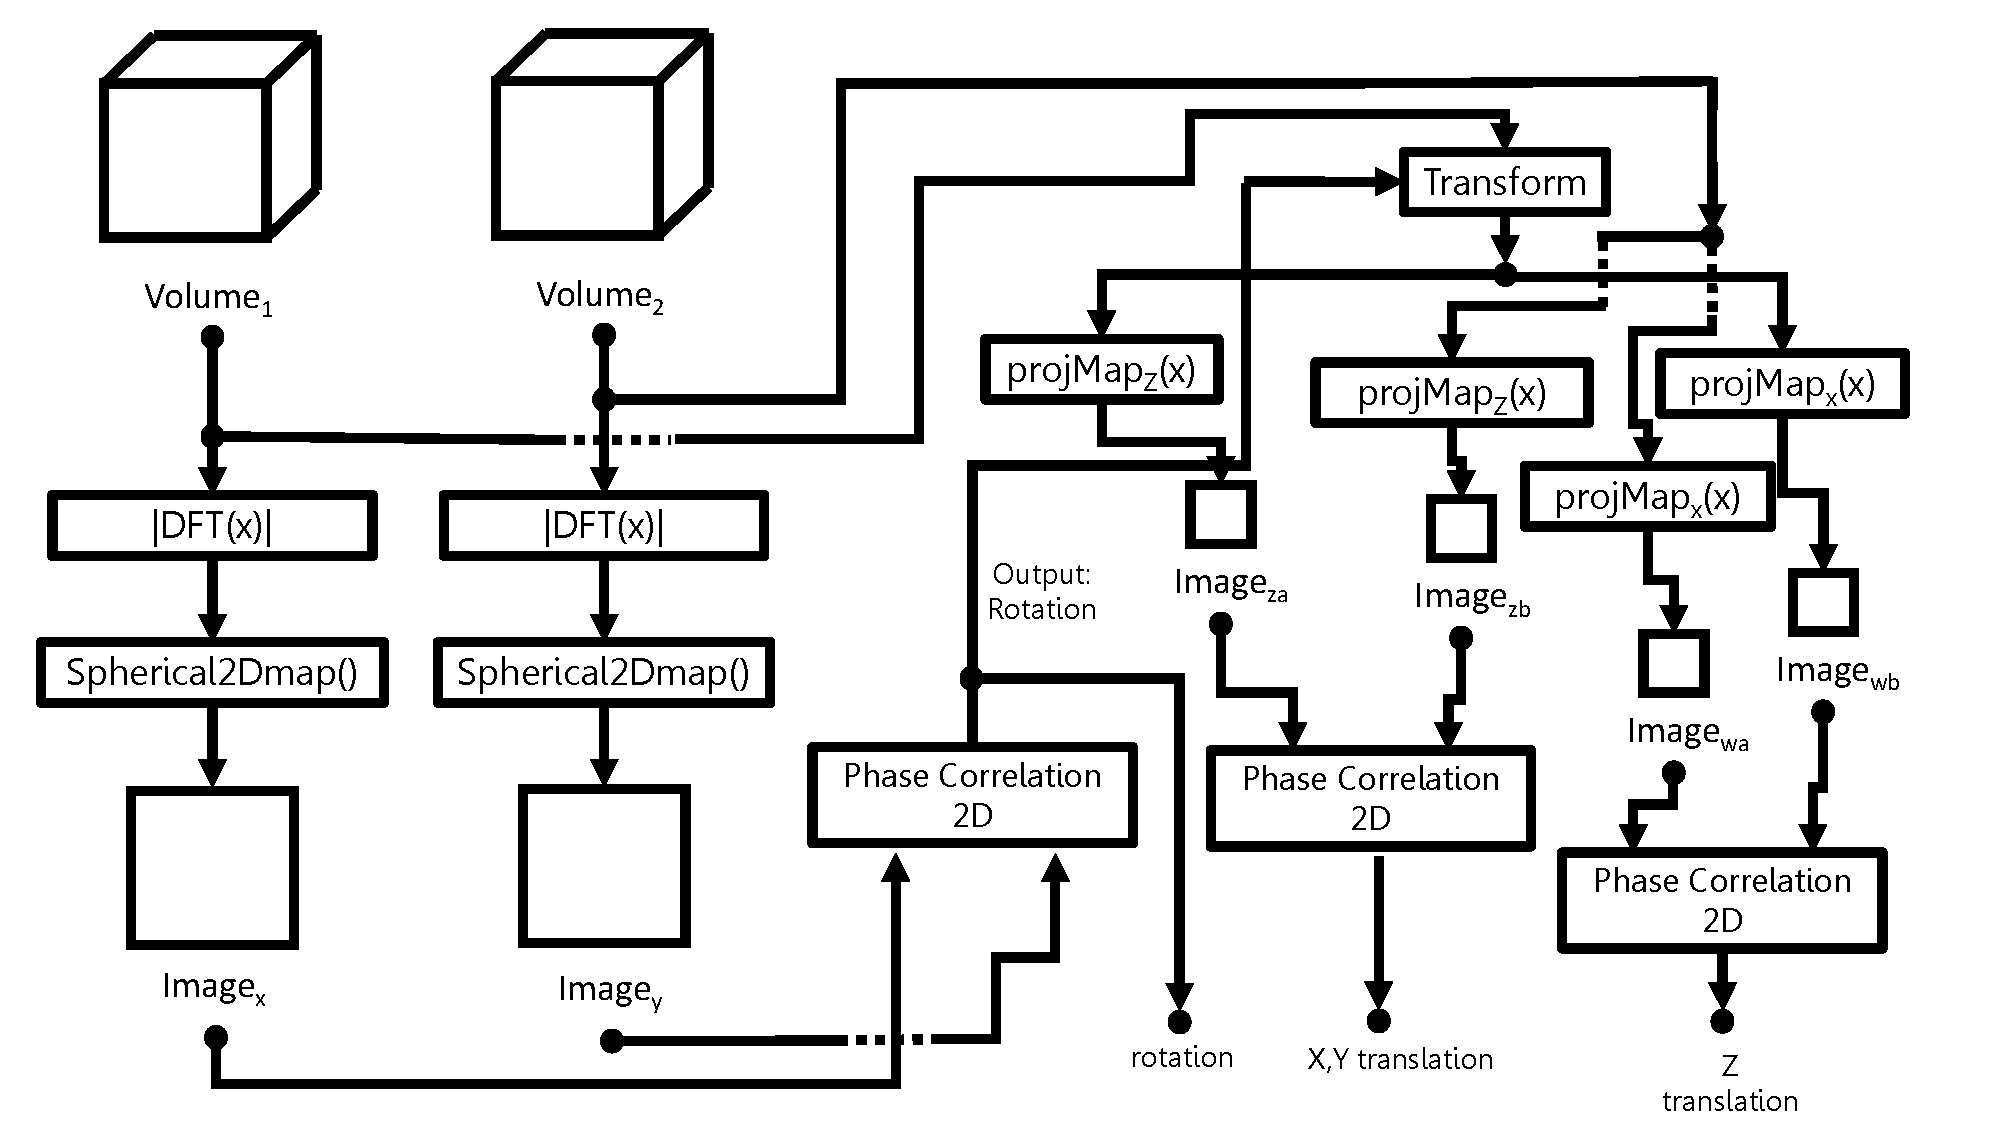
\includegraphics[width=5.0in]{images/ch2/pipeline3}
\caption{System Diagram for Fast Volume Registration}
\label{fig:PIPELINE3}
\end{figure}

Next, the first 3D frame, $Volume_1$ is transformed by the computed rotation factor. This leaves only a 3D translation transform separating both inputs $Volume_1$ and $Volume_2$. Two projection map transforms of both $Volume_1$ and $Volume_2$ (equivalent to 4 transforms in total) are then used to efficiently find this translation factor. The first projection map transform is along the z-axis. The z-axis projection map transform of $Volume_1$ produces 2D image, $Image_{za}$ the z-axis projection map transform of $Volume_2$ produces 2D image, $Image_{zb}$. Both $Image_{za}$ and $Image_{zb}$ may be phase correlated producing the x and y axis components of the translation separating $Volume_1$ and $Volume_2$. \\

The other two projection map transforms are along the x-axis. The projection map transform of $Volume_1$ produces $Image_{wa}$, whilst the projection map transform of $Volume_2$ produces $Image_{wb}$. These two images ($Image_{wa}$ and $Image_{wb}$) may be phase correlated producing the z-axis component of the translation. A composite registration matrix aligning $Volume_1$ to $Volume_2$ may be formed by translating each volume's center to the origin, rotating by the computed rotation factor, translating the origin to the volume's center and finally translating by the $[X,Y,Z]^T$ translation vector computed. \\

Noticeably, the Hanning window function and post $|DFT|(x)$ $Log(x)$ function from the original pipeline (figure \ref{fig:PIPELINENo1}) are missing. The Hanning window function may be incorporated in the first phase correlation procedure, which processes 2D images, therefore the Hanning window function would be in 2D rather than 3D which also improves efficiency as an entire dimension is removed from the process. The log function may also be performed as part of the phase correlation procedure, however it was found that the FFVR procedure estimates rotation more reliably using the spherical-transform if the log function is not performed. This saves additional computational power. \\

It is advantageous to use 2D phase correlation over 3D phase correlation from a computational complexity perspective. The 3D Fourier transform has complexity of $N^3 \times Log(N^3)$ whilst the 2D has complexity $N^2 \times Log(N^2)$. Essentially the amount of data to process has been reduced by an entire dimension. The Phase Correlation method requires 2 $\times$ FFTs, 2 $\times$ element-wise computations and 1 $\times$ inverse FFT. The corresponding 3D phase correlation complexity equates to $3N^3Log(N^3) + 2N^3$ whilst the 2D equivalent is only $3N^2Log(N^2) + 2N^2$. \\ 

\subsubsection{Spherical-map transform}
\label{SMTransform}

As noted, the Spherical-Map transform both reduces the 3D volume to a 2D image whilst retaining information about y-axis rotation. In the new domain, and rotation about the y-axis becomes x-axis translation within the output image. The transform requires a single iteration over the input volume, so it has identical complexity to the 3D Log-Polar transform whilst additionally reducing computational complexity further down the pipeline by compacting the data to process from three dimensions to two dimensions.  \\

An example of an input model (figure \ref{fig:bunnyOrigAA}) and the Spherical-Map domain of the model (figure \ref{fig:bunnySPTed}) is shown in figure \ref{fig:smtExample}. The relationship between the input 3D volume $Vol$ and the output 2D image $Im$ is defined using equations \ref{eqn:invLPFuncs}, \ref{eqn:invLPVVF} and \ref{eqn:smtUpdate}. The value of pixel $Im_{x,y}$ located at coordinate $x,y$ is computed by summing the values along a given ray within the volume. The ray is defined by the vector valued function $Ray(x,y,r)$ found in equation \ref{eqn:invLPVVF}. This function takes the x and y coordinates within the image as well as a radius value (the index from the summation in equation \ref{eqn:smtUpdate}) and returns a vector. The vector is used to index the volume and allows the output pixel to include all the values along the ray. \\

\begin{figure}[!htb]
        \centering
        \begin{subfigure}[b]{2.5in}
                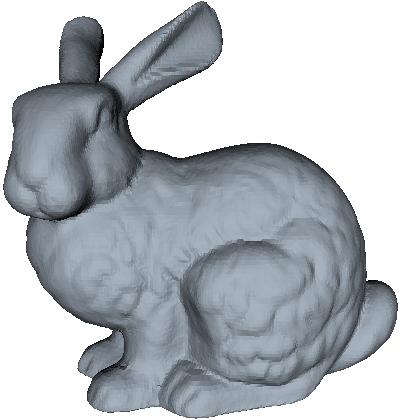
\includegraphics[width=2.5in]{images/ch2/bunny}
                \caption{original}
                \label{fig:bunnyOrigAA}
        \end{subfigure}
        \begin{subfigure}[b]{2.5in}
                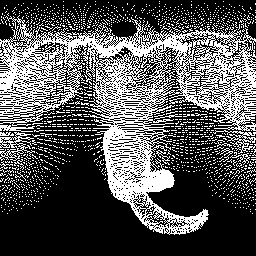
\includegraphics[width=2.5in]{images/ch2/spherical2DMap}
                \caption{transform}
                \label{fig:bunnySPTed}
        \end{subfigure}%
        \caption{The Spherical Map Transform.}
       \label{fig:smtExample}
\end{figure}


Equation \ref{eqn:invLPVVF} is a vector valued function with three separate functions for the x, y and z axis components. These functions are found in equation \ref{eqn:invLPFuncs}. The x-axis function $Ray_x(x,y,r)$ is used together with the $Ray_y(x,y,r)$ and $Ray_z(x,y,r)$ functions to form a spherical transform. The reduction in dimension is achieved by summing the components which share x and y coordinates but have different $r$ (radius) values. In these equations the 3D volume $Vol$ has a width, height and depth of $N$ whilst the output image $Im$ has a width and height of $M$. \\


\begin{equation} \label{eqn:invLPFuncs}
\begin{split}
Ray_x(x,y,r) & = r \times cos\left(\frac{360x}{M}\right)sin\left(\frac{180y}{M}\right)  + \frac{N}{2} \\
Ray_y(x,y,r) & = r \times cos\left(\frac{180y}{M}\right) + \frac{N}{2} \\
Ray_z(x,y,r) & = r \times sin\left(\frac{360x}{M}\right)sin\left(\frac{180y}{M}\right) + \frac{N}{2}
\end{split}
\end{equation}

\begin{equation} \label{eqn:invLPVVF}
Ray(x,y,r) = [Ray_x(x,y,r), Ray_y(x,y,r), Ray_z(x,y,r)]^T
\end{equation}

\begin{equation} \label{eqn:smtUpdate}
Im_{x,y} = \sum_{r=1}^{(2^{-1}N)^{1.5}}{Vol(Ray(x,y,r))} 
\end{equation}

In the Log-Spherical transform described in section \ref{Sec:RoteZoomingSection} re-arranges the rotation and scale transforms along two axis, the third axis retains information and increases the accuracy of the solution. By reducing the other axis from size $N$ to the average value (size 1) information is lost, however computational complexity is reduced by an entire dimension. This is a complexity/performance trade off. Computational complexity may be afforded given input data contains relatively little noise. The output image maps 3D y-axis rotation to 2D x-axis translation is the output image. \\


This process essentially sums up the values along a given ray defined by scaling spherical coordinates and adding up the values intersecting the ray. The resulting image, maps 3D y-axis rotation to 2D x-axis translation. Once two 3D frame volumes $V_a$ and $V_b$ are transformed into their corresponding spherical-map domain $SM_a$ and $SM_b$ respectively, the two may be phase correlated  in order to measure the x-axis translation separating them. This x-axis translation may then be mapped directly to the rotational angle separating the two input 3D camera frames.The relationship may be computed as $\frac{360x}{M}$ where $x$ is the a-axis translation and $M$ is the width and height of the spherical map domain image. \\


\subsubsection{Projection-map transform}
\label{sec:PMTramsform}

The projection map transform is similar in spirit to an orthogonal projection of the volume along a particular axis. Instead of simply projecting the closest point as in projection for visualization purposes, the sum of values computed along the ray is used for representation. The projection map transform is described here in terms of an output projection map image $Im$ and an input 3D volume frame $Vol$, which may be input from a sensor or software system which is able to generate 3D frames of the environment. Each pixel in $Im$ has its value defined mathematically as the summation of values along a particular axis given the x,y coordinates. The Projection-map x-axis transform and the Projection-map z-axis transform are defined in equations \ref{eqn:xPMT} and \ref{eqn:zPMT} respectively. \\

WARNING: add in a picture here

\begin{equation} \label{eqn:xPMT}
Im(z,y) = \sum_{x=0}^{N}{Vol(x,y,z)}
\end{equation}

\begin{equation} \label{eqn:zPMT}
Im(x,y) = \sum_{z=0}^{N}{Vol(x,y,z)}
\end{equation}

In these equations the Projection map transform along the x-axis is computed via summing up values along the x-axis in the input 3D frame,. In this was, any 3D z-axis translation in $Vol$ maps to 2D x-axis translation in the output image $Im$. Additionally any y-axis translation in the input 3D frame $Vol$ is mapped to a corresponding y-axis translation in the output 2D Projection map domain $Im$. If both the width and height of the output image $Im$ is equal to the width, height and depth of the input 3D frame then the relationship is a $1:1$ mapping between 3D z-axis translation and 2D x-axis translation as well as 3D y-axis translation to 2D y-axis translation. \\

The corresponding z-axis Projection map transform sums up values along the z-axis. Here, 3D y-axis translations within the original 3D frame also produce 2D y-axis translations in the output Projection map domain. However, all x-axis translations occurring within the 3D frame domain are mapped to 2D x-axis translations in the output Projection map domain image $Im$. \\

Given both of these Projection map transforms, the 3D translation separating two 3D frames may be registered with respect to 3D translation. This 3D translation also has an inverse relationship to the camera location separation between the two frames. Both 3D frames are transformed into the z-axis Projection map domain. By phase correlating these domains, both the x and y axis translation may be retrieved which map directly to the 3D translation x and y coodinates separating the input frames. The 3D z-axis translation may be computed by transforming both frames into the x-axis Projection map domain. Once the two Projection map domains are phase correlated, the x-axis translation separating the domains can be mapped directly to the corresponding z-axis translation separating the two input 3D frames. In total, using $2 \times$ Projection map transforms and $1 \times$ 2D phase correlation method, the 3D translation parameters separating two 3D frames may be computed. \\

\subsubsection{Performance Analysis}

In order to assess the efficiency gain between the Fast Fourier Volume Registration method over the original FVR method, the computational complexity of the FVR is assessed. The computational complexity is dependent on two factors: the size of the input depth map $W \times H$ and the width/height/depth of the 3D volumes used in the volume registration procedure. Since the computational complexity is fixed no matter the input data (depending only on the sizes specified by the user), this method is considered a closed form solution. \\

The FVR method makes use of several sub-procedures including: projection of the depth frame to a 3D volume frame, 2 $\times$ Hanning window filters, 2 $\times$ 3D FFTs, 2 $\times$ element-wise Log filters, 2 $\times$ Log-spherical transforms, 2 $\times$ 3D phase correlation processes, 1 $\times$ linear transformation and 1 $\times$ peak search. The number of operations required by each of these methods are listed in table \ref{table:complexities} \\

%translation
\begin{table}[ht]
\centering
\scalebox{0.75}{
\begin{tabular}{cc}
\hline
\textbf{Procedure} & \textbf{Complexity}\\ \hline
Hanning window & 26 (GPGPU)\\
3D FFT & $N^3\log{N^3}$ (GPGPU)\\
Log & 3 (GPGPU) \\
Log-Spherical & 58 (GPGPU)\\
Multiplying Spectra & 15 (GPGPU)\\
Geometric Transform & 30 (GPGPU)\\
Peak Search & $2N^3$\\
\\
\end{tabular}}
\\
\caption{Complexities for given Procedures}
\label{table:complexities}
\end{table}[ht]

The Hanning windowing function requires 26 operations. The 3D FFT has complexity of $3N^3\log{N}$, the log and log-spherical transform functions require 3 and 58 operations per voxel respectively. Multiplying two frequency spectra together and transforming a volume requires 15 and 30 operations per voxel respectively. Finding the peak value requires $2N^3$ operations. The complexity in terms of number of operations for the phase correlation process is given in Eq. \ref{eqn:PCFULLPERFORMANCE} This process requires 2 $\times$ 3D FFTs, 1 $\times$ frequency spectra multiplication, and 1 $\times$ peak finding operation. 
\begin{equation} \label{eqn:PCFULLPERFORMANCE}
6N^3\log{N} + 2N^3 + 15
\end{equation}
The total complexity can then be found by taking into account the projection and re-sampling totals as well as the total for $VolumeRegister{\theta \varphi t_x t_y t_z}(V_1, V_2)$. Tallying the number of operations for each process and multiplying them by number of times the process is performed gives us the number of operations as a function of $W$, $H$ and $N$ in Eq. \ref{eqn:FULLPERFORMANCE}.
\begin{equation} \label{eqn:FULLPERFORMANCE}
6N^3 + 28WH + 18(N^3\log{N}) + 230
\end{equation}

To compare performance of the generic volume registration method with the speed up, we use the complexity defined in equation \ref{eqn:FULLPERFORMANCE}. Here, we ignore the cost of projecting the depth map. The 3D DFT has complexity $3N^3log(N)$. This is the first step (see figure \ref{fig:PIPELINE3}), the next is the spherical-map transform which is complexity $45N^3$. If processed on the GPU the performance becomes 45 operations per voxel assuming that one voxel is assigned to one unit of processing. A 3D transform is 30 operations per voxel, 2D phase correlation requires 15 operations to multiply the frequency spectra and $2N^2log(N)$ operations to do the 2D FFT. Finally a projection map transform requires 1 operation per voxel. \\

In total, the proposed method requires $2 \times$ 3D FFTs, $2 \times$ spherical-map transforms, $1 \times$ 3D geometrical transformation, $3 \times$ 2D phase correlations and $4 \times$ projection map transforms. The total complexity is added up for all of these functions and given in equation \ref{eqn:FULLPERF2}. \\

\begin{equation} \label{eqn:FULLPERF2}
6log(N)\times (N^3 + N^2) + 169
\end{equation}

Figure \ref{fig:perfComp} provides a visualization of the performance improvement which the proposed method achieves over the original Fourier volume registration approach. It is clear that the proposed method is around 3 times faster
than the original Fourier based volume registration approach. This is due to the reduction in the amount of data to process afforded by the novel spherical-map transform and orthogonal projection methods.

\begin{figure}[!htb]
\centering
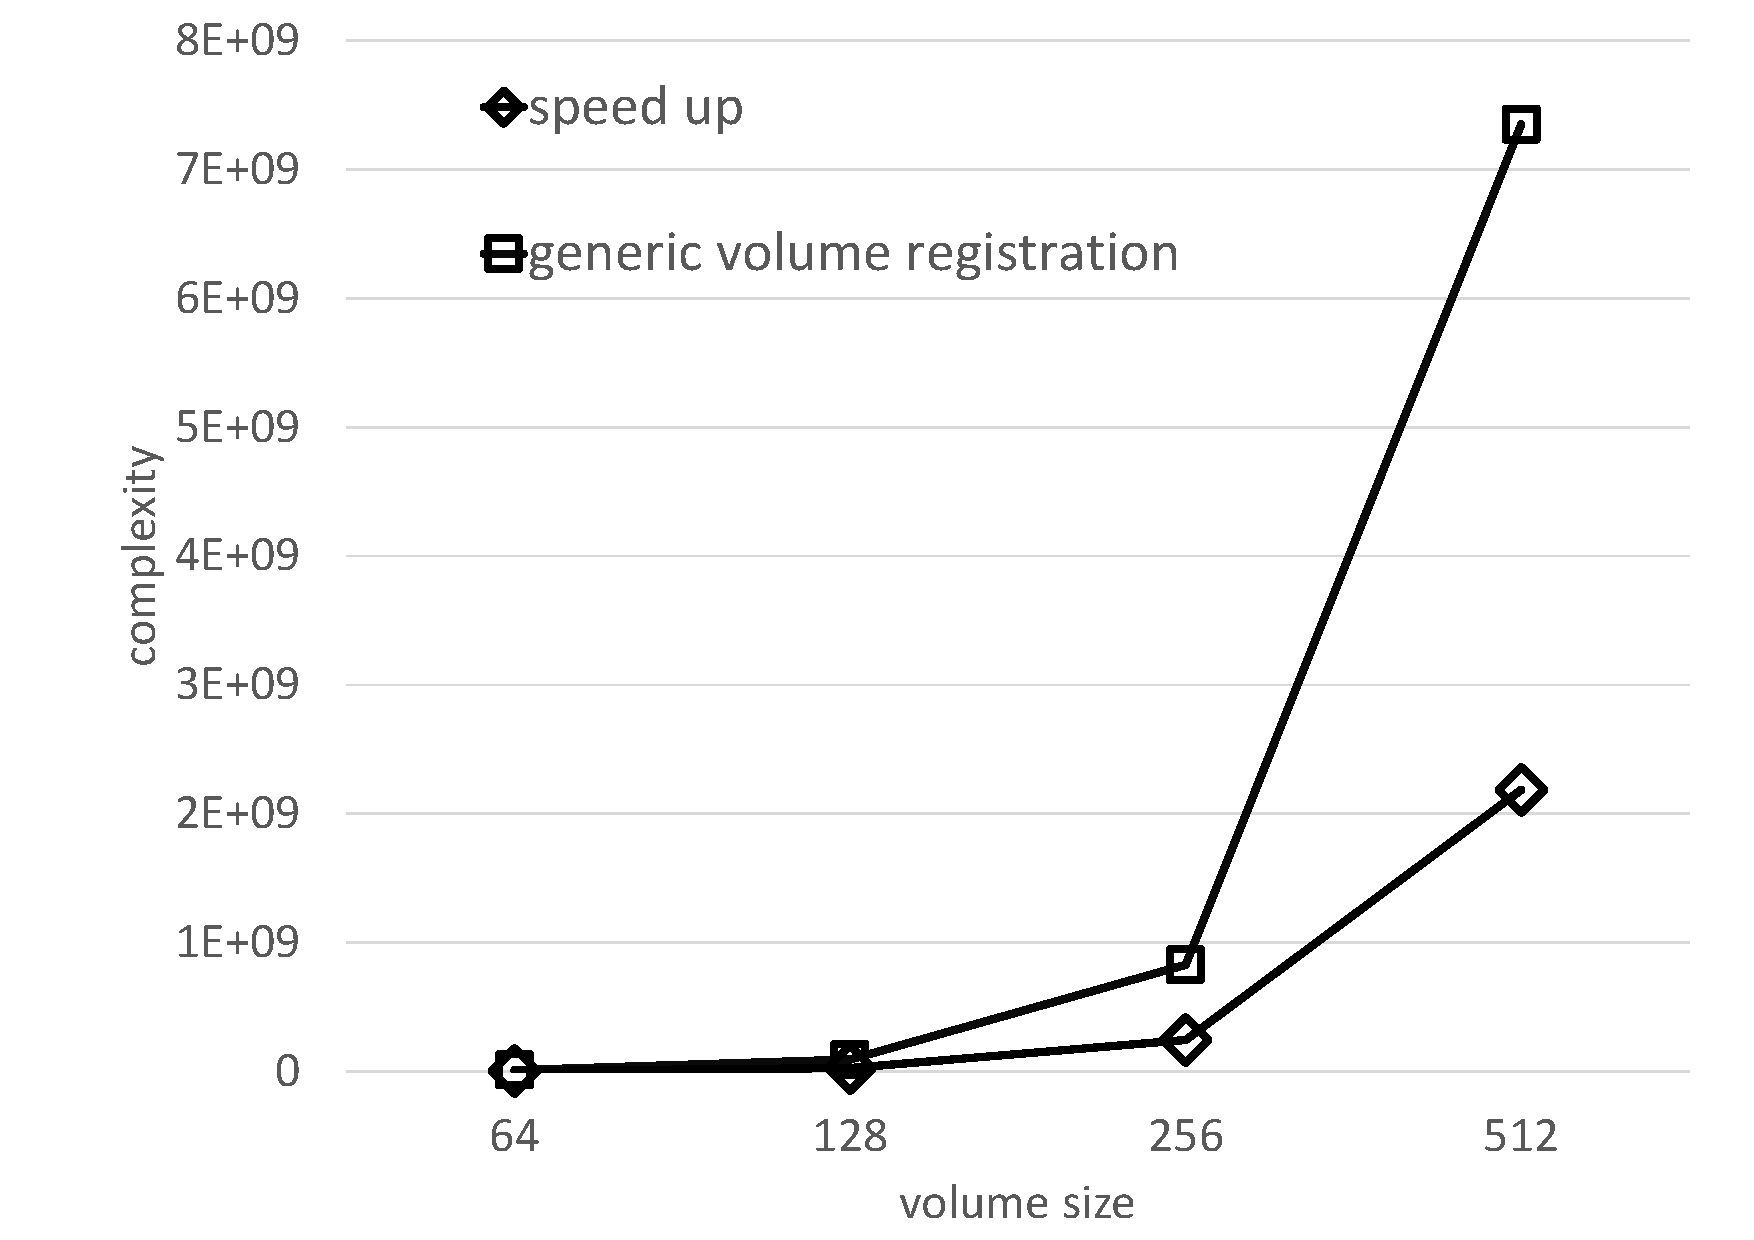
\includegraphics[width=4.0in]{images/ch2/perfcomp}
\caption{Comparison of performance between volume registration and the proposed speed up for different volume sizes.}
\label{fig:perfComp}
\end{figure}

\section{Full 3D Rotation Recovery and Reconstruction}

This section explains how the FVR algorithm may be extended to recover full 3D camera pose rotation in addition to translation and scale differences between a pair of captured 3D frames. We propose a novel method which uses Principal Components Analysis (PCA) as a pre-processing step to achieve full 3D rotation estimation. This method is named FVR-3D. The FVR method, the FFVR method and the FVR-3D method all have unique advantages and disadvantages. FVR is designed to be an accurate and efficient method of estimating camera pose and location on wider baselines whilst remaining robust to the effects of noise. It is robust to 3D rotations (not just y-axis rotation) but cannot register them, if 3D rotation recovery is required, the FVR-3D method discussed in this section provides an efficient solution, but is less robust to noise and wider baselines. The FFVR method may also be used, it works similarly to the FVR method but is computationally more efficient at the expense of accuracy and noise robustness. FFVR also cannot handle wide baselines well, but is up to 4 times more efficient than the FVR for realistic volume sizes. \\

To integrate 3D rotation into the standard FVR method, a single axis relating the two 3D models must be known. If such an axis is known prior to executing the FVR method, both 3D frames may be aligned vertically (along the y-axis) with respect to the found axis. Once aligned, the FVR method may be used to register both frames relative to the final y-axis rotational separation which can be used to recover rotation and scale factors so translation may also be recovered. \\

Several techniques were explored to compute this commonly rotated axis. These include computing the average normal value, the axis defined as the vector between the furthest two points as well as other techniques based on feature matching. The use of PCA was also tested. Based on empirically driven factors, PCA was chosen to compute the common axis for use in the FVR-3D method. PCA may be used to compute the full rotation separating two 3D frames but this typically fails when noise or non-overlapping parts of the frames are present. To be more robust to noise and non-overlapping features within the frame, only the primary axis is used to align both frames with their primary axes pointing directly up. This alignment is more robust because the primary axis has a stronger presence within the data. Once the y-axis rotation is solved, the full 3D rotation factors may be computed via the FVR method. \\

Experiments evaluating FVR-3D in section \ref{Sec:FVRSOTA} show it outperforms other popular methods used for 3D camera pose estimation in terms of accuracy on a wide range of scene types. Additional experiments prove its robustness in the face of noise when registering camera pose. \\

\subsubsection{Computing a Principal Axis}

Using PCA to compute the principal axis used in FVR-3D is discussed in this section. Both 3D frames have their axis computed separately before they are used to align both frames to a common axis. To compute the common axis using PCA, both the eigen-values and eigen-vectors of the covariance matrix of the 3D frames must be computed. The eigen-vector with the largest corresponding eigen-value is set as the primary axis. The procedure works as follows. \\

Given a 3D point cloud $A$ of $N$ points, which may be generated via monocular methods, stereo disparity estimation or active sensor (Kinect, Asus XTion Pro-LIVE), the co-variance of the points between two of the dimensions ($x$ and $y$) is computed as the summation of each $x$ component subtracted by the mean $x$ value multiplied by the $y$ component subtracted by the mean $y$ component value (see equation \ref{eqn:Covariance3DSignal}, $A_{x_{mean}}$ and $A_{y_{mean}}$ refer to the mean values of these x and y dimensions of $A$). \\

\begin{equation} \label{eqn:Covariance3DSignal}
Cov(A_x,A_y) = \sum_{i=0}^{N}(A_{x_i} - A_{x_{mean}})(A_{y_i} - A_{y_{mean}})
\end{equation}

Using the formula for covariance the covariance matrix may be computed for an $N$ dimensional signal. In the case of 3D construction, this matrix is a $3 \times 3$ covariance matrix where each column/row index represents a covariance relationship. This covariance matrix is shown in equation \ref{eqn:CovarMatrix}. This matrix describes how each coordinate axis changes with respect to each other coordinate. The eigen-vectors of this matrix constitute the principal components of the 3D point cloud frame. \\

\begin{equation} \label{eqn:CovarMatrix}
\left[
\begin{array}{ccc}
Cov(A_x, B_x) & Cov(A_x, A_y) & Cov(A_x, A_z) \\
Cov(A_y, B_x) & Cov(A_y, A_y) & Cov(A_y, A_z) \\
Cov(A_z, B_x) & Cov(A_z, A_y) & Cov(A_z, A_z) \\
\end{array}
\right]
\end{equation}

The three eigen-vectors of the covariance matrix describe the primary axis of the 3D frame $A$ and the three corresponding eigen-values describe the dominance of these vectors. The eigen-vector/axis with the largest corresponding eigen-value is the principal component in PCA and is used as the aligning axis in the FVR-3D method. This principal axis is used to align data to a common axis defined as the vertical y-axis. For simplicity, the principal axis of a 3D frame $A$ is written as $A_{pa}$. During the PCA process, the centroid of the point cloud is also computed. This is simply the average point location within the input point cloud. For simplicity in later discussions, the centroid of a 3D frame $A$ is written as $A_{mean_{location}}$. A visualization of the principal axis and centroid are shown in Figure \ref{fig:FVR3D111}. Here two input frames (Figures \ref{fig:fvr3DINA} and \ref{fig:fvr3DINB}) are corrected such that their mean is translated to the centre of the volume and their principal axis is aligned with the vertical axis (Figures \ref{fig:fvr3DAAlign} and \ref{fig:fvr3DBAlign}). \\

\begin{figure}[!htb] 
        \centering
        \begin{subfigure}[b]{3.0in}
               \centering
                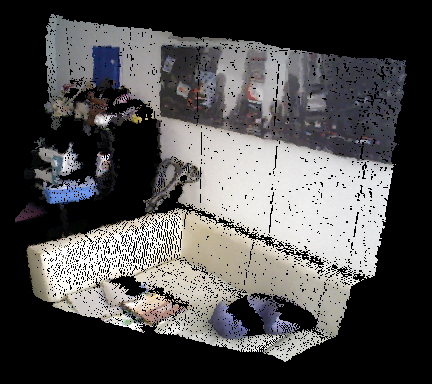
\includegraphics[width=2.0in]{images/methodology/FVR/fvr3d/frameA}
                \caption{Frame A}
                \label{fig:fvr3DINA}
        \end{subfigure}%
        \begin{subfigure}[b]{3.0in}
        		\centering
                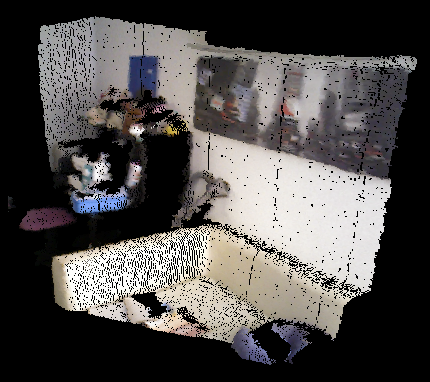
\includegraphics[width=2.0in]{images/methodology/FVR/fvr3d/frameB}
                \caption{Frame B}
                \label{fig:fvr3DINB}
        \end{subfigure}
        
         \begin{subfigure}[b]{3.0in}
         		       \centering
                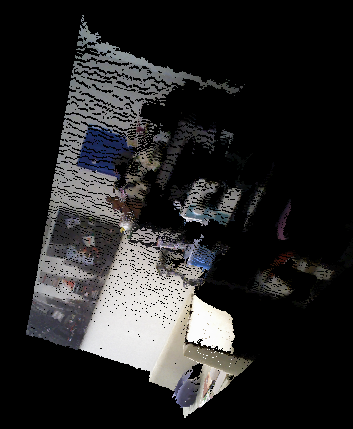
\includegraphics[width=2.0in]{images/methodology/FVR/fvr3d/PCAFrameA}
                \caption{Frame A, PCA aligned}
                \label{fig:fvr3DAAlign}
        \end{subfigure}%
         \begin{subfigure}[b]{3.0in}
                \centering
                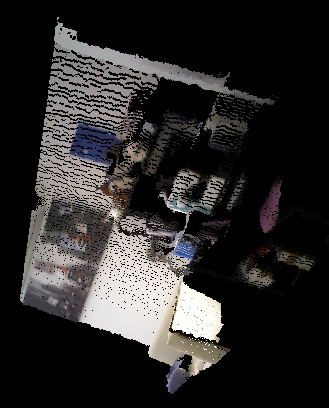
\includegraphics[width=2.0in]{images/methodology/FVR/fvr3d/PCAFrameB}
				\caption{Frame B, PCA aligned}
                \label{fig:fvr3DBAlign}
        \end{subfigure}
        

       \caption{Early stages of FVR-3D}
       \label{fig:FVR3D111}
\end{figure}



\subsubsection{Alignment Pre-Process}

Using the PCA method, for each input 3D frame $V$, the computed principal axis $V_{pa}$ and the centroid $V_{mean_location}$ are used to align the input 3D frame using $V_{pa}$ as the new vertical axis. To this end, a transformation matrix is formed and used to rotate the volume so the principal axis $V_{pa}$ points up. This is useful because if a 3D frame pair are both rotated with respect to their principal axis, and both frames share enough overlap, then only 3D y-axis rotation, 3D translation (and possibly 3D scale) separate the two frames. As discussed in section \ref{Sec:AFVRApproach}, these parameters may be recovered using the FVR method. The matrix used to normalize the 3D frames in terms of their principal axis is discussed here. \\

If $V_{pa}$ (the vector pointing along the principal axis of $V$) is to be set as the new y-axis for the volume, then the other axes must also be computed (x-axis and z-axis). The z-axis, named the forward ($Fwd$) axis, is computed based on the cross product between the then x-axis and the principal axis $V_{pa}$ (taken as the y-axis) which gives a psuedo z-axis. The cross product between the principal axis and this pseudo z-axis gives an accurate x-axis. Lastly the cross product between this x-axis and the y-axis (the principal axis) gives the corresponding z-axis in the form of the variable $Fwd$. This is shown in equation \ref{eqn:fwdVector}. \\


\begin{equation} \label{eqn:fwdVector}
Fwd = \left(\left[
\begin{array}{c}
V_{pa_{x}}\\
V_{pa_{y}}\\
V_{pa_{z}}\\
\end{array}
\right] \times \left(\left[
\begin{array}{c}
1\\
0\\
0\\
\end{array}
\right] \times \left[
\begin{array}{c}
V_{pa_{x}}\\
V_{pa_{y}}\\
V_{pa_{z}}\\
\end{array}
\right]\right)\right) \times \left[
\begin{array}{c}
V_{pa_{x}}\\
V_{pa_{y}}\\
V_{pa_{z}}\\
\end{array}
\right]
\end{equation}

The final axis completing the new space is the x-axis defined at the cross product between the principal axis (the new y-axis) and the z-axis (the $Fwd$ vector) and is named $Rgt$ (standing for right facing axis). Equation \ref{eqn:rgtVector} shows this calculation. The new space is now defined by x-axis $Rgt$, y-axis $V_{pa}$ and z-axis $Fwd$. A rotation matrix transforming original space to the new space defined by these axes may be computed using the $Rgt$, $V_{pa}$ and $Fwd$ axes as the column vectors of the rotation matrix. The inverse, that is the transformation from the new space to the original space may be computed using the transpose of the rotation matrix. The rotation of the point cloud from the new space defined by the principal axis to the original space is useful as it aligns the principal axis to the y-axis leaving only 3D y-axis rotation, 3D translation and possibly scale to be registered. \\ 


\begin{equation} \label{eqn:rgtVector}
Rgt = \left[
\begin{array}{c}
V_{pa_{x}}\\
V_{pa_{y}}\\
V_{pa_{z}}\\
\end{array}
\right] \times \left[
\begin{array}{c}
Fwd_x\\
Fwd_y\\
Fwd_z\\
\end{array}
\right]
\end{equation}

The input 3D frame $V$ may be aligned by its principal axis as the new y-axis by first transforming the centroid to the origin. Next the 3D frame may be rotated from the new space to the default identity space. This sets $Rgt$ as the new x-axis, $V_{pa}$ as the new y-axis and $Fwd$ as the new z-axis. The rotation matrix may be computed as the row vectors of these axes. Finally, after rotation the 3D frame $V$ may be transformed back to the centroid. This aligns the 3D frame so that $V_{pa}$ points towards the y-axis. The compounded transformation to perform this alignment is fully defined in equation \ref{eqn:CorrectUpMat}. \\

\begin{equation} \label{eqn:CorrectUpMat}
CorrectMat(V) = \left[
\begin{array}{cccc}
1 & 0 & 0 & V_{mean_x} \\
0 & 1 & 0 & V_{mean_y} \\
0 & 0 & 1 & V_{mean_z} \\
0 & 0 & 0 & 1 \\
\end{array}
\right] \left[
\begin{array}{cccc}
Rgt_x & Rgt_y & Rgt_z & 0 \\
V_{pa_x} & V_{pa_y} & V_{pa_z} & 0 \\
Fwd_x & Fwd_y & Fwd_z & 0 \\
0 & 0 & 0 & 1 \\
\end{array}
\right] \left[
\begin{array}{cccc}
1 & 0 & 0 & -V_{mean_x} \\
0 & 1 & 0 & -V_{mean_y} \\
0 & 0 & 1 & -V_{mean_z} \\
0 & 0 & 0 & 1 \\
\end{array}
\right]
\end{equation}

\subsubsection{3D Rotation Registration}

To recover a matrix for full 3D rotation separating two input 3D frames $A$ and $B$ which have been taken from two different locations (translation separation) with two different poses (3D rotational separation) and possibly projected differently (scale separation), the first step is to align both frames by their principal axis. The alignment matrix for $A$ can be computed as $C_A = CorrectMat(A)$ and the alignment matrix for $B$ may be computed as $C_B = CorrectMat(B)$. Transforming both $A$ and $B$ by their alignment matrix gives two volumes $A_{aligned} = Transform(A, C_A)$ and $B_{aligned} = Transform(B, C_B)$ which are now only separated by 3D y-axis rotation, 3D translation and 3D scaling factors. As discussed in sections \ref{Sec:VolumeRegistrationSection} and \ref{Sec:AFVRApproach} these factors may be computed and a registration matrix aligning $A_{aligned}$ and $B_{aligned}$ generated. This matrix is computed as $R_{y}ST = FVR(A_{aligned},B_{aligned})$. Using this registration matrix and the alignment matrices $C_{A}$ and $C_{B}$, the full 3D registration matrix $R_{x,y,z}ST$, which transforms $A$ to $B$, may be computed. Matrix $R_{x,y,z}ST$ aligns $A$, registers it using $R_{y}ST$ (which aligns it with $B_{aligned}$) then inverse transforms it by $C_{B}$ which un-aligns it according to alignment matrix $C_B$. This can be followed as in equation \ref{eqn:FullRSTTransform}. \\


Figure \ref{fig:FVR3D222} (along with Figure \ref{fig:FVR3D111}) shows the output at different stages of the FVR-3D technique. Once two input frames (Figures \ref{fig:fvr3DINA} and \ref{fig:fvr3DINB}) are aligned via PCA (Figures \ref{fig:fvr3DAAlign} and \ref{fig:fvr3DBAlign}), they must be registered using the FVR method. This is shown in Figure \ref{fig:fvr3DFVRPCAAB}, as without any further registration, the reconstruction would not be correct (see Figure \ref{fig:fvr3DPCAAB}). By reversing Frame B's PCA alignment stage on the frame in Figure \ref{fig:fvr3DFVRPCAAB} the full FVR-3D registration output is revealed (Figure \ref{fig:fvr3DFVRPCAAB}). This registration is very accurate in comparison to zero registration being performed prior to integration, which is shown in Figure \ref{fig:fvr3DPCAAB}. \\
 

\begin{equation} \label{eqn:FullRSTTransform}
R_{x,y,z}ST Matrix = C_{B}^{-1} \times R_{y}ST \times C_A
\end{equation}

FVR-3D is a capable registration method which extends Fourier registration to take into account full 3D rotation. The complexity of the technique adds a single layer of complexity over the FVR method. The additional computational complexity ($N^3$), which is primarily made up of computing the covariance matrix, is minimal compared to the rest of the FVR technique. \\


\begin{figure}[!htb] 
        \centering
        
		\begin{subfigure}[b]{3.0in}
				       \centering
                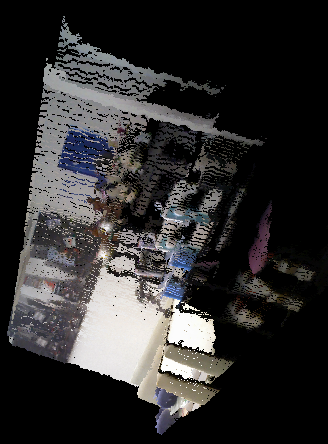
\includegraphics[width=2.0in]{images/methodology/FVR/fvr3d/PCAFrameAB}
                \caption{\ref{fig:fvr3DAAlign} and \ref{fig:fvr3DBAlign} integrated}
                \label{fig:fvr3DPCAAB}
        \end{subfigure}%
        \begin{subfigure}[b]{3.0in}
               \centering
                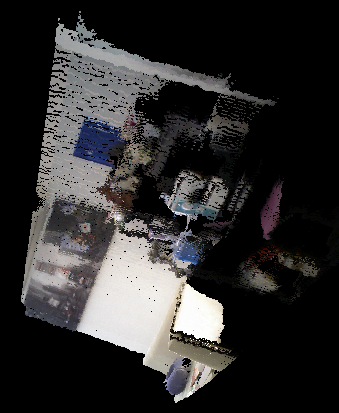
\includegraphics[width=2.0in]{images/methodology/FVR/fvr3d/FVRPCAFrameAB}
                \caption{\ref{fig:fvr3DAAlign} registered with \ref{fig:fvr3DBAlign} using FVR}
                \label{fig:fvr3DFVRPCAAB}
        \end{subfigure}        
        
        \begin{subfigure}[b]{3.0in}
               \centering
                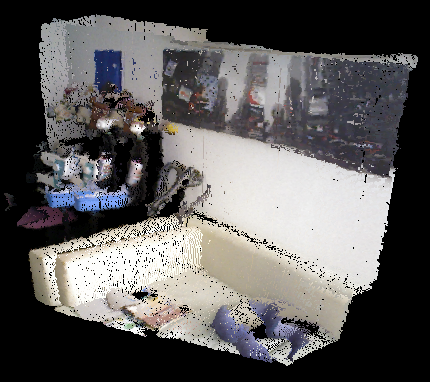
\includegraphics[width=2.0in]{images/methodology/FVR/fvr3d/noRegistration}
                \caption{\ref{fig:fvr3DINA} and \ref{fig:fvr3DINB} integrated}
                \label{fig:fvr3DPCAAB}
        \end{subfigure}%
        \begin{subfigure}[b]{3.0in}
               \centering
                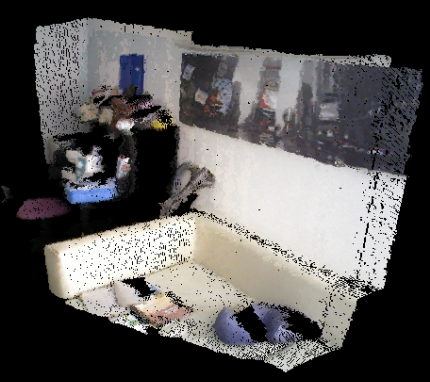
\includegraphics[width=2.0in]{images/methodology/FVR/fvr3d/FVR3DReg}
                \caption{\ref{fig:fvr3DFVRPCAAB} un-aligned (full FVR-3D registration)}
                \label{fig:fvr3DFVRPCAAB}
        \end{subfigure}        
        
       \caption{Final stages of FVR-3D}
       \label{fig:FVR3D222}
\end{figure}



\subsubsection{Algorithm and Pipeline}

\label{METHOD_SECLL}

The proposed SLAM/3D reconstruction routine for the FVR-3D is almost identical to the routine for the FVR method in Listing \ref{algorithm:PCSLAMNo1}. First, the 3D frame $f_1$ is read in and projected to construct a point cloud $PointCloud$. $PointCloud$ is then integrated using volumetric integration into the global reconstruction. Matrix $M$ is initialized to the identity matrix to accumulate the registration matrices so future frames may be efficiently integrated. $Camera_{location}$ and $Camera_{pose}$ accumulate camera location and 3D rotational pose, respectively, and are combined and listed in $Cameras$ on a per frame basis. These variables may be omitted in the case of 3D reconstruction, or output in the case of 3D SLAM. Next, a loop is used for each new frame input into the system. In this loop, 3D frame $f_2$ is read in. Both $f_2$ and $f_1$ are projected and voxelized into $V_1$ and $V_2$, respectively. \\

\begin{figure}
\begin{lstlisting}[language=c++,caption=Phase Correlation Based SLAM Algorithm,label=algorithm:FVR3DSLAM,mathescape,basicstyle=\ttfamily]
$f_1$ = ReadFrame();
$PointCloud$ = project($f_1$);
$GlobalReconstruction$.integrate($PointCloud$)
$M$ = IdentityMatrix();
$Camera_{location}$ = $[0, 0, 0]^T$;
$Camera_{pose}$ = $[[1, 0, 0]^T,[0, 1, 0]^T,[0, 0, 1]^T]$;
$Cameras$ = $\left[\left[Camera_{location}, Camera_{pose}\right] \right]$;
while(more frames){
	$f_2$ = ReadFrame();
	$points_1$ = project($f_2$);
	$points_2$ = project($f_1$);
	$V_1$ = Voxelize($points_1$);
	$V_2$ = Voxelize($points_2$);
	$R_{x,y,z}ST$ = $FVR-3D_{\theta \varphi t_x t_y t_z}(V_1, V_2)$;
	$Temp$ = $R_{x,y,z}ST$;
	$M = M \times Temp$;
	$points_1$ = Transform($points_1$, $M$);
	$GlobalReconstruction$.integrate($points_1$);
	$Camera_{location}$ = $Temp^{-1} \times Camera_{location}$;
	$Camera_{pose}$ = $Temp^{-1} \times (Camera_{pose} + Camera_{location})$;
	$Camera_{pose}$ = $\frac{Camera_{pose} - Camera_{location}}{Camera_{pose} - Camera_{location}}$;
	$Cameras.add(\left[Camera_{location}, Camera_{pose}\right])$;
	$f_1$ = $f_2$;
}
\end{lstlisting}
\end{figure}

Next, the FVR-3D method is used in place of the FVR method to compute the full six (plus 1 for scale) degrees of freedom required for 3D SLAM or 3D reconstruction. A temporary variable $Temp$ is used to hold this rigid transformation matrix. $M$ is then updated to take into account the previous registration transforms plus the current one. Using the updated transformation matrix, $M$ is applied to $points_1$ to register it with the current global reconstruction, then integrated with the final reconstruction. Next, $Camera_{location}$ and $Camera_{pose}$ are updated and the new camera pose and location values are added to the $Cameras list$. \\



Figure \ref{fig:PIPELINE8} shows a pipe-line for the FVR-3D technique. Here, two 3D frames are input as $Volume_1$ and $Volume_2$. The second frame may be taken after the camera has changed location and pose. The two frames may also be taken by different cameras with differing projection procedures projecting depth map values into frames. First the alignment matrices $C_a$ and $C_b$ based on the principal axis are computed by the PCA algorithm. These matrices are then used to align $Volume_1$ and $Volume_2$ to a common axis. Only then can the proposed FVR method be used to register the final axis of rotation along with scale and translation changes. Finally a full registration matrix may be formed by the alignments matrices and the output registration matrix via the FVR procedure. \\

\begin{figure}[!htb]
\centering
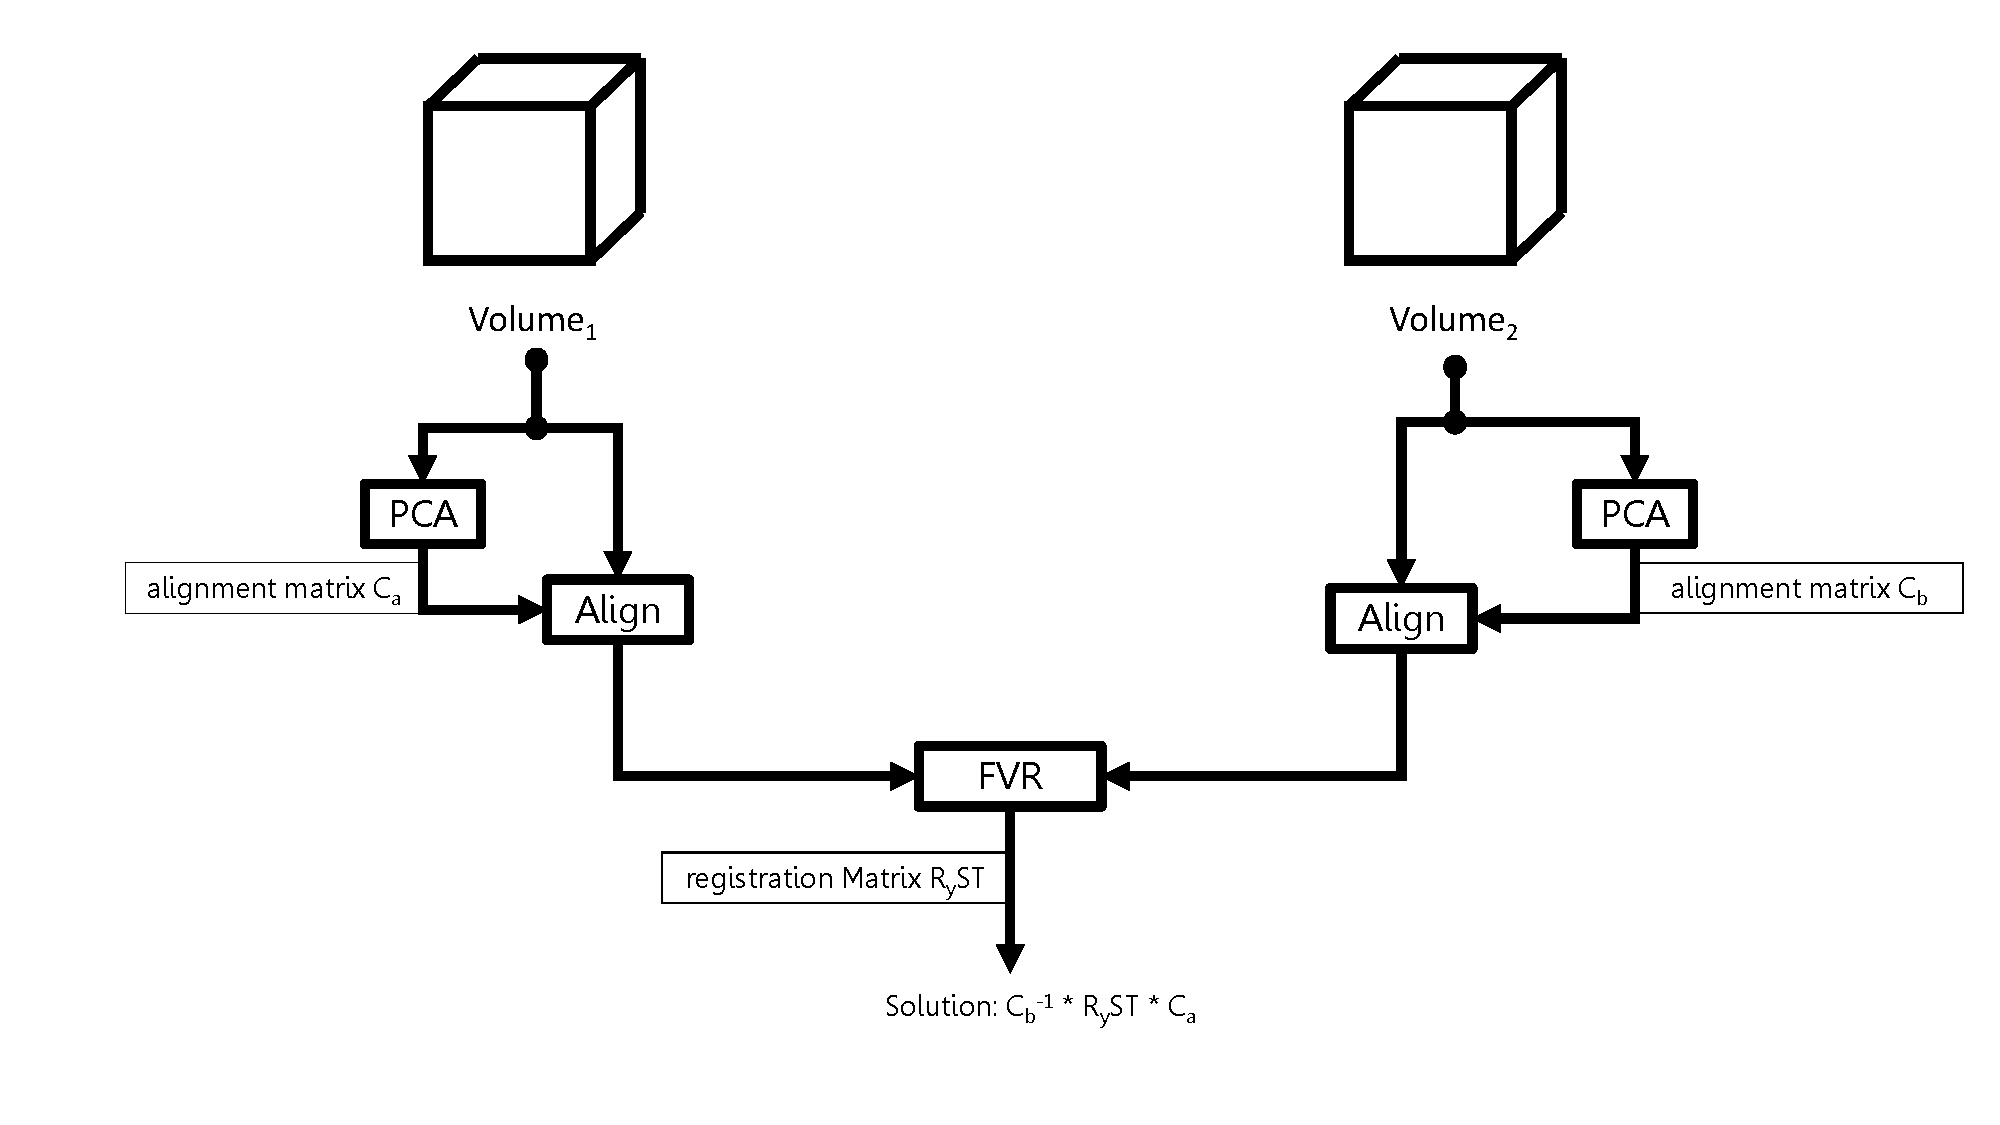
\includegraphics[width=6.0in]{images/methodology/FVR/pipeline8}
\caption{System Diagram for Registration Process}
\label{fig:PIPELINE8}
\end{figure}


\subsubsection{Limitations}

Experiments (sections \ref{Sec:FVRSOTA} and \ref{Sec:CamTransTrackExp}) show that the FVR-3D algorithm is a capable 3D reconstruction method in terms of accuracy, however, it is less robust to noise and wide-baselines than the FVR method. This is due to PCA being much more affected by noise than the FVR method on its own. Therefore, whilst the FVR method is limited to y-axis rotational registration, it is more robust under noisy conditions. To solve this noise issue associated with FVR-3D, the plain FVR method is also used whenever FVR-3D is used and the best registration is chosen on a per frame basis. Despite the reduced accuracy at wide baselines or when more noise is present, the FVR-3D method outperforms several state-of-the-art algorithms used in registering 3D frames produced by different sensor types, including: stereo and active camera set-ups. \\






\section{Conclusion} % Fourier Volume Registration
\begin{savequote}[8cm]
  ``I have not failed. I've just found 10,000 ways that won't work.''
  \qauthor{Thomas Edison}
\end{savequote}
\makeatletter
\chapter{Data Representation and Compression}

\section{3D Reconstruction Data Representation}
\label{sec:3DDataRepresentations}
In this section a novel 3D frame data representation and compression method is described. It was designed to help reduce data size whilst facilitating data processing. This novel representation is named Plane-Tree and is a modification of the basic Octree 3D data representation method. \\

The Shade-Tree is designed primarily to compress 3D data. It is based on the Octree but was inspired by the Shade-Tree and Interpolated Leaf Quad-Tree representations \cite{Gonzalez07ShadeTree, Lincoln13Interpolating} which are used for image compression. These techniques make use of Quad-Tree decomposition and have been shown to outperform several transform based methods of compression. 

\subsection{Octree Overview}

In this section Octree decomposition is explained. This strategy forms a cubic shaped space around some 3D data. In the case of 3D reconstruction, it may be the 3D frame input from an active sensor, stereo method or monocular depth estimation procedure. A geometric representation is then computed for the data contained within the cubic space. This representation may be as simplistic as recording the cube's center or using the cube to represent the space, or may be complex, employing splines and curvature representation techniques to represent the space. \\

Whatever the representation, a measurement system must be used to decide whether the computed geometric representation fits the data within the space adequately. If the geometric representation is accurate enough for application purposes, then it may be used in place of the data. This representation is typically designed such that the amount of data required for representation of a space is less than the amount which would be used otherwise. Alternatively, the representation may make use of known correlations which may be more easily compressed compared with the initial representation. \\


\begin{figure}[!htb]
\centering
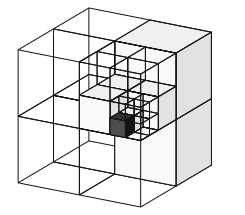
\includegraphics[width=8cm]{images/methodology/pt/octreeVis}
\caption{Visualization of cubic space being split \cite{Hornung13Octomap}.}
\label{fig:SpaceVis}
\end{figure}

If, by the error generated via the measurement system, it is decided the representation is not suitable, the cubic space is broken down into 8 sub-cubes and the process is repeated. For an example of the space broken down into sub-cubes see figure \ref{fig:SpaceVis}. \\

At each level of decomposition, the data representation achieves finer detail, but more nodes must be stored which means less compression. This is a classic trade-off between compression and accuracy in representing the underlying object. An example of the Octree's use in representing an object at differing levels of accuracy is shown in figure \ref{fig:octreeaccuracy}. In the next section, the decomposition procedure is discussed further. Section \ref{sec:dr:coding} describes the geometric representation employed by the Plane-Tree.


\begin{figure}[!htb]
\centering
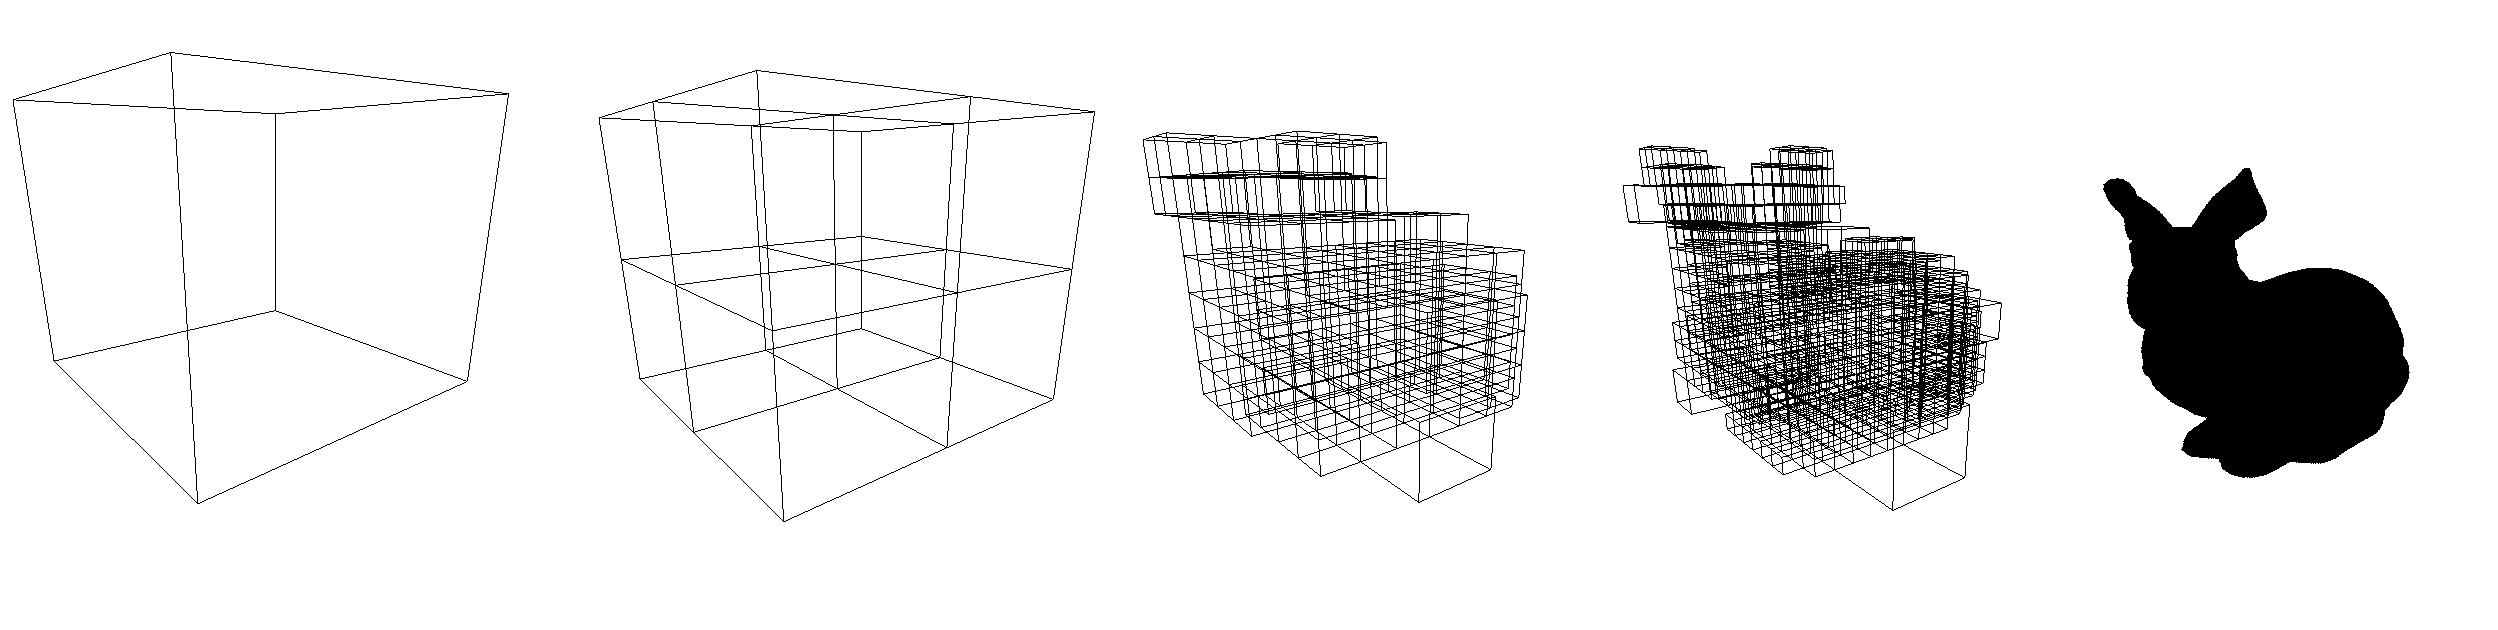
\includegraphics[width=14cm]{images/ch2/OctreeExample}
\caption{An Example of an Octree used to represent an object at differing levels of accuracy \cite{Hornung13Octomap}. Left: Original model, Middle: few node splits used to represent the model. Right: many node splits used to more accurately represent the model.}
\label{fig:octreeaccuracy}
\end{figure}


\subsubsection{Octree Description}
\label{OTDesc}

The Octree is the three dimensional extension to the two dimensional Quad-Tree (QT) technique. First we provide some information about the QT and the idea behind using planes or shading the cubic (or square in the case of the QT) nodes to improve compression and efficiency. This was the fundamental idea behind the Shade-Tree and ILQT algorithms \cite{Gonzalez07ShadeTree, Lincoln13Interpolating}. Both these techniques have been shown to improve compression in comparison to state of the art transforms and form the basis of reasoning behind the Plane-Tree. \\

The QT is a hierarchical data structure used for processing and compressing 2D data. Figure \ref{QuadtreeExample} shows an example of a QT used to represent an image. In this figure, the original image is on the left. The QT first uses a single coloured square to represent the entire image, then using some error metric it decides whether or not to, a) represent the image more accurately using more memory or b) stop decomposition and represent the image with a single colour. If option b) is chosen, the image will look like the second left picture. If option a) is chosen, the image is divided into four sub-images each with its own colour. From here the whole process begins again, with each sub-image given the same options. The final product of the QT is shown on the far right in figure \ref{QuadtreeExample} and a visualization of a QT hierarchy is shown in figure \ref{QuadTreeHierarchy}. \\


\begin{figure}[!htb]
\centering
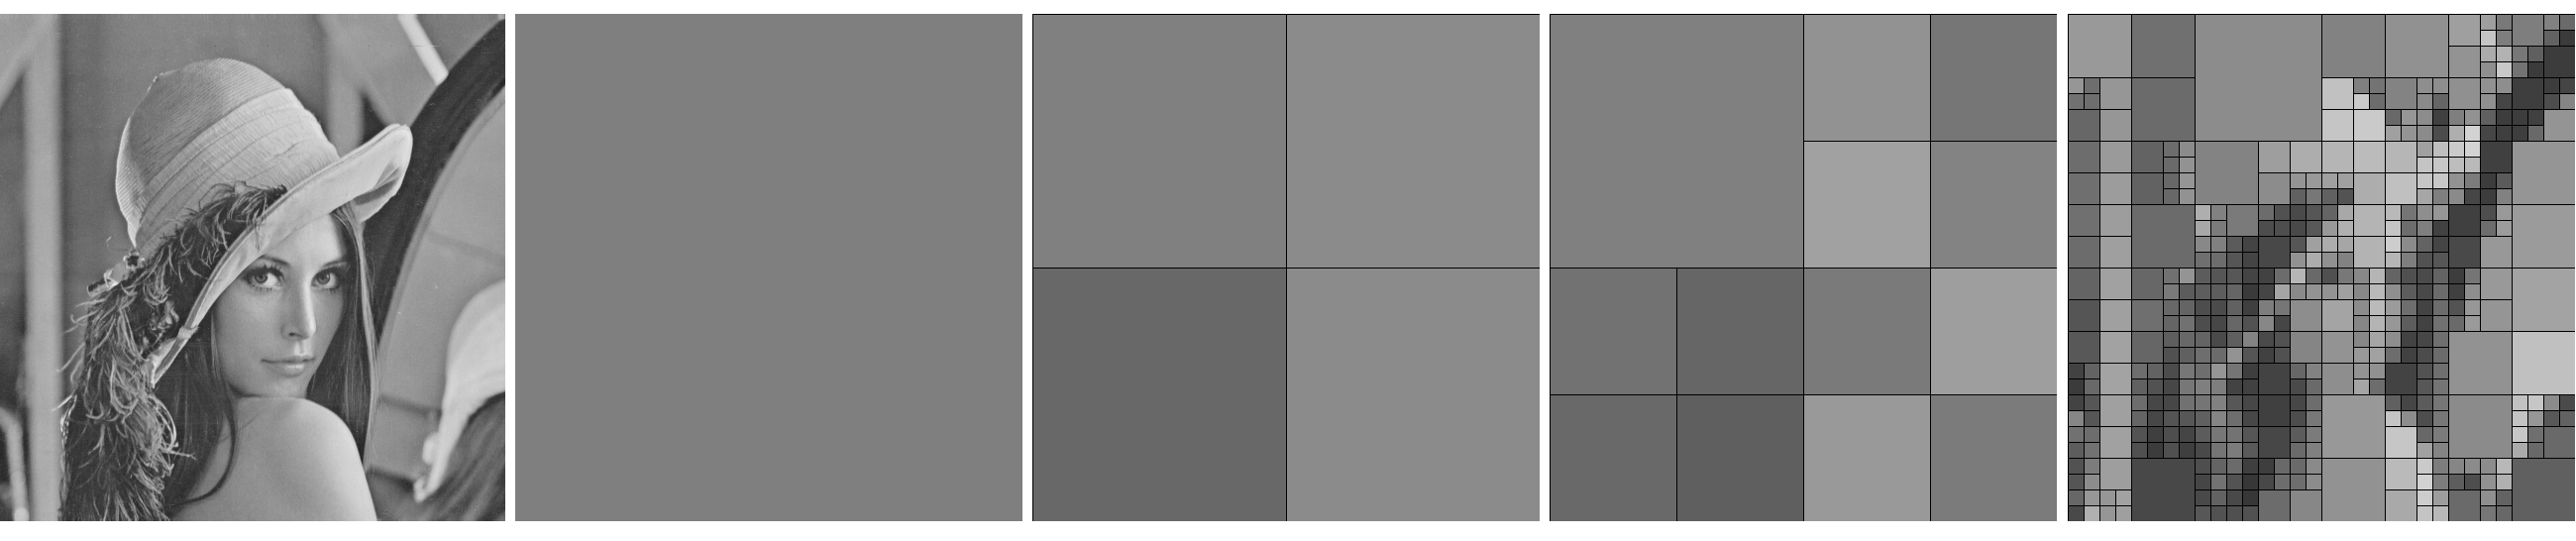
\includegraphics[width=12cm]{images/ch2/quadtreeexample}
\caption{Quadtree Image Representation, left to right: Original Image, 1st Level of Decomposition, 2nd Level of Decomposition, 3rd Level of Decomposition, QT codec Image.}
\label{QuadtreeExample}
\end{figure}


\begin{figure}[!htb]
\centering
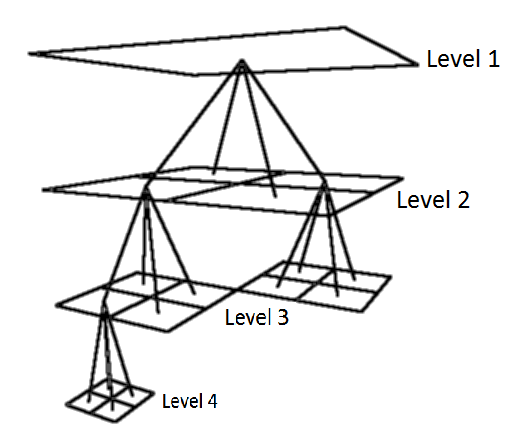
\includegraphics[width=6cm]{images/ch2/QuadTreeHierarchy}
\caption{A visualization of the QT hierarchy}
\label{QuadTreeHierarchy}
\end{figure}

The ILQT and Shade-Tree use small amounts of memory at the corners of the quadrants and interpolate to generate the underlying structure. The small data structures used for representation are much more compressed in their representation compared to the raw pixel data. For this reason, the ILQT and Shade-Tree do not need to decompose as much as other representations and allow for greater compression as proven by their ability to compete with transform based methods. \\

As mentioned, the OT works identically to the QT but in 3D. Instead of surrounding the 2D image with a square encompassing the entire frame, a cube is used to enclose the 3D space. Similarly to the QT, an error metric is used to decide whether the current representation is adequate enough or not. If the octant must be split, it is divided into eight sub-octants. Each split operation divides each coordinate ($x,y,z$) by two, giving the 8 sub-octant spaces. Figure \ref{OctreeExample} shows and example of this decomposition process. The further each cube is split, the more the OT resembles the model being compressed. In the QT and OT, nodes which have not been split are called leaf nodes and the function which decides whether a node should be split is called a leaf criterion function. \\ 

\begin{figure}[!htb]
\centering
\includegraphics[width=16cm]{images/ch2/OctreeExample}
\caption{Visualization of OT Decomposition}
\label{OctreeExample}
\end{figure}

The goal of the OT and the QT is to store the size and attributes of each node implicitly. There are two main methods of representation, a packed traversal of the tree and a linear tree. The packed traversal method stores the hierarchy using a pre-defined traversal of the tree, and typically follows one of two orderings. These are, breadth-first traversal and depth-first traversal, these orderings are shown in figure \ref{TreeTraversalExample}. The depth-first traversal starts at the root, then works it's way down, top to bottom, then left to right of the tree. In essence, it travels to a node's children before considering its neighbours. In contrast, the breadth-first traversal goes to all nodes which are at the same depth before continuing on to lower levels. \\


\begin{figure}[!htb]
\centering
\includegraphics[width=12cm]{images/ch2/TreeTraversalExample}
\caption{Tree Traversals, Left: Depth First Traversal, Right Breadth First Traversal}
\label{TreeTraversalExample}
\end{figure}

Encoding the two packed tree traversal methods requires one nibble (4 bits) for a QT node, and one byte (8 bits) for an OT node. Here, the bits represent the structure of the sub-node. For example, the QT node bit sequence, $1001_2$ means that the node has two children (corresponding to the ones), the sequence $0000_2$ means the node is a leaf node. Each bit position indexes a child node using a pre-determined ordering. An example of a possible ordering for a quadrant and an octant is shown in figure \ref{ChildOrderExample}, both breadth-first and depth-first traversals use the same index method, the difference lies only in the order which nodes are visited. 

\begin{figure}[!htb]
\centering
\includegraphics[width=12cm]{images/ch2/ChildOrderExample}
\caption{A possible child ordering for the QT (left), and the OT (right).}
\label{ChildOrderExample}
\end{figure}

The linear tree representation stores each leaf node individually. Each leaf is encoded as the pathway from the root to the leaf itself. This method was investigated in the 1980s \cite{Gargantini82Effective,Yufei88Octcodes}, but has not been used much in modern compression algorithms due to its inefficiency compared with the packed traversal method. An example of this structure is shown in figure \ref{LinearCellCodeRepresentation}, where each node: $a$, $b$, $c$, $\dots$ , $m$  is encoded as a variable length traversal path. The QT and OT are widely used in image \cite{Varma12Application} and 3D compression \cite{Schnabel06Octree}. Hanan Samet \cite{Samet88Fund1} presents an introduction to both of these structures, he also describes both tree storage methods in depth. 

\begin{figure}[!htb]
\centering
\includegraphics[width=12cm]{images/ch2/LinearCellCodeRepresentation}
\caption{A Linear Tree Code Representation Example}
\label{LinearCellCodeRepresentation}
\end{figure}



\subsection{3D ShadeTree Coding}

\label{sec:dr:coding}

The Shade-Tree compression system \ref{Gonzalez07ShadeTree} was designed for the compression of 2D image data. However, this method is easily extended to 3D Volumetric data. In this system, Octants are decomposed in the same manner as with a regular octree but the leaf node representation is different. In the Shade-Tree, the corner values in the volume are sampled for each node. Figure XXXXFFG shows an example of these corners given an Octree. The corner values are stored instead of the data within the cube. \\


The actual data representation is formed by interpolating between these 4 corner values to generate the data within the node. This representation saves space by storing 4 corner values only rather than the dense volumetric data. The method also boasts the ability for nodes to share data. For example, if two leaf nodes happen to share a corner we can simply encode the corner once using another data structure at the decompression stage at no cost to the representation. This is illustrated in figure FEFEEF. \\

This data representation may also be used to represent Signed Distance Functions, which are now commonly used in 3d reconstruction as a means of representation. In fact, such a scheme would greatly benefit the compression method of the Shade-Tree since its data is typically represented as smooth changes along a given path. 

\subsection{PlaneTree Coding}

Our method is based on octree subdivision, it begins by placing the mesh within a cube. It checks whether the the representation corresponding to this single cube is at a desired level of quality. If it is not, the cube is decomposed into 8 sub-cubes. For each sub-cube associated with the mesh, the process repeats. This process is typically controlled using an error threshold and a maximum depth value. At each level of subdivision, the error between the sub-cube (or node) representation of the space is compared to the part of the model within the cube. If the error is below the error threshold, decomposition stops. Likewise, if the level of subdivision is greater or equal to the maximum depth value, decomposition also stops. \\

In the typical octree node representation, the raw cube is used to represent the space. Unless this cube is small (deep within the tree) the error is typically high. Trees which are very deep require more storage space. Our method stores arbitrary first order planes within nodes at 20 bits per leaf. This small bit cost per leaf node greatly improves compression performance compared to the octree and makes it competitive with state of the art methods. \\

 
In the following sections, we present the details of the Plane-Tree in terms of subdivision, leaf node plane computation and representation as well as compression and decompression.


\subsection{Octree Subdivision}

Prior to compression, the input 3D model is normalized into a $512^3$ space. Starting with the cube which represents this space, we compute our 3D plane representation. Then the mean squared error between the sampled points of the plane and the sampled points of the model (which lie within the cube) is computed. If this value is below a given threshold, or the maximum level of subdivision is reached, decomposition stops. Alternatively if both of these predicates are not met, the cube is divided into 8 sub-cubes. Each sub-cube is then tested to see whether part of the mesh lies within it. If so, the process it repeated for that cube, otherwise no action is taken. \\

Each cube/sub-cube is referred to as a node. Each node which has no children is referred to as a leaf node. During compression/decompression, our plane based representation is only stored at leaf nodes, with non-leaf nodes serving only as paths giving the location of leaf nodes. Below, the computation and representation of our novel leaf node representation is discussed. \\

\subsection{Leaf Node Computation and Representation}
\label{NRep}
Our novel leaf node representation better represents the mesh which intersects it compared to the octree, it does so by using a first order plane. This representation requires only 20 bits, allowing us to achieve higher quality models whilst saving on bits which would otherwise be used to form a deeper, and thus more costly octree representation. It also gives our method an advantage at low bitrates. \\

In order to generate a plane for a given leaf node, we first sample the mesh within the node space. Using these points, the x, y and z axis variances are measured. These indicate how much variation lies across each axis within the node. We then find the plane using least squares, solving for the axis with the lowest variance. Once we have coefficients describing the plane, we use a single point on the plane, and the plane normal to describe it. \\

Using a point on the plane and a plane normal, we can find a set of triangles which represent the plane within the node. We first find all points in which the cube's edges intersect with the computed plane. Using the average point as the origin, and the plane's normal as the y-axis, we order the points based on their x/z angle. This gives us an ordered set of points which corresponds to a polygon defining the plane within the node. This polygon is then triangulated forming the final representation. This process is used at both the compression and decompression stages. \\

The triangles representing the plane within the node are then sampled along with the parts of the mesh lying within the node. The mean squared error (mse) is then taken between these samples for comparison with the error threshold value. Within the summation for the mse we use the closest point within the second point set, this is shown in equation \ref{eqn:MSE_1}.

\begin{equation}
 \label{eqn:MSE_1}
MSE(pts_1, pts_2) = \frac{1}{N}\sum_{i=0}^{N} (pts_{1_i} - closest(pts_{1_i}, pts_2))^2
\end{equation}

Using this equation and the sampled points from the plane triangles $p$, and the sampled points from the mesh $m$ (which lie within the cube), we take the average of both mean squared errors as a measurement of total error, $error = \frac{1}{2}MSE(p,m) + \frac{1}{2}MSE(m,p)$. This is the value which is compared with the error threshold to decide whether decomposition should stop or not. \\

In order to compress the data for our leaf node representation, we store the the plane using its normal vector and a single point lying on the plane. We store the normal vector using 12 bits (4 bits per coordinate). The point which lies on the plane is represented using two pieces of information, an edge number and a distance variable. First it must be mentioned that for a given plane which intersects a cube, a minimum of 3 of the cube's edges pass through the plane. We therefore record one of these edges (the edge number) and the distance from on of its end points (the distance variable). Each edge has a predefined number which identifies it, all edges also have a predefined start and end point. \\

Each cube has 12 edges in total, so 4 bits are used for the edge number, another 4 are used for the distance variable. Adding these to the normal vector totals to 20 bits per leaf node representation.  \\


\subsection{Compression and Decompression}

In order to compress our data structure we iterate through the tree in depth first order. If we encounter a non-leaf node, we first store a single bit of $1_2$. Then the configuration of the sub-nodes (since not every sub-node intersects the object) is stored as a single byte. Each bit is labelled $1_2$ if a particular sub-node exists and $0_2$ if it does not. This is possible since we order our sub-nodes in a predefined order. If a leaf node is encountered, we store a $0_2$, then record our 20 bit leaf node representation in three other files. One for the normal data, the distance variables and edge numbers totalling 4 files (tree, normals, distances and edge numbers). After the entire structure is stored we employ entropy encoding on each of these files. \\

In order to decompress our structure, we read the first bit of the output file. This checks if the current node is a leaf or not. If it is, we read out a 20 bit plane representation (from the three separate files) and generate a list of triangles representing where the plane intersects the node (explained in section \ref{NRep}). These triangles are then added to a final database which represents the decoded model. If we reach a non-leaf node, we read out the 8 bit sub-node configuration and repeat the process for each existing sub-nodes in the predefined order. \\  

 % Methodology
\begin{savequote}[8cm]
  ``I just wondered how things were put together.''
  \qauthor{Claude Shannon}
\end{savequote}
\makeatletter
\chapter{Experiments}

\section{Experiments}

\section{Test Data}

Test Data was generated based on the testing requirements for this research. In order to robustly test the different pose-estimation procedures / 3D-registration methods we generated data from a variety of scenes. These scenes include both in-door and out-door scenes, scenes with large amounts of texture and scenes with little to no texture. We also captured scenes which may cause confusion for algorithms which rely on texture information. This data typically has many items which look similar locally but are actually different objects within the scene globally. \\

Moreover, our test-data also measure's each algorithm's ability to register different camera movements by localizing them to different scenes. Different camera motions captured include: camera translation and zooming as well as different axes of rotation. \\

Some frames from the original test-set are shown in appendix \ref{AppendixA}. The first scene: the Apartment Texture Rotate scene was taken by rotating the camera around the y-axis across an apartment. This scene contains plenty of textural information. The Apartment Texture X Axis scene is similar in terms of texture but contains both x and y axis rotation. This tests the Volume Phase Registration algorithm's ability to handle multiple axes of rotation. \\

The boxes scene was captured under arbitrary-rotation, translation and zoom-in/out camera motions. It contains some useful information on the boxes themselves, however the texture on the carpet is of little to no use for most feature based registration methods. The Desk Texture Translation scene contains a desk with a desktop computer and several items on it. The In-door space with texture-confusion contains a set of chairs and picture frames which look similar to eachother locally but may cause confusion for registration techniques which rely on local features.  \\

The kitchen scene was captured with both translation and zoom camera movements. The scene contains very little texture and the color is predominantly white. The Office textured blind-spot rotation scene is a textured office scene where the camera is rotated about the y-axis. The scene is focused on a large divider which seperates two desks. The divider may confuse registration methods which rely too heavily on minimization by aligning the large divider in priority rather than taking into acount the smaller details of the scene. \\

The Office scenes contain a decent amount of usable texture and different sets were created by translating, rotating about the y-axis and rotating about the x-axis. Other office scenes, where the camera has objects in both the foreground and the background and where the camera is lifted and rotated whilst focusing on an office desk/chair. \\

Some out-door scenes were also captured around the university. Scenes are captured with both rotation and translation camera movements. These scenes are also labelled as being susceptable to texture confusion.

\section{Analysis Tools}

In order to test different registration methods. Algorithms were written in C/C++ using both Visual Studio (2012 and 2015) on a Windows (7 \& 10) machine and code-blocks 16 on an Ubuntu machine. All source code is made available online at: https://github.com/lukes611/phdThesis. In order to measure registration algorithms we use the error metrics described in the ERROR METRICS SECTION section.  

\section{Algorithms}

Different 3D-registration algorithms were implemented to test the Fourier Volume Registration (FVR) method. We compared with Feature Matching methods because these methods are still dominant and very successful in image processing and computer vision. In this research we aimed to show that FVR was competitive with these feature matching methods whilst beating them in certain contexts (such as little textuere or scenes where texture confusion may occur). \\ 

We test with both 2D feature matching, where the features are found and matched between a pair of 2D-images, then RANSAC is used with the corresponding matches and true 3D point to compute pose. The pose is then used to reconstruct the scene. We found that SURF performed best out of the other feature matching methods, so we use SURF in our 2D feature matching algorithm. The 2D feature matching method is limited as it cannot register frames which have too few features or frames which contain texture confusion. It is also not able to handle wider base-lines. \\

We also test 3D-feature matching using an implementation of SIFT in 3D. This algorithm was tested and written in C/C++ and is also susceptable to failed registration in scenes with too few features and texture confusion but it shouble be more able to handle wider base-lines than the 2D counterpart as it works in 3D. //

Another algorithm we test against is ICP or Iterative Closest Point. This method has become very popular in 3D reconstruction and works well on most scene types. One disadvantage is that this method may get stuck in a minima and fail to register, this can occur especially when registering wider baselines. \\

The other method we test with is PCA or Principal Components Analysis is actually used to find the mean and principal components of a multi-dimensional data-set. This is useful for registration purposes as it works on wide-baselines, is very fast and provides additional information about a scene. The downside is that is is very susceptable to noisey or mis-aligned data. Our FVR method actually makes use of information from PCA so it is good to compare the two to find out what improvements if any are made by FVR. \\

The final algorithm tested is the proposed FVR algorithm, which uses both PCA and Fourier Phase Correlation to find the registration transformation between two 3D data-sets. This algorithm was proposed to handle general transformations about any rotation axis, translation axis as well as handle scaling. It was also designed to be able to handle noisey data, data with texture-confusion and data with little to no texture making it a viable option in the 3D registration and pose estimation research areas.


\section{Qualitative Experiments}

Our Qualitative experiments were performed by using different algorithms to generate 3D reconstructed scenes. 

\section{Quantitative Experiments}

\subsection{Camera Movement Experiments}

\subsection{Pose Estimation Experiments}

\subsection{Noise Experiments}




\begin{figure*}[t] 
        \centering
        \begin{subfigure}[b]{2.0in}
                \includegraphics[width=2.0in]{images/ch2/unit21}
                \caption{Apartment}
                \label{fig:RECON_UNIT}
        \end{subfigure}%
        \begin{subfigure}[b]{2.0in}
                \includegraphics[width=2.0in]{images/ch2/officeA}
                \caption{Office}
                \label{fig:RECON_OFFICE}
        \end{subfigure}%
        \begin{subfigure}[b]{2.0in}
                \includegraphics[width=2.0in]{images/ch2/outdoorA}
                \caption{Garden}
                \label{fig:RECON_GARDEN}
        \end{subfigure}
       \caption{Reconstructed Scenes.}
       \label{fig:RECONSTRUCTIONS}
\end{figure*}


\subsection{Codec Evaluation \& Comparison Techniques}

Codec evaluation involves comparing storage requirements between the original model and codec output. In the case of lossy codecs, a quantitative quality metric is also required. Compression metrics are easy to compute, quality metrics are more involved and there have been many proposed techniques. Quality metrics compare the distortion created by the codec relative to the original model. Two measurements are usually performed, the distance from the compressed model to the original and the distance from the original to the compressed model. Quality metrics are split into empirical and perceptual based metrics. Empirical metrics measure geometric error and perceptual metrics estimate human perception. Perception based metrics are a part of psychophysics research. For a more in-depth survey of these methods, see work by Bubill \textit{et al.} \cite{Bulbul11Assessing}.

\subsubsection{Compression Metrics}

In the context of 3D model compression, the file size of both, the compressed model and the original are compared. Alternatively, the file size of the compressed model from one codec can be compared to the file size of the same model compressed using another codec. The compression ratio ($CR$), defined as the original file size divided by the compressed file size, is a measure of compression performance. Another metric used is called the bit rate, different bit rates are used depending on the representation being compressed. The mesh representation uses bits per vertex (bpv) and bits per triangle (bpt), the volumetric representation uses bits per voxel and the point cloud representation uses bits per point.

\subsubsection{Empirical Error Metrics}

The following metrics are used to assess the error between two data samples. For two points, $p$ \& $q$, in $\Re^3$ space, the basic euclidean distance metric,
$$
ED(q,p) = \sqrt{(q_x - p_x)^2 + (q_y - p_y)^2 + (q_z - p_z)^2}
$$,
the absolute error,
$$
AE(q,p) = \|q_x - p_x\| + \|q_y - p_y\| + \|q_z - p_z\|
$$
and the squared error $SE$, 
$$
SE(q,p) = (q_x - p_x)^2 + (q_y - p_y)^2 + (q_z - p_z)^2
$$
are often used as a basis for other metrics. 3D models can be sampled into a set of points in $\Re^3$. Using these samples, the following metrics can be used: sum of distances ($SOD$), sum of absolute differences ($SAD$), sum of squared errors ($SSE$), mean square error ($MSE$) and root mean square error ($RMS$). Since the two models may be sampled differently, the minimum error from one sample to the others is used. These metrics are defined below using two point sets, $A$ \& $B$ where the length of these sets is $M$ and $N$ respectively.
$$
SOD(A,B) = \sum_{k=0}^{M} \min_{b \in B}(ED(A_k,b))
$$

$$
SAD(A,B) = \sum_{k=0}^{M} \min_{b \in B}(AE(A_k,b))
$$

$$
SSE(A,B) = \sum_{k=0}^{M} \min_{b \in B}(SE(A_k,b))
$$

$$
MSE(A,B) = \frac{1}{M}SSE(A,B)
$$

$$
RMS(A,B) = \sqrt{MSE(A,B)}
$$

For each of these metrics, $METRIC(A,B) \neq METRIC(B,A)$. Therefore, these methods are often averaged (below). This is termed the average metric (AM), as opposed to the minimum metric (MM) which is the smallest value of the two.

$$
AvgError = \frac{Metric(A,B)+Metric(B,A)}{2}
$$

Another metric, the Hausdorff distance ($HD$) is a measure of overall shape similarity. It is defined as the largest value of the maximum distances between objects from $A$ to $B$ and from $B$ to $A$. For example, for two objects $A$ \& $B$, the Hausforff distance $HD$, from $A$ to $B$, is defined as,
$$
HD(A,B) = \max(D(A,B),D(B,A))
$$
where $D(A,B)$ is defined as,
$$
D(A,B) = \{a \in A \| \max(dist(a,B)\}
$$
and $dist(a,B)$ is defined below.
$$
dist(a,B) = \{b \in B \left| \min(\|a-b\|)\right.\}
$$

\subsubsection{Human Perception Based Metrics}

Lavoue \textit{et al.} \cite{Lavoue06Perceptually} devised a metric based on structural distortion, this method correlates well with human perception. It is based on the SSIM method of Wang \textit{et al.} \cite{Wang04Image}, which is a popular image metric. Lavoue \textit{et al.} call their method the, Mesh Structural Distortion Measure (MSDM). An updated version of this metric was also developed \cite{Lavoue11Multiscale}.

\paragraph{Laplacian Metric}

Karni \& Gotsman \cite{Karni00Spectral} developed their own on-line metric for use during their spectral based codec. It is based on the laplacian and measures the difference between two objects in terms of their smoothness. 

\paragraph{Elastic Deformation Based Metric}

Bian \textit{et al.} \cite{Bian09Evaluation} developed a novel metric, useful for both on and off-line model comparison. The algorithm is based on the theory of strain fields. A strain field is a metric derived from elasticity, it is used to describe the deformation of some object which has elastic properties. Using this concept, both models are treated as having elastic properties in order to perform quality assessment.

\paragraph{Saliency Based Metrics}

Howlett \textit{et al.} \cite{Howlett04Experimental} and Lee \textit{et al.} \cite{Lee05Mesh} both presented work aimed at determining salient features in 3D models. They incorporated these findings in their own metrics. Howlett \textit{et al.} used a human gaze detection device to study the psychophysical effects of viewing 3D objects. Both of these metrics are based on preserving the sections of the object in which any distortion would be visibly noticeable to humans.

\paragraph{The Depth Difference Metric}

Krivokuca \textit{et al.} \cite{Krivokuca12New} developed a perceptual based metric for the off-line quality assessment of 3D models. This method is independent of model representation and is based on generating multiple depth maps from different orthographic perspectives. It improves upon both the Hausdorff distance and RMS error and is good at detecting both small and large geometric errors. Krivokuca \textit{et al.} call their method, the Depth Difference (DD). It works by comparing orthographic depth maps from both the original and compressed models. First a difference depth image is calculated ($DDI$) from orthographic depth maps of the original object ($DIO$) and of the compressed object ($DIC$). The $DDI$ is calculated using element-wise matrix subtraction,

$$
DDI = DIO - DIC
$$

Then the average depth distance value ($ADD$) is calculated from the $DDI$ matrix, this equation is presented below.

$$
ADD = \frac{1}{MN} \sum_{y=0}^{M} \sum_{x=0}^{N} DDI_{y,x}
$$

This $ADD$ value is then summed up and averaged over different orthographic views, this average is the Depth Difference.

 % Experiments &
\section{Results}

%in methodology section?
\section{Test Data}

\section{Analysis Tools}

\section{Qualitative Experiments}

\section{Quantitative Experiments}

\subsection{Pose Estimation Experiments}

\begin{figure*}[t!] 
        \centering
        \begin{subfigure}[b]{6.0in}
                \includegraphics[width=6.0in]{images/results/Apartment_Texture_Rotate}
                \caption{original}
                \label{fig:PEE1}
        \end{subfigure}
       \caption{Registration improvements for Apartment Texture Rotate for different methods.}\label{fig:PEE1Fig}
\end{figure*}

\begin{figure*}[t!] 
        \centering
        \begin{subfigure}[b]{6.0in}
                \includegraphics[width=6.0in]{images/results/Apartment_Texture_Rotate_XAxis}
                \caption{original}
                \label{fig:PEE2}
        \end{subfigure}
       \caption{Registration improvements for Apartment Texture X-Axis Rotate for different methods.}\label{fig:PEE2Fig}
\end{figure*}


\begin{figure*}[t!] 
        \centering
        \begin{subfigure}[b]{6.0in}
                \includegraphics[width=6.0in]{images/results/Boxes_Texture_Rotate}
                \caption{original}
                \label{fig:PEE3}
        \end{subfigure}
       \caption{Registration improvements for Boxes Texture Rotate for different methods.}\label{fig:PEE3Fig}
\end{figure*}

\subsection{3D Registration Experiments}

\subsection{Noise Robustness Tests}

hi


\section{Conclusion}
 % Results
\begin{savequote}[8cm]
  ``Learn from yesterday, live for today, hope for tomorrow. The important thing is not to stop questioning.''
  \qauthor{Albert Einstein}
\end{savequote}
\makeatletter
\chapter{Conclusion}

\section{Research Aims Revisited}

The primary aim of this research was to improve the storage, quantitative quality and perceptual quality of 3D models. Hierarchical methods were investigated and this led to a new image codec, ILQT \cite{Lincoln13Interpolating} as well as the proposed scheme, the Shade-Octree. The research question was, ``Do hierarchical techniques bring state of the art compression performance to 3D data?'' Results from chapter 4 show that the SOT outperforms the OT compression scheme as well as several state of the art methods in terms of rate-distortion and perceptual quality. The primary aim of this research has been accomplished because the SOT produces models which have improved storage efficiency, whilst improving quantitative quality and perceptual quality compared with other compression schemes. The proposed research question can also be answered. The SOT, a hierarchical codec, does achieve state of the art performance in the field of 3D data compression.

\section{Future Work}

There is still much work to be done in the area of hierarchical 3D data compression. One possible project could be to improve the SOT. Currently the SOT can produce holes in the output mesh, an investigation of this may lead to improved results. Other projects could investigate the extension of the PJQ, wedglet, BSP-tree and QB tree to 3D model compression.
 % Conclusion
\appendix
none
\makeatletter
\chapter{Appendix A}
\label{AppendixA}

\section{Test Data}

%keep
\begin{figure*}[t]
\centering
\begin{subfigure}[b]{1.5in}
\includegraphics[width=1.5in]{{images/experiments/test_data/Apartment.Texture.rotate.0}.png}
\caption{Frame 1}
\end{subfigure}%
\begin{subfigure}[b]{1.5in}
\includegraphics[width=1.5in]{{images/experiments/test_data/Apartment.Texture.rotate.1}.png}
\caption{Frame 10}
\end{subfigure}%
\begin{subfigure}[b]{1.5in}
\includegraphics[width=1.5in]{{images/experiments/test_data/Apartment.Texture.rotate.2}.png}
\caption{Frame 15}
\end{subfigure}%
\begin{subfigure}[b]{1.5in}
\includegraphics[width=1.5in]{{images/experiments/test_data/Apartment.Texture.rotate.3}.png}
\caption{Frame 20}
\end{subfigure}%
\caption{Four Sample Frames from the Apartment Texture Rotate Data Set}
\label{fig:Apartment_Texture_rotate}
\end{figure*}


%keep
\begin{figure*}[t]
\centering
\begin{subfigure}[b]{1.5in}
\includegraphics[width=1.5in]{{images/experiments/test_data/Apartment.Texture.rotateXAxis.0}.png}
\caption{Frame 1}
\end{subfigure}%
\begin{subfigure}[b]{1.5in}
\includegraphics[width=1.5in]{{images/experiments/test_data/Apartment.Texture.rotateXAxis.1}.png}
\caption{Frame 10}
\end{subfigure}%
\begin{subfigure}[b]{1.5in}
\includegraphics[width=1.5in]{{images/experiments/test_data/Apartment.Texture.rotateXAxis.2}.png}
\caption{Frame 15}
\end{subfigure}%
\begin{subfigure}[b]{1.5in}
\includegraphics[width=1.5in]{{images/experiments/test_data/Apartment.Texture.rotateXAxis.3}.png}
\caption{Frame 20}
\end{subfigure}%
\caption{Four Sample Frames from the Apartment Texture X-Axis Rotation Data Set.}
\label{fig:Apartment_Texture_rotateXAxis}
\end{figure*}


%keep
\begin{figure*}[t]
\centering
\begin{subfigure}[b]{1.5in}
\includegraphics[width=1.5in]{{images/experiments/test_data/Desk.Texture.Translation.0}.png}
\caption{Frame 1}
\end{subfigure}%
\begin{subfigure}[b]{1.5in}
\includegraphics[width=1.5in]{{images/experiments/test_data/Desk.Texture.Translation.1}.png}
\caption{Frame 10}
\end{subfigure}%
\begin{subfigure}[b]{1.5in}
\includegraphics[width=1.5in]{{images/experiments/test_data/Desk.Texture.Translation.2}.png}
\caption{Frame 15}
\end{subfigure}%
\begin{subfigure}[b]{1.5in}
\includegraphics[width=1.5in]{{images/experiments/test_data/Desk.Texture.Translation.3}.png}
\caption{Frame 20}
\end{subfigure}%
\caption{Four Sample Frames from the Desk Texture Translation Data Set.}
\label{fig:Desk_Texture_Translation}
\end{figure*}


%keep
\begin{figure*}[t]
\centering
\begin{subfigure}[b]{1.5in}
\includegraphics[width=1.5in]{{images/experiments/test_data/Office.Texture.blindSpotRotation.0}.png}
\caption{Frame 1}
\end{subfigure}%
\begin{subfigure}[b]{1.5in}
\includegraphics[width=1.5in]{{images/experiments/test_data/Office.Texture.blindSpotRotation.1}.png}
\caption{Frame 10}
\end{subfigure}%
\begin{subfigure}[b]{1.5in}
\includegraphics[width=1.5in]{{images/experiments/test_data/Office.Texture.blindSpotRotation.2}.png}
\caption{Frame 15}
\end{subfigure}%
\begin{subfigure}[b]{1.5in}
\includegraphics[width=1.5in]{{images/experiments/test_data/Office.Texture.blindSpotRotation.3}.png}
\caption{Frame 20}
\end{subfigure}%
\caption{Four Sample Frames from the Office Texture.blind-spot Rotation Data Set.}
\label{fig:Office_Texture_blindSpotRotation}
\end{figure*}


%keep
\begin{figure*}[t]
\centering
\begin{subfigure}[b]{1.5in}
\includegraphics[width=1.5in]{{images/experiments/test_data/Office.TexturedItems.Translation.0}.png}
\caption{Frame 1}
\end{subfigure}%
\begin{subfigure}[b]{1.5in}
\includegraphics[width=1.5in]{{images/experiments/test_data/Office.TexturedItems.Translation.1}.png}
\caption{Frame 10}
\end{subfigure}%
\begin{subfigure}[b]{1.5in}
\includegraphics[width=1.5in]{{images/experiments/test_data/Office.TexturedItems.Translation.2}.png}
\caption{Frame 15}
\end{subfigure}%
\begin{subfigure}[b]{1.5in}
\includegraphics[width=1.5in]{{images/experiments/test_data/Office.TexturedItems.Translation.3}.png}
\caption{Frame 20}
\end{subfigure}%
\caption{Four Sample Frames from the Office Textured Items Translation Data Set.}
\label{fig:Office_TexturedItems_Translation}
\end{figure*}


%keep
\begin{figure*}[t]
\centering
\begin{subfigure}[b]{1.5in}
\includegraphics[width=1.5in]{{images/experiments/test_data/Office.Texture.rotation.0}.png}
\caption{Frame 1}
\end{subfigure}%
\begin{subfigure}[b]{1.5in}
\includegraphics[width=1.5in]{{images/experiments/test_data/Office.Texture.rotation.1}.png}
\caption{Frame 10}
\end{subfigure}%
\begin{subfigure}[b]{1.5in}
\includegraphics[width=1.5in]{{images/experiments/test_data/Office.Texture.rotation.2}.png}
\caption{Frame 15}
\end{subfigure}%
\begin{subfigure}[b]{1.5in}
\includegraphics[width=1.5in]{{images/experiments/test_data/Office.Texture.rotation.3}.png}
\caption{Frame 20}
\end{subfigure}%
\caption{Four Sample Frames from the Office Texture Rotation Data Set.}
\label{fig:Office_Texture_rotation}
\end{figure*}



\chapter{Appendix B}
\label{RawQuantitative1}

\section{Registration Errors}

\chapter{Appendix C}
\label{RawQuantitative2}

\section{Noise Results} % Appendix A
\backmatter
\openup -0.5em
%\bibliographystyle{plain}
\bibliographystyle{IEEEtran}
\bibliography{bibliographies/slam,bibliographies/compress}
\end{document}